\begin{multicols}{2}
	
	\section{Introduction}
	
	The history of science is not free from injustices. Henri Poincaré,
	from whom Einstein borrowed the tools to create special relativity,
	has fallen into oblivion, while Einstein received the spotlight 
	from everyone.
	
	The same goes for Louis de Broglie. Many criticized him for 
	clinging to a realistic vision of physics, seeking a
	meaning behind the pure mathematical abstractions of quantum 
	mechanics. Unfortunately, he only lacked the language to 
	prove his brilliant visions. By a second irony of history, 
	this language was nevertheless born contemporaneously with de Broglie: it is 
	algebraic geometry. May the success of quantum plenodynamics 
	refocus the spotlight on this man whose trace history has almost 
	erased, except for his famous equivalence formula 
	between momentum and frequency.
	\medskip
	
	Physical theories are never born from nothing. According to Henri 
	Poincaré \cite{poincare:1902:sh}, the physicist attempts 
	to extrapolate a theory from experimental facts. These are two 
	traces, two points, from which the physicist extrapolates a law. 
	In reality, there is an infinite number of ways to extrapolate a law, for there is an infinite number of ways to connect two experimental points. Physics --~at least until quantum mechanics~-- 
	has always postulated continuity between the two points, as well as the 
	principle of least action of Maupertuis, which is the natural way 
	to minimize energy by taking the "shortest path". Another 
	way of seeing this principle is the application of the principle of 
	Occam's razor: among all possible theories, the best 
	is the simplest, which is yet another way of saying that 
	simplicity goes hand in hand with beauty. This is one of two pivots upon 
	which the creation of quantum plenodynamics was articulated. The 
	second pivot is that of anchoring in reality, dear to Albert 
	Einstein\footnote{"I cannot believe that God plays dice. [$\dots$] If physics does not represent reality, it is only a diversion for mathematicians." \cite{EinsteinBorn2005}}. \cite{einstein1949autobiographical} And to Louis de Broglie. \cite{debroglie1976physique}
	
	Physicists have therefore developed remarkable theories from 
	their experimental points. They then tried to link the 
	theories assuming they were correct, since they 
	worked. A theory of everything therefore had to start from one of these 
	theories and absorb the others. But not for a moment did they think 
	that these theories were only very good approximations and that 
	from an approximation, it was not possible to bring forth 
	a finer and more encompassing model.
	
	It is possible also that another factor played a role. Since the 
	"approximate" theories were very complicated, then the theory 
	of the whole had to be even more complicated. It turns out that 
	fundamentally, the theory of quantum plenodynamics started 
	from the opposite postulate. The model that structures the universe, life or 
	science, must be a simple model, accessible to all, at least in 
	its general explanation. Physical meaning must be able to be explained and 
	understood. After all, is physics not \textit{stricto sensu} 
	the application of two elementary principles, causality and 
	action-reaction which, they too, are perfectly understandable to 
	all? Simplicity, beauty and reality. Here are the three pillars of 
	quantum plenodynamics!
	
	This is the reason why this present article will be presented from 
	two angles. The first is ontological and practical, almost purely 
	mechanical. We will see where the theory comes from, what choices 
	presided over its birth and development. The second is more 
	mathematical. We will see how to apply a topology and especially a 
	metrology to the model, which will obviously --~and without surprise~-- be a 
	Clifford algebra, reinforcing the model while allowing it 
	to add a structural finesse that a simple ontological analysis 
	does not allow, such as the shapes that the elementary particles 
	of the standard model can take.
	
	However, plenodynamics does not come out of a hat and 
	it originates from experimental results provided by 
	quantum mechanics. It could undoubtedly have been based on 
	quantities extracted from gravity, but by a sort of scale 
	reflex, which is not without irony for a fractal theory, 
	the idea first crystallized around the smallest 
	structures of physics. It is not the least of paradoxes to 
	build a Fundamental Physics of the Universe from 
	results of approximate physics. In reality, the loop is 
	closed, in the sense that quantum plenodynamics is indeed based on 
	experimental values --~the famous two starting points~--, but 
	this time without omitting any.
	
	If the first part is intended to be more literary, it does not 
	address a novice audience in physics. It postulates a 
	general knowledge of all current physics. This is not 
	innocent: quantum plenodynamics contains the seeds of all 
	physics!
%	\vfill\pagebreak
	\clearpage
	
	\section{On the existence of a structure of the vacuum}
	
	\vspace*{-0.8cm}
	\begin{center}
		\begin{longtblr}[
			%theme=widecaption 
			caption={\footnotesize{\textbf{Energy of elementary particles}}},
			%label = {tblr:4-2},
			]{
				colspec={Q[c, co=1] Q[c, co=1] },
				rowspec={Q[m]},
				row{odd}={bg=blue!10!white},
				row{1}={c,mode=text,fg=white,bg=pkcolor, cmd=\textbf}, %cmd=\textbf, blue!80!orange
				rowsep=2pt, colsep=3pt,
				vline{2-Y} = {1}{0.3pt,gray!50},
				vline{2-Y} = {2-Z}{0.3pt,gray!30},
				hline{Z} = {0.1pt,blue},
				% nombre de col début et fin qui apparaissent à chaque page
				% 1 pour le titre par exemple
				rowhead = 1, %rowfoot = 1, 
			}
			Particles               &   Mass                     \\
			Photon                   &    0                        \\
			Gluon                    &    0                        \\
			Electron neutrino     &    < 0.8 $eV/c^2$           \\
			Muon neutrino        &    < 0.17 $MeV/c^2$        \\
			Electron                 &    0.511  $MeV/c^2$        \\
			Quark up (u)             &    $\approx$ 2.2 $MeV/c^2$ \\
			Quark down (d)           &    $\approx$ 4.7 $MeV/c^2$ \\
			Tau neutrino          &    < 18.2 $MeV/c^2$        \\
			Muon                     &    105.7 $MeV/c^2$          \\
			Quark strange (s)        &    $\approx$ 95 $MeV/c^2$  \\
			Quark charm (c)          &    $\approx$ 1.28 $GeV/c^2$\\
			Tau                      &    1.77 $GeV/c^2$           \\
			Quark bottom (b)         &    $\approx$ 4.18 $GeV/c^2$\\
			Boson W                  &    80.4 $GeV/c^2$           \\
			Boson Z                  &    91.2 $GeV/c^2$           \\
			Higgs boson            &    125.1 $GeV/c^2$          \\
			Quark top (t)            &    $\approx$ 173 $GeV/c^2$ \\
		\end{longtblr}
	\end{center}
	\vspace*{-0.2cm}
	\begin{center}
		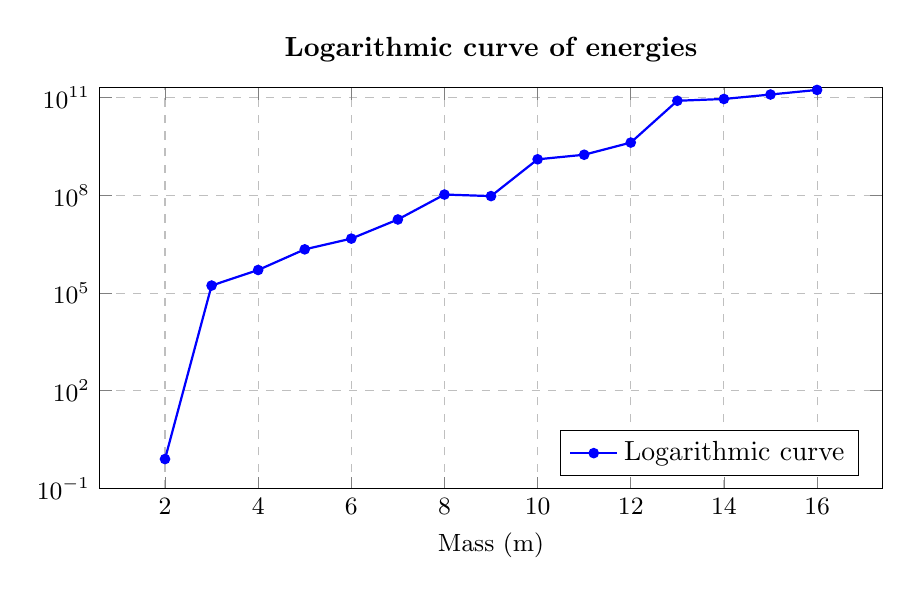
\begin{tikzpicture}
			\begin{axis}[
				width=0.95\columnwidth,          % <-- largeur exacte de la page
				height=0.55\columnwidth,     % hauteur proportionnelle (tu peux ajuster)
				%width=14cm,
				%height=9cm,
				xlabel={Mass (m)},
				ylabel={},
				title={Logarithmic curve of energies},
				xmajorgrids=true,
				ymajorgrids=true,
				grid style=dashed,
				ymode=log,                  % <--- échelle logarithmique sur l'axe y
				log basis y=10,
				ymin=0.1,                   % pour éviter le log(0)
				ymax=2e11,
				xlabel style={font=\small},
				ylabel style={font=\small},
				title style={font=\bfseries},
				tick label style={font=\small},
				legend pos=south east,
				]
				
				% Données (x = indice, y = valeur)
				\addplot[
				color=blue,
				thick,
				mark=*, 
				mark size=1.5pt,
				] coordinates {
					(0,0)
					(1,0)
					(2,0.8)
					(3,1.70E5)
					(4,5.11E5)
					(5,2.20E6)
					(6,4.70E6)
					(7,1.82E7)
					(8,1.06E8)
					(9,9.50E7)
					(10,1.28E9)
					(11,1.77E9)
					(12,4.18E9)
					(13,8.04E10)
					(14,9.12E10)
					(15,1.25E11)
					(16,1.73E11)
				};
				
				\legend{Logarithmic curve}
				
			\end{axis}
		\end{tikzpicture}
	\end{center}
	\vspace*{-0.5cm}
	
	The masses of the elementary particles of the standard model of 
	physics clearly show a log-periodic dispersion. There 
	exists therefore a generating element that follows a normal law allowing 
	for the reconstitution of elementary particles. This element depends \textit{a 
		minima} on a distance and a time (dual-scale structure) and follows a 
	fractal law.
	
	It is reasonable to think that this element is the structure of the vacuum. 
	
	\begin{mybox}[breakable,colback=blue!10, colbacktitle=pkcolor]{Postulate 1}
		The vacuum is not empty, but is made from a single element.
	\end{mybox}
	\medskip
	
	In a deliberate manner, quantum plenodynamics starts \textit{a contrario} from 
	received ideas. The aether exists and we are going to build it. Einstein, who 
	demonstrated that the luminiferous aether, the fluid of the \textsc{xix}\textsuperscript{th} century, did not exist, 
	was not \textit{stricto sensu} opposed to it. At the University of 
	Leiden, on May 5, 1920, he stated \cite{einstein1920ether}: "In 
	summary, we can say that according to the general theory of 
	relativity, space is endowed with physical properties; in this sense, 
	therefore, an aether exists. According to the general theory of 
	relativity, a space without aether is inconceivable, for in such a 
	space, not only would there be no propagation of light, 
	but no possibility of existence for rules and clocks, 
	and, therefore, no space-time distance in the sense of 
	physics." Modern physics "feels" moreover that there is indeed 
	something, like the quantum foam of loop quantum 
	gravity. Here, we are going to take one step further and build a 
	mechanical and thermodynamic model of space, by giving it a real 
	substance. It is, in a way, a return to the source: the aether is 
	not a luminiferous fluid, it is a luminiferous crystal.
	
	
	\section{The vacuum model: the plenum}
	
	Now that the existence of a structure of the vacuum is postulated, it is 
	crucial to model this structure.
	
	The first reflection that comes to mind is that if the vacuum is 
	composed of a generating element, the vacuum does not exist. All the vacuum 
	is composed of these elements.
	
	\begin{mybox}[breakable,colback=blue!10, colbacktitle=pkcolor]{Postulate 2}
		The vacuum does not exist. All the vacuum is filled with joined elements.
	\end{mybox}
	\medskip
	
	The vacuum no longer being empty, and to avoid any confusion, we 
	will henceforth call this vacuum a plenum (from Latin: full assembly). 
	An immediate consequence is that, since the found element is 
	generating, it is prime. There exists no smaller element. It 
	cannot therefore be crushed. The element is rigid.
	
	\begin{mybox}[breakable,colback=blue!10, colbacktitle=pkcolor]{Postulate 3}
		The plenum is rigid.
	\end{mybox}
	\medskip
	
	Technically, the plenum therefore resembles a crystal. It has a cell 
	--~the generating element~-- and a rigidity.
	
	The plenum is therefore topologically quantized.
	
	\section{The model of the generating element of the plenum: the vorespace}
	
	It is time to deal with the generating element, in order to 
	model it.
	
	Technically, again according to Poincaré, any object with two 
	scale dimensions, one of space and one of time, should be suitable. We 
	can always extrapolate a more or less complicated law 
	to fit the model (which, \textit{in fine}, must generate a particle of the 
	standard model). The continuity of the plenum however eliminates any object 
	that is not capable of filling it fully, through repetitions, like 
	a circular or spherical object.
	
	It is here that the principle of Occam's razor will serve. The idea is to find 
	the simplest \textbf{real} object, which constructs the simplest law and 
	which leads to the creation of elementary particles.
	
	After some trial and error which led to dead ends of 
	over-complexity of law\footnote{The main difficulty is to render 
		the spin property if it is not intrinsic.}, the simplest was 
	to postulate the existence of an object which already possesses certain 
	properties of elementary particles.
	
	We are looking therefore for a \textbf{real} object having at least intrinsically the 
	property of spin and electric charge. This object exists: the most 
	simple is the Clifford bivector of dimension 3, to which we add 
	a rotation speed allowing to ensure chirality, and therefore the 
	electric charge. The speed brings us in addition, mechanically, 
	the time unit of the fractal law.
	
	We could therefore rush to this object, named $S_3$ in 
	Clifford algebra, and build our plenum with this bivector. However, it would 
	be a shame not to take advantage of a property of this geometric 
	algebra. It indeed postulates the existence of 7 stable nodes, 
	v-spheres, named $S_1$ to $S_7$, each being built on the 
	combination of the previous node. It is intrinsically a 
	fractal law. 
	
	The fact therefore that $S_3$ is the simplest object answering 
	our problem and that it already follows a fractal law of order 7 
	pushes us, always because of the principle of Occam's razor, to choose also this 
	fractal law as a candidate for the law sought. It turns out that 
	the Clifford algebra of dimension 7 remains a Clifford algebra, 
	even if we constrain it dimensionally, which is compatible with 
	our starting constraint.
	
	\begin{mybox}[breakable,colback=blue!10, colbacktitle=pkcolor]{Postulate 4}
		The generating element of the plenum is a Clifford bivector of 
		dimension 3, endowed with a rotation speed and constrained 
		dimensionally. It follows the fractal law of the Clifford 
		algebra of dimension 7.
	\end{mybox}
	\medskip
	
	To perform mechanics with this object, it is necessary to well 
	understand what it is, how it can be represented and how it 
	works.
	
	Technically, the basic object is composed of two vectors having 
	great freedom of movement, seven in all. It is very particular 
	in the sense that it is self-constrained. Changing a dimension of one part 
	of the object (in the sense of a capacity generated by one of the seven degrees of freedom) 
	changes the overall shape of the object. Technically, this object has a Poisson's ratio equal to $-1$, therefore a zero modulus of elasticity and an infinite torsion modulus. It is infinitely deformable at constant radius, but not foldable.
	
	Overall, the $S_3$ object is an entangled double-helix that forms a 
	turbine. The turbine possesses 128 configuration states which 
	allow it to pass from the state of a turbine pushing in one direction to 
	the state of a turbine pushing in the other. Finally, the turbine has seven 
	screw threads. The constraint of the object means that it always remains a 
	turbine during its evolution in the 128 possible states. We 
	can see the two tangled helices as two independent objects 
	only in the extreme states of the turbines. Each state 
	corresponds to a mobilization of the 7 possible degrees of freedom.
\end{multicols}

\vspace*{-1cm}
\begin{center}
	\begin{longtblr}[
		%theme=widecaption 
		caption={\footnotesize{\textbf{Description of the vorespace}}},
		%label = {tblr:4-2},
		]{
			colspec={Q[2cm,c,m] Q[c,m] Q[c,m] Q[2cm,c,m] Q[2cm,c,m] Q[3cm,c,m] Q[3cm,c,m]},
			rowspec={Q[m]},
			row{odd}={bg=blue!10!white},
			row{1}={c,mode=text,fg=white,bg=pkcolor, cmd=\textbf}, %cmd=\textbf, blue!80!orange
			rowsep=2pt, colsep=3pt,
			vline{2-Y} = {1}{0.3pt,gray!50},
			vline{2-Y} = {2-Z}{0.3pt,gray!30},
			hline{Z} = {0.1pt,blue},
			% nombre de col début et fin qui apparaissent à chaque page
			% 1 pour le titre par exemple
			rowhead = 1, %rowfoot = 1, 
		}
		Degrees of freedom       &   Object   & States  & Number of states & Rotation direction & Shape & Helix    \\
		3                       &   suction turbine  &    1 to 19  &     20   &        chiral &               screwed cone (seven steps)  &         only one helix turns \\
		4 to 7            &         idem        &          20 to 61   &    42     &     chiral     &            flattening         &          two \\
		idem     &                 blocking        &         61 to 65    &    4      &      none         &          obstructing disc    &            none \\
		idem        &            blowing turbine   &   66 to 107  &    42   &      anti-chiral &           stretching    &                   two \\
		3                   &         idem        &         108 to 127  &  20       &    anti-chiral     &     inverted screwed cone (seven steps) & only one (but the other) \\
		
	\end{longtblr}
\end{center}
%\end{multicols}

\begin{multicols}{2}
	
	There are therefore concretely two stable objects in 3 dimensions, each 
	blowing in an opposite direction, and of inverted shape, forming a 
	cone, like a 7-step screw. The screw collapses into a first pile 
	to form a disc that obstructs the passage, then grows to form a 
	new screw, inverted, as if the initial screwing passed through the 
	disc. There is clearly a mirror effect at the level of the 
	blocking disc. To note a capital point:\textit{ the transformation from state 1 to 
		state 128 is done at constant dimension.}
	
	Initially, it is not necessary to further deepen 
	the characteristics of this extraordinary object, but we will 
	quickly be led to return to them. Positions 21 to 108 will offer an 
	exceptional range of possibilities to explain all physics. 
	To build our plenum, we only need a real object. 
	Still for reasons of simplicity, we are therefore going to postulate that 
	the real object is the 3-dimensional turbine and build our plenum 
	with this turbine.
	
	We name $L_v$ the dimensional constraint of our object. It is therefore 
	the smallest distance of the universe. Our bivector possesses in addition 
	a rotation speed $\omega_v$. The bivector no longer being quite a 
	random bivector with these constraints, we will call it henceforth 
	\textbf{vorespace}, by contraction of vortex and space, vortex evoking well 
	the idea of the turbine.
	
	\begin{mybox}[breakable,colback=blue!10, colbacktitle=pkcolor]{Postulate 5}
		The cell of the plenum is a vorespace, a Clifford bivector of 
		dimension 3, having a norm of dimension $L_v$, the smallest of 
		dimensions, and a rotation speed $\omega_v$, applied only to 
		one of the bivectors.
	\end{mybox}
	\medskip
	
	Technically, the vorespace is a 7-step turbine of dimension 3. 
	It is a three-dimensional object, electrically charged and possessing a 
	spin of \R{1}{2}.
	\medskip
	
	The shape being overall a cone, the Euclidean cubic vision of 
	the generating element of space has therefore ended$\dots$
	
	
	\section{The model of the plenum}
	
	The plenum is therefore a real physical field, containing within it 
	the three fundamental properties of elementary particles, 
	unlike the three abstract fields of quantum 
	electrodynamics.
	
	It is moreover a characteristic of quantum plenodynamics: 
	all fields are real fields.
	
	To respect postulate 2, we cannot place the vorespaces 
	anywhere in space. In other words, the crystal is 
	constrained by the shape of the vorespace (and vice-versa).
	
	The first constraint is mechanical, because of the screw thread. If we 
	place two vorespaces having the same chirality in succession, they will 
	oppose and block each other. We can see them as two consecutive 
	gear wheels: they always turn in opposite directions. The 
	plenum is therefore composed of vorespaces with alternating chirality. 
	Physically, this amounts to alternating positive and 
	negative charges.
	
	\begin{mybox}[breakable,colback=blue!10, colbacktitle=pkcolor]{Consequence 1}
		The plenum is electrically neutral.
	\end{mybox}
	\medskip
	
	Whatever the volume of the plenum, if we respect the cell 
	quantization, the volume will contain as many positive as 
	negative charges.
	\bigskip
	
	The second constraint is spatial. In order not to leave a hole in 
	the plenum, two neighboring vorespaces must "nest" (in the 
	manner of a torus, understood). If we take the image of the screw, the 
	screw head and the screw foot must be head-to-tail between two neighboring 
	places. The rotation axes of two vorespaces are therefore flipped. 
	The spins too. The plenum is therefore composed of vorespaces alternating 
	the spin signs.
	
	\begin{mybox}[breakable,colback=blue!10, colbacktitle=pkcolor]{Consequence 2}
		The plenum has a spin of zero.
	\end{mybox}
	
	\subsubsection*{Can we imagine what the plenum looks like?}
	
	Let us start at one dimension, to make it easier to 
	visualize. The vorespace resembles a screw, that is, a cone. 
	The previous constraints force the head-to-tail arrangement of a 
	succession of cones, the large surface of the first matching the large one 
	of the next and therefore the small one of the small one of the next. We have therefore a 
	series of double cones. Visually, this looks like a wave. But 
	as there is in reality a (double) helix turning inside, 
	the most telling image is that of$\dots$ DNA.
	
	We will keep the name, although the initials designate something else. But 
	the image is beautiful: it is the DNA of the plenum. One can be a physicist and 
	a poet, it is not antinomic!
	
	Of course, the plenum is three-dimensional, so the DNA strand 
	must be adapted. We can see it in two dimensions as a 
	joined stack of one-dimensional DNA strands. Each "contact" 
	is made according to the same constraint as that of the unit 
	dimension. The large and small "diameters" together. It is 
	difficult to imagine the nesting of these four surfaces, because 
	it is a hypersurface. But concretely, it is the intersection of 
	four cones.
	
	Of course, we must complete the third direction with a new 
	perpendicular strand, to finish filling the plenum. The junctions 
	become difficult to visualize.
	
	The model of the plenum is finished.
	\medskip
	
	We indeed have a model in 3 dimensions by construction. But the 
	underlying Clifford vector has a potential structure of 7 dimensions. 
	The plenum can be seen as a 3-dimensional gel of a 
	7-dimensional vorespace. The vorespace has therefore in reserve a 
	potential of 4 dimensions. We can see it as "the potential of 
	the vacuum". We will naturally mobilize it to explain the nature of 
	electromagnetic and gravity fields.
	
	\section{The fractal model}
	
	The existence of a fractal law to generate the elementary particles 
	of the standard model is proven by the log-periodicity of the 
	energies of elementary particles.
	
	Let us try to understand the mechanism. The general idea is 
	conformal reproduction, self-similarity through change of scale. 
	We start from the bivector, the vorespace, and we obtain a new 
	bivector, at the next scale. It is therefore necessary to take two 
	vorespaces, each playing the role of a vector. The fusion of the two 
	vorespaces will give a single vorespace, but of double size. Of 
	course, the complexity of shapes will increase exponentially. 
	We already have trouble correctly imagining the basic turbine, so a 
	turbine of a turbine is already almost beyond the reach of the imagination. 
	The next step becomes, of course, of inextricable complexity. And 
	as we can go thus up to seven times in a row, the shape of the last 
	is beyond everything it is possible to imagine.
	
	By chance, by choosing Clifford algebra as the fractal law, 
	it is possible to know the \textit{general combined shape} of each 
	of the stable steps, after 7 evolutions (7 turns of the screw). The states are 
	therefore the nodes of the Clifford algebra, the v-spheres $S_1$ to $S_7$ and each 
	node will have 7 movement capacities, technically corresponding to fibrations. We 
	will specify the shape these nodes will take in the part on the standard model 
	of physics.
	\medskip
	
	In any case, the reproduction mode follows the following model:
	
	\begin{itemize}
		\item 7 steps to merge (temporal fractality);
		\item stable object at the 8\textsuperscript{th} step (spatial fractality);
		\item the stable object is characteristically identical to the 1\textsuperscript{st} object of 
		the lower scale.\footnote{This is not quite exact in the framework of Clifford algebra, because the self-similarity of the different nodes also follows an internal law that we will highlight a bit further.} 
	\end{itemize}
	
	
	When we speak of characteristics, we are talking about the 
	intrinsic properties of the object: shape, charge (chirality), number of 
	screw threads (7), number of possible states (128).
	
	Each object is therefore spatially and dimensionally doubled by 
	each turn of the screw of the fractality, that is to say that a stable 
	node will always be a power $2^8$ times larger than the previous node. 
	Of course, if the dimensional constraint is imposed, the size 
	remains constant. We will see that this constraint is only applicable 
	until the birth of the plenum and that, thereafter, the 
	dimensional constraint vanishes. All this will be explained in the 
	Big Bang cosmological model.
	
	\subsubsection*{How do two vorespaces merge?}
	
	To merge two objects, a contact zone and a 
	mechanism are needed. This is convenient, because we have built two 
	consecutive vorespaces in contact, with a nesting mechanism: their 
	screw thread. If one turns, the other does too.
	
	How to merge? As it is a self-replication, the 
	properties of each must merge. All the structural 
	information of one must pass to the other. This is the beauty of the 
	bivector: each turn of the screw expresses the complete content of 
	its structural information. A turn being $2\pi$, each turn 
	produces a binary informational content. At the first turn, we have 
	only one piece of information, at the second two, \textit{etc.} In all, the vorespace is 
	made up of $2^7=128$ possible shapes. Each turn of the screw leads 
	mechanically to a turn of the screw of the next vorespace, 
	which constrains it to conform to the previous vorespace. 
	Information circulates. At the 7\textsuperscript{th} turn of the screw, all the structure of the first vorespace 
	has been transmitted to the second. They are identical. It is the 8\textsuperscript{th} turn that 
	truly causes the fusion. The two vorespaces then become 
	one. The spatial dimension has doubled and all structural 
	information respects this doubling in their dimensionality (a 
	surface will therefore have quadrupled): the dimension of the new vorespace is 
	$2L_v$, because the cell is incompressible. Only the number 
	of screw turns remains constant, and therefore the number of possible shapes of 
	the new form: it is the beauty of fractality. We change scale, not 
	shape, thus structural properties. The progression being 
	exponential, we suspect that it will only take a few dozen 
	turns to reach the scale of the particle.
	
	Of course, the fusion mechanism \textit{in se} is not yet described: 
	it will be explained during the description of the mechanism of gravity.
	
	A trivial consequence is that
	
	\begin{mybox}[breakable,colback=blue!10, colbacktitle=pkcolor]{Consequence 3}
		Every elementary particle has a size proportional to a power of two of the size of the 
		plenum, i.e., $L_v$.
	\end{mybox}
	\medskip
	
	It remains to determine the temporal scale. It is trivially hidden 
	in the screwing mechanism. It is the rotation speed that pulses 
	the tempo. Replication requires 7 turns of the screw at the 
	rotation speed of the vorespace. Fusion is therefore not instantaneous.
	
	This is where the fun things begin$\dots$ If the gear formed 
	by two vorespaces was not ideal, then, by edge effect, a 
	moment would come when a gear would stop. 
	Communication in the plenum would be blocked. To ensure that 
	communication can be transferred throughout the plenum, the 
	resistance of the gears must be zero. The turbines therefore 
	communicate in a perfect manner, the transfer is ideal. 
	Consequently, there is nothing that cannot 
	go faster. It is the fastest transfer time. It is 
	common sense here to postulate that this time is compatible with c. 
	It is the fastest speed of information propagation.
	
	The tick of the universe's clock is therefore the propagation time of 
	all structural information from one vorespace to its neighbor.
	
	We will denote $\omega_v$ the rotation speed of the vorespace in this 
	configuration. It can be seen in different ways:
	
	\begin{itemize}
		\item either deduced from c to remain compatible with special 
		relativity;
		\item or generating c due to the mechanical constraints of the 
		vorespace.
	\end{itemize}
	
	In reality, it is the second that is true, because the structure of the plenum 
	that we have laboriously built with pure topological constraints 
	does not in reality come out of the vacuum: it is also produced 
	fractally. We will see later that it is in fact a 
	legacy from the pre-Planckian era, when the universe was purely 
	photonic, before scale replication. c\, depends in reality on 
	the amount of energy infused at the start of the cosmological system.
	\medskip
	
	The rotation speed also being an energy, $\omega_v$ is therefore 
	the energy of the vorespace. It is the zero-point energy. It can 
	be seen as \textit{the structural energy of the vorespace of the plenum}. 
	The transfer of information from one vorespace to another is also a 
	transfer of energy. As it is purely mechanical (rotation of the 
	screw), it is, by definition, exergy. All the energy of the 
	first vorespace has been dedicated to the transfer of information, without 
	loss. Dispergy is therefore zero, which is another way 
	of stating that the gear system works without friction. We 
	find the idea of super-fluidity.
	
	The model is therefore both mechanical and thermodynamic. The 
	mechanism being more illustrative than real, the fractal model is 
	undoubtedly purely thermodynamic.
	
	\begin{mybox}[breakable,colback=blue!10, colbacktitle=pkcolor]{Postulate 9}
		The plenum is managed by a dual-scale fractal thermodynamics and 
		reacts like a superfluid.
	\end{mybox}
	\medskip
	
	Everything is therefore exergy in the plenum. It can also be seen from 
	an informational point of view. The vorespace contains 128 states coded on 
	7 v-bits. Information is only transferable per v-bit unit. It 
	requires 7 transfer units to copy all the information of the 
	vorespace. We can therefore imagine the vorespace as a turbine (which 
	manages a physical flux) or as a sequential memory (which manages an 
	informational flux). The image of flip-flop memories or registers from 
	sequential logic is very illustrative.
	\medskip
	
	One can then ask what the exergy of 
	this wave represents. If structural exergy is indeed illustratable by means of a 
	gear, the wave's exergy is more mysterious.
	
	In reality, everything becomes clear when it is translated into 
	informational form. The vorespace is a 7 v-bit, in which 
	all its information is coded: chirality, rotation speed and 
	spin direction. It is not necessary to code the screw thread, 
	a structural property of the vorespace. The wave's exergy is only the 
	transmission of all this information to the next vorespace.
	
	From a Shannon point of view, this information is an entropy. 
	What reconciles the "purely exergetic" point of view to the 
	entropic point of view is the pitch: each piece of information is transferred without loss. 
	The turbine is the engine and entropy is the flux.
	\medskip
	
	We have therefore found the heartbeat of the plenum. Can we calculate it?
	\begin{equation*}
		t_v = L_v / c
	\end{equation*}
	
	Knowing nothing yet of the dimension of the vorespace, we can 
	say nothing more at this stage.
	\medskip
	
	In conclusion, the fractal model of the plenum is thermodynamic, based 
	on an exchange of exergy, with zero dispergy, the cell being the 
	vorespace, a Clifford bivector of dimension 7, with constrained norm, 
	with a constant rotation speed.
	
	Note that the entropy of the vorespace, according to Shannon, is 7. The 
	propagation time of information is the Shannon entropy cost, even 
	if the transfer mechanism is purely exergetic.
	
	\section{Some fundamental properties of the vorespace}
	
	It is necessary to very quickly dissipate a confusion that may emerge from the 
	structure of the vorespace of the plenum. The rotation of the vorespace 
	gives it an energy. But it is not a mechanizable energy: it is 
	an energy of \textbf{structure}. It must be seen as the energy that allows the 
	rigidity (tension) of the plenum, that is to say the equilibrium of the plenum. 
	This topological remark allows us to understand the calculation error of 
	quantum electrodynamics when it finds a value of $10^{120}$ for the 
	vacuum energy. It counts the energy of the structure as a 
	mobilizable energy. This is not the case: it is only the rigidity 
	of the crystal.
	
	\begin{mybox}[breakable,colback=blue!10, colbacktitle=pkcolor]{Postulate 10}
		The plenum possesses a structural energy, not mobilizable. 
	\end{mybox}
	\medskip
	
	It is barely a postulate, for it can be seen as a consequence 
	of the stability of the plenum.
	
	We immediately deduce that if the vorespace has a 
	structural energy equal to $\omega_v$, minimal, any energy greater than $\omega_v$ is 
	a mass energy.
	
	\begin{mybox}[breakable,colback=blue!10, colbacktitle=pkcolor]{Postulate 11}
		The mass property stems from the difference in rotation speed 
		of a vorespace, from a value greater than the stability value 
		$\omega_v$.
	\end{mybox}
	\medskip
	
	Consequently, mass is a local perturbation of the 
	equilibrium state of the plenum. We will develop this crucial point in the model 
	of gravity, necessary to create dynamics in the plenum.
	
	\subsection{Wave-particle duality}
	
	The thermodynamic model of the plenum brings forth an ontological 
	duality. On the one hand, the structure, rigid, which is not without 
	reminding one of the idea of the particle, and on the other hand, 
	the informational transfer, purely wave-like.
	
	The wave-particle duality of de Broglie finds its root there. We 
	will develop this idea more deeply when we detail mass and compatibility with \MQ.
	
	\subsection{Self-replication as a model of movement}
	
	The thermodynamics of the plenum redefines the intuition of physical 
	displacement. It is no longer a massive object --~even if one 
	cannot yet speak of objects at this stage, but let us do so by anticipation~-- 
	moving physically, but the informational content of 
	each vorespace of the object replicating on each vorespace of the 
	trajectory of the object.
	
	\begin{mybox}[breakable,colback=blue!10, colbacktitle=pkcolor]{Postulate 12}
		Every object is therefore technically a \textit{topological soliton}.
	\end{mybox}
	\medskip
	
	We note in passing that this leads \textit{de facto} to the impossibility of 
	teleporting a real object without violating special relativity. It 
	would be necessary to transfer the information of each vorespace faster than 
	information already circulates, and it circulates at the speed of 
	light.
	
	An entire section of science fiction literature has just 
	collapsed...
	
	As long as we have not properly defined the objects, we will not further 
	develop the way in which they concretely move.
	
	\subsection{Mass as a hindrance to informational entropy}
	
	It follows from the thermodynamic model of the plenum that if the vorespace 
	possesses a mass ($w > w_v$), then the exergy of the wave --~which we 
	will henceforth call \textit{phase exergy} or \textit{informational exergy}~-- can 
	no longer be transmitted in its entirety. The surplus of mass acts as 
	a brake for the wave. Not only does the transfer speed slow down, 
	but it can also be blocked if the mass is sufficient. There 
	exists therefore a maximum rotation speed $\omega_{max}$ which blocks the 
	informational transfer. We will extensively develop this aspect in the part on 
	mass.
	
	Without anticipating too much on the compatibility with other physics, we 
	can already state that the propagation time increases with the 
	increase in mass. This is the contrapositive of one of the laws of 
	general relativity which stipulates that mass increases when time 
	decreases.
	
	Another way of seeing things is to consider that the exergy 
	shares its (fixed) bandwidth between rotation and 
	translation energy. As the part dedicated to rotation increases, the part 
	dedicated to translation decreases...
	
	We will develop more broadly the reasons for the blocking of the 
	informational flow in the part dedicated to mass and gravity.
	
	\subsection{Quantum plenodynamics}
	
	\textbf{Quantum plenodynamics} therefore aims to be the thermodynamics of 
	the plenum. It is doubly quantized, spatially by the cell structure 
	of the crystal of the vorespace, and temporally by the 
	phase exergetic bandwidth.
	
	It is now necessary to show its capacity to generate the 
	elementary particles of the standard model, while remaining compatible with the 
	different physics.
	
	\section{Mass and electric charge}
	
	\subsection{Introduction}
	
	Before moving on to the reconstruction of the standard model, it is necessary to 
	properly understand what mass and electric charge are. We must 
	then draw the consequences, namely the nature of the 
	gravitational force and the electric force. And finally, it will be 
	possible to undertake the construction of the elementary particles of the 
	standard model.
	
	\subsection{The mass}
	
	Mass is defined as a surplus of speed from the 
	speed of the vorespace. Technically, because of inter-helix 
	constraints, this surplus of speed does not allow the turbine to 
	remain in its nominal operating zone, that is to say in positions 1 to 
	20. It must therefore go into the following positions. The 
	flux therefore decreases mechanically in the turbine, which explains the 
	slowing of time.
	
	Mass can therefore only take 44 positions, between position 21 
	and 64. If the mass went further, the rotation would begin to 
	reverse, and the mass would no longer be a mass (technically, it 
	would be an anti-mass, therefore anti-matter). At position 64, the 
	mass is at its maximum: it cuts all the transmission flux. Its 
	speed is therefore maximal and we will call it $\omega_m$.
	
	A mass can therefore in theory take all states between 
	position 21 ($\omega_v + dw$) to position 63 ($\omega_m$), i.e., \textbf{42 different discrete 
		states}.
	\medskip
	
	On the other hand, mass cannot take all these discrete states, 
	because the constraint of fusion of the blades of the helices means that they 
	operate with a dual systemic constraint: each blade has 
	two tilt constraints and two shape constraints 
	(thickness and surface of the blade (length and width)). The 
	fusion constraint therefore requires that each jump be made by a pair of 
	systemic constraints, because changing shape implies changing the 
	tilt (and vice-versa). Mass only influences the shape 
	--~and the physics generated by mass will therefore focus on this 
	aspect. The speed of the mass being a characteristic external to the characteristics of 
	the plenum, the physics of mass must therefore also be external to that 
	of the plenum, which we have seen was purely thermodynamic. 
	Mass influences the shape of the blade to influence the flux of the 
	plenum: its physics will be a \textit{flux physics}. It will be developed 
	in the part on gravity.
	
	Mass can therefore only exploit 44 states per pair of two states. 
	Two final states are known: they are the states of complete 
	blocking of the flux. The turbine then resembles a disc. Mass can 
	therefore only vary in the 42 previous states, i.e., 21 pairs. There 
	is no reason why the law of fractal progression by stages of 7 should 
	not apply to mass either: \textit{it thus varies according to 7 stages of 3 
		pairs.}
	
	The appearance of mass takes place by a step of 7 in the 42 states 
	following the first 20 equilibrium states. We can calculate the maximum 
	possible mass of the vorespace by keeping the idea that $\omega_v$ is the 
	equilibrium state. We have therefore to distribute 7 fluxes corresponding to a 
	part that must always remain at equilibrium, i.e., $\omega_v$, i.e., \R{1}{7}\textsuperscript{th} of 
	$\omega_v$ each time. In 7 moves, we have therefore impulse 7 times \R{1}{7}$\omega_v$, i.e., 
	$\omega_v$. The maximum speed is therefore $2\omega_v$.
	
	We have thus {\boldmath{ $\omega_m = 2 \omega_v$}} 
	\vfill
	\clearpage
	
	\begin{figure}[H]
		%\captionsetup{width=5cm}
		\centering
		
\includegraphics[width=0.9\columnwidth]{masse.pdf}
		\caption{\footnotesize{\textbf{Mass distribution in a vorespace.} The vorespace can be seen, according to the mass, as composed of 3 parts: 1 of 20 states corresponding to the equilibrium state (first white box), followed by 21 boxes representing each gravity-charge pair and finally the blocking state, in dark green. Fractality requires that the distribution be made in 7 jumps, therefore by a jump of 3 double pairs (in light green)}}
	\end{figure}
	
	Note that this model of mass distribution is very Hamiltonian. 
	If $\omega$ is the energy of the system, which is the case, then the 128 
	possible states of the mass represent the phase space of its distribution. 
	It is a Hilbert space of dimension 7 ($2^7=128$) and the $\omega$ are the 
	eigenstates of the system.
	
	However, having so many masses poses a problem of simplicity 
	in our model of quantum plenodynamics. Still due to the 
	principle of Occam's razor, we will stipulate that there is only one type of mass 
	to build the standard model of physics and we will choose the 
	heaviest, $\omega_m$. We will justify this hypothesis in the Big Bang 
	cosmological model.
	
	We will develop the consequences of such a mass model in the 
	part on gravity.
	
	\subsection{Electric charge}
	
	Just as mass is a topological aberration of the plenum, and therefore of its
	physics, electric charge is part of its nature. It is therefore logical 
	to manage this charge with the physics of the plenum alone.
	
	We define the electric charge $q_v$ of the vorespace as the stable state 
	of the turbine, i.e., the state of positions 1 to 20. In a way, the electric 
	charge is its maximum flux (or its nominal flux). As the flux decreases 
	until state 64, the charge also decreases. It cancels out at the 
	"center", then reverses. The sign changes and the charge grows 
	negatively (or positively, if we start from a negative charge). 
	It will reach its full charge $-q_v$ in states 108 to 128.
	
	Unlike the case of mass, the case of electric charge is therefore 
	not blocked at the moment of the cancellation of the charge. The 
	physics of the plenum in no way forbids the charge from exploiting 
	all the capacities of the vorespace.
	\vspace*{-0.5cm}
	\begin{center}
		\begin{longtblr}[
			%theme=widecaption 
			caption={\footnotesize{\textbf{Vorespace charge}}},
			%label = {tblr:4-2},
			]{
				colspec={Q[c,m] Q[1.5cm,c,m] Q[, c,m] Q[2cm,c,m] Q[1.9cm,c,m]},
				rowspec={Q[m]},
				row{odd}={bg=blue!10!white},
				row{1}={c,mode=text,fg=white,bg=pkcolor, cmd=\textbf}, %cmd=\textbf, blue!80!orange
				rowsep=2pt, colsep=3pt,
				vline{2-Y} = {1}{0.3pt,gray!50},
				vline{2-Y} = {2-Z}{0.3pt,gray!30},
				hline{Z} = {0.1pt,blue},
				% nombre de col début et fin qui apparaissent à chaque page
				% 1 pour le titre par exempel
				rowhead = 1, %rowfoot = 1, 
			}
			States   & Number of states &  Charge  &  Charge evolution &  Direction of rotation     \\
			1-19    &   20       &  $+q_v$  &        stationary      &       chiral           \\
			20-61   &   42       &  $+q_v$  &        decreasing            &       chiral           \\
			62-65   &    4       &    0     &      stationary        &        none           \\
			66-107  &   42       &  $-q_v$  &        increasing          &      anti-chiral      \\
			108-127 &   20       &  $-q_v$  &        stationary      &      anti-chiral      \\
			
		\end{longtblr}
	\end{center}
	
	As all the physics of the plenum is managed by a 7-step fractal law, the 
	electric charge is no exception to the rule. The stable nodes being the 
	stationary charges, the progression must be divided over the 90 intermediate 
	states. On the other hand, for the same reasons as mentioned in the case 
	of mass, these states go in pairs. But this time, the physics of the 
	charge concerns only the tilt of the blade. As tilting the blade also 
	leads to adapting its shape, and therefore the charge variation, the 
	variation in tilt goes hand in hand with the modification of the shape of 
	the blades. The double pair 62-65 being stationary, and thus a stable 
	state, it does not count in the transition states. We therefore have 84 
	transition states, i.e., 42 possible pairs. With a fractality of 7, 
	\textit{the charge varies by groups of 6 pairs.}
	
	There are two immediate consequences. The first is that the charge varies 
	by thirds. It passes from $q_v$, to \Ru{+}{2}{3}{e} and to \Ru{+}{1}{3}{e} before 
	canceling out, then resuming an inverse progression. Finally, the 
	progression of the "electric variety" is twice as fast as that of the 
	mass. Here is a beginning of an explanation for the domination of the 
	electric force over the force of gravity.
	
	We will now be able to study these forces in more detail.
	
	
	\subsection{Electric and gravity forces}
	
	\subsubsection{Introduction}
	
	The plenum model fabricated previously suffers from a serious flaw. It is 
	static. How to build the elementary particles of the standard model 
	without dynamics? It is impossible! We must therefore find a way to 
	create this dynamics. We will establish that it comes (in part) from 
	electric and gravity forces. To this end, we will look into these 
	forces, even if, as we will see, it will be necessary to postulate the 
	existence of a charged particle to complete the demonstration of electric 
	forces. The dynamics, responsible for the birth of the elementary 
	particles of the standard model, will thus initiate thanks to gravity, 
	then consolidate through the cumulative effect of electrodynamics. It 
	is a very cosmological model, but quantum plenodynamics does not 
	pretend to reinvent physics! We will see however in the Big Bang 
	cosmological model that masses also possess an initial energy dispersion 
	velocity, because of the expansion of the initial "black hole".
	
	Although we could here focus only on gravity as a triggering element, the 
	fact that electric and gravity forces are linked gives meaning to 
	addressing them together. We will highlight the existence of magnetic 
	monopoles and their role in gravity, connecting the visions of Paul 
	Dirac and Georges Lochak. We will also establish that the vector 
	potential of electromagnetism is a real physical field and, above all, 
	that there are two of them: gravity phonons and charge phonons. From there, 
	quantum plenodynamics will make its first prediction: charge slows 
	down time, as mass does too. We will finally deduce an explanation for 
	the Aharonov-Bohm and Aharonov-Casher effects, which will be the first 
	two experimental proofs of the veracity of the quantum plenodynamics 
	model.
	
	\subsubsection{The electric force}
	
	The basic mechanism of the electric force is quite simple. The vorespace 
	is chiral and possesses a screw thread. The interaction between two 
	neighboring vorespaces occurs structurally via this screw thread. The 
	simplistic vision is that of a gear: if one turns in one direction 
	(chiral), the next one necessarily turns in the other (anti-chiral).
	
	This is the basis. Two vorespaces of opposite chirality are structurally 
	linked (this is the attractive force of particles of the same sign), 
	while two vorespaces of the same chirality cannot meet without blocking 
	their rotation and breaking the plenum. \textit{The electric force is 
		therefore consubstantial with the plenum}. It ensures not only its 
	electrical neutrality but also its shape. If the plenum is static from a 
	structural point of view, it is dynamic from an energy point of view. It 
	can be seen as a permanent exchange of flux from one vorespace to 
	another. By analogy with fluid mechanics, the vorespace acts as a 
	turbine for the information fluid. The movement of the fluid is a pure 
	vortex, a whirlwind. To circulate, the fluid relies on the blade which, 
	in return, balances itself by gyroscopic effect. This effect has all the 
	characteristics of the magnetic field. It is perpendicular to the blade, 
	in the opposite direction of the fluid's pressure. It respects the 
	three-finger rule relative to the fluid's movement. Since it exists in 
	each vorespace without looping, it is a monopole.
	
	The magnetic monopole is therefore not \textit{stricto sensu} a 
	particle\footnote{We will modulate this statement later by showing that a particle having the property of a magnetic monopole actually exists}, 
	but the restoring torque of a vorespace in reaction to the passage of 
	the flux. The existence of the monopole was predicted by Paul Dirac in 
	1931 \cite{dirac1931quantised}. In the case of the plenum's vorespace, given the 
	alternation of vorespaces, the magnetic monopoles cancel each other out in 
	pairs. Consequently, the magnetism of the plenum is zero. On the other 
	hand, as soon as we leave the nominal case of the plenum, by adding mass 
	or by touching the 88 potential positions, it is possible to make a 
	non-zero monopole appear.
	
	Nothing else can be extracted from the static model of the plenum. To 
	move forward, let us postulate the existence of a charged particle in the 
	plenum by anticipating its elaboration in the following chapter. In any 
	case, its existence is plausible, because it exists in the elementary 
	particles of the standard model of physics. The chirality of the 
	particle is not neutral with respect to the plenum. If one concentrates 
	in a compact place a super-chirality, a break in the continuity of the 
	plenum occurs around the particle. This is structurally impossible: the 
	plenum is a rigid crystal. If a rupture occurs, a vacuum is created, a 
	real vacuum, an absence of vorespace. The plenum must therefore adapt.
	
	The charge is directly related to the angle of rotation of the screw (in 
	reality, its two possible tilts). At the boundary between the massive 
	particle and the plenum, the vorespaces have no other choice but to 
	"twist" in order to make the gear slip. Twisting means adapting the gear 
	angle. All the peripheral vorespaces to the particle are concerned. Of 
	course, it is impossible to absorb on a single row the balance rupture 
	caused by the charged particle. Step by step, each row of vorespaces 
	twists in order to spread the catch-up angle until the nominal angle of 
	the vorespace. Visually, at the level of the turbine blades, a 
	\textit{shear} is created starting from the charged particle.
	
	This phenomenon describes a standing wave. The charged particle acts as 
	a standing wave on the plenum in order to ensure the continuity of the 
	plenum so as not to break it. The shape of the wave depends of course on 
	the shape of the particle, but above all on the way it is transmitted. 
	The medium being fractal, it can only be transmitted in steps, according 
	to a rhythm of 7 steps before looping back. The wave is thus an open 
	heptagonal rosette, in the manner of what can be observed in photos of 
	novas when they suck in galaxies. The analogy is not necessarily 
	fortuitous: if the universe follows a fractal law, it is normal to find 
	the same images at all scales$\dots$
	
	We have therefore created a structural gradient concerning the angle of the 
	double helices. Technically, the wave also varies at the heart of the 
	vorespace, because of the double helicity, but from a macroscopic point of 
	view, the statement of the gradient remains correct. It is a shear wave. 
	In solid state physics, this wave is called a phonon. As the plenum is a 
	crystal, by analogy, we will call this compensation wave of static 
	tension of the electric charge a \textit{charge phonon}.
	
	An immediate consequence is that the disturbance of the angle (open or 
	closed), without changing the rotation value of the vorespace, induces a 
	drop in the efficiency of the vorespace. Indeed, the vorespace must 
	"draw" from one of the 108 potential positions to adapt. It is no longer 
	in its nominal shape. The duration of exergy transfer must therefore 
	increase.
	
	\textbf{Time therefore slows down near an electric charge!}
	
	It is clear that this phenomenon will not be easy to observe at our 
	scale, because the accumulation of necessary charges risks being 
	disturbed by a breakdown effect$\dots$
	
	\subsubsection*{How to explain the electric force?}
	
	It is a purely exergetic effect, because the electric force concerns 
	chirality, which is intrinsic to the plenum. The force will therefore be 
	managed by the physics of the plenum, which is thermodynamics.
	
	Each charged particle creates a charge phonon which is a heptagonal 
	standing wave. When two particles approach, the waves interfere. When 
	two particles have the same charge, the waves add up and the vorespaces 
	increase their structural energy (sum of the energies of each phonon). 
	The crossing time increases, because the crossing is increasingly 
	costly. The particles will favor the lowest energy paths (the thalweg), 
	which are opposite. They will move back from each other. \textit{A 
		contrario}, particles of different charges attract each other by 
	minimizing the energy on the meeting path.
	
	\subsubsection*{What is the electric field?}
	
	\textit{The electric field is the gradient of the phonon}. It is therefore 
	the slope of the shear wave (which is continuously ascending or 
	descending at the macroscopic scale, passing through an adaptation 
	within the two helices of each vorespace).
	
	As the plenum is a crystal, we can apply Hooke's law which stipulates 
	that, for a crystal in shear, the exergetic cost of the transfer is 
	proportional to the square of the cell's deformation. In classical 
	mechanics, one finds that the energy of the field is proportional to 
	$E^2$. In the plenum, the correspondence is that the consumed exergy is 
	proportional to the square of the amplitude of the stationary torsion 
	wave.
	
	\subsubsection*{What is the magnetic field?}
	
	The magnetic monopole alone does not allow for the induction of what the 
	magnetic field is. The only solution is to find a shape that allows the 
	looping of the field on itself, as is expected. Its construction is 
	outside the scope of this part. By anticipation, we can say that a 
	candidate exists: it is the hopfion.
	
	\begingroup
	\enlargethispage{0.38cm}
	\endgroup
	\begin{figure}[H]
		%\captionsetup{width=5cm}
		\centering
		
\includegraphics[width=0.9\columnwidth]{Hopfion.png}
		\caption{\footnotesize{\textbf{The hopfion.} It is the first stable node of the plenum that acts as a magnetic dipole. We will see later that it resembles an $S_1$ or $S_4$ node. (credit: Wikipedia)}}
		\label{figure:1-hopfion}
	\end{figure}
	
	
	We note that the field $\vec B$ being always perpendicular to the blade 
	and that the charge phonon creating a "blade slope continuity" in the 
	plenum, the resulting field $\vec B$ is indeed perpendicular to this 
	"blade wave", in accordance with what the laws of electromagnetism 
	describe.
	
	\subsubsection{The force of gravity}
	
	Unlike the electric force which requires, to study it, postulating the 
	existence of a charged particle, it is possible to create a mass 
	vorespace (which is by no means obvious to prove \textit{in se}. We can 
	postulate it virtually for this part, but its existence will have to be 
	proven later. Fortunately, the Big Bang model allows for the creation of 
	these particles$\dots$) However, this is not without consequence. We 
	have seen that mass deforms the turbine and forms a topological plug. 
	The plenum must ensure continuity around the mass, so as not to tear 
	itself apart.
	
	Just as the angle varies for the electric charge, it is now the shape of 
	the blade that will adapt to ensure this continuity. Although the 
	result is substantially identical in shape to that of the charge phonon, 
	the prevailing dynamics is radically different. It is the constraint of 
	the blades that gives an identical result, but the dynamics rests on the 
	shape in the tilt-shape pair. Similarly, for the electric charge, the 
	dynamics bears on the tilt. Like what happens for the electric charge, a 
	\textit{mass phonon} will be created to ensure the continuity of the 
	plenum in the presence of a mass.
	
	One could have postulated that the mass yields speed to the surrounding 
	vorespaces to ensure this balance. This would have meant that the mass 
	creates mass around it, by yielding some of its own mass. The 
	phenomenon having never been observed, it was not retained. The mass 
	therefore creates a mass phonon, that is to say a mass wave. It is also a 
	standing wave, heptagonal. The gradient is the expression of the 
	gravitational field.
	
	Warning: the gradient acts at the same time on the crest of the 7 waves, 
	but also between the 7 wave crests, via a double gradient$\dots$ Mass 
	wave thalwegs are thus created.
	
	We have furthermore seen that the physics of mass on the plenum is no 
	longer thermodynamics, but flux physics. Note then the deep link that 
	appears with the magnetic monopole. Indeed, the magnetic monopole is the 
	gyroscopic effect, the counter-reaction of the blade to the passage of 
	the flux. If this effect is zero in the plenum, the mass phonon 
	transforms the shape of the blade to precisely create a brake on the 
	flux. Gravity and the magnetic monopole are therefore intrinsically 
	linked. This idea joins that of Georges Lochak on the necessity of 
	having a mass for the magnetic monopole \cite{lochak2002monopole}. We will see 
	moreover in the standard model that it is possible to create a particle 
	meeting the criteria of a magnetic monopole and that this particle will 
	be a neutrino, as Georges Lochak suspected \cite{lochak2002monopole}.
	
	Of course, as the flux around the mass is disturbed by the mass phonon, 
	the information flow is no longer optimal, i.e., analogous to that of 
	the plenum's vorespace. The crossing time increases.
	\medskip
	
	\textbf{In the presence of a mass, time slows down.}
	
	\subsubsection*{What is the force of gravity?}
	
	Let us analyze what happens when two masses are close to each other. We 
	are now in a flux physics. There are two scenarios, but they have 
	analogous results regarding their effects. Nothing at this stage of 
	reflection forbids the existence of a chiral or antichiral mass. 
	Technically, this amounts to having a mass that screws into the plenum 
	(on a plane, we would form a bell, like a ball on a sheet) or that 
	unscrews (still in a plane, the image would be a ball pushing under the 
	sheet, vertically).
	
	Opposite the two masses, their respective mass phonons interfere. The 
	flux, already reduced, decreases further. A flux imbalance is created 
	between the masses and around the masses. In hydraulics, a flux 
	gradient draws the object toward the calmest flux. This is the thalweg 
	of the flux. Each mass therefore moves toward the other, "rolling in the 
	thalweg". \textit{This is the force of gravity.}
	
	It should be noted here that gravity respects thermodynamics. If the flux 
	decreases, exergy drops. From a purely energy point of view, the two 
	masses move toward an energy minimum, an energy thalweg. To lower 
	exergy without changing the rotation speed of the vorespace, it is 
	necessary to draw from the reserves of the 88 possible positions. This is 
	an increase in entropy. The thalweg is literally a depression of 
	negentropy, the line of steepest slope toward the most "probable" 
	state. Louis de Broglie had illustrated it with this thalweg image: "the 
	natural trajectory follows the thalweg of a negentropy valley." 
	\cite{debroglie1964thermodynamique}
	
	Here we must properly understand what happens when two chiral and 
	anti-chiral masses meet. The masses are then in phase opposition. One 
	pulls up, the other down. Their meeting is a return to balance. 
	Technically, there is a symmetry breaking. The entropy extracted from 
	the plenum is returned to it and it is again stored potentially. The 
	plenum is back at equilibrium (provided of course that the chiral and 
	anti-chiral masses have the same mass, otherwise the difference forms a 
	new mass, of entropy of the difference of entropy of the two previous 
	masses). We will see later that, in any case, this case is not very 
	interesting, because it is just an aberration created in our particle 
	accelerators. The case of two masses of the same chirality is much more 
	interesting. From a hydrodynamic point of view, there is no reason why 
	two masses should not meet. Of course, they cannot be superimposed, 
	because it is not possible to overlap two vorespaces: the rigidity of the 
	plenum forbids it. On the other hand, the fusion dynamics of the 
	fractal law that governs the plenum authorizes (and encourages) the 
	fusion of two masses. Two masses do not overlap: they merge into a 
	single mass, respecting in passing the spatial scale of the fractality.
	
	Gravity is therefore the engine of the fusion of our fractal model. Of 
	course, we sense that, if the meeting between two masses is 
	indispensable, the plenum, because of the intensity of the fluxes at 
	the moment of the meeting, will undergo a considerable tension, a 
	tension that will have to be transformed into something. This something 
	will be the photon and we will study it as the first particle of the 
	standard model, even if \textit{stricto sensu} it is rather a waste 
	product of the process.
	
	\subsubsection{Some consequences}
	
	\paragraph{The vector potential}~\\ 
	
	The mass and charge phonons, if they are extremely similar in their 
	appearance, are radically different in their creative principle. The 
	charge phonon is a shear wave and the mass phonon is a flux wave. From 
	their respective gradients, we can extract a known physical quantity, 
	the gravitational constant and the electric field.
	
	As always in quantum plenodynamics, these fields are therefore real 
	physical fields. We can obviously link the charge phonon to the vector 
	potential of magnetism, resulting from the rotational of the magnetic 
	field. Magnetism postulates a field of purely mathematical vectors. 
	This field is certainly the charge phonon. It thus indeed exists. As we 
	have seen that magnetism and gravity are intimately linked, the mass 
	field is also a materialized vector potential. These are the two facets 
	of the same field, used differently. This is why quantum 
	plenodynamics differentiates them.
	
	Similarly, David Bohm's quantum potential \cite{bohm1952suggested}, in his theory of 
	de Broglie's pilot-wave, is directly the phonon that guides the 
	particle. We will develop this point when we establish the compatibility 
	between quantum plenodynamics and quantum mechanics.
	
	\paragraph{The Casimir effect}~\\
	
	A direct and intuitive application of phonons is the Casimir effect. By 
	putting two plates opposite each other which are bombarded with energy 
	on their opposite face, a force is created that sucks the plates 
	against each other.
	
	By bombarding each face, the energy value at the level of the plates is 
	increased. To ensure a continuity of the plenum, a mass phonon is 
	created. The interface of the phonons between the plates creates a drop 
	in flux which creates a depression, and thus the attraction of the two 
	plates.
	
	\begin{mybox}[breakable,colback=blue!10, colbacktitle=pkcolor]{The force of gravity}
		The attractive force is therefore a generalized Casimir effect between two 
		masses.
	\end{mybox}
	\medskip
	
	
	\paragraph{The Aharonov-Bohm and Aharonov-Casher effects}~\\
	
	
	If quantum mechanics still manages to explain the Casimir effect by 
	mobilizing "vacuum energy", which is a way of seeing the mobilization of 
	the entropic reserve of the plenum that is the phonon, it does not 
	explain the Aharonov-Bohm and Aharonov-Casher effects.
	
	When an electron is passed between two slits, an interference pattern 
	classically forms on a projection plane, if the dimensions of the slits 
	are of the order of the electron's wavelength. On the other hand, 
	placing a charged solenoid near the path of the electron disturbs the 
	interference pattern, causing a phase delay to appear.
	
	The magnetic field $\vec B$ being present --~according to the laws of 
	electromagnetism~-- only inside the solenoid, how does an electron 
	"feel" the presence of the field, while it passes outside the solenoid? 
	Current physics does not explain it.
	
	In reality, the boundary at the level of the solenoid cannot be brutal at 
	the level of the plenum. A charge phonon is created outside. The 
	electron crosses this phonon, which is no longer a balanced plenum. 
	The crossing time increases. The phase shifts.
	
	An experimental proof of the existence of this phonon would be to move the 
	solenoid back. There exists a distance at which the charge phonon 
	balances with the plenum. The electron would then no longer be 
	out of phase. An experiment with a series of increasing distances 
	should highlight a decreasing phase delay.
	
	Similarly, classical physics does not explain the Aharonov-Casher effect. 
	This time it involves circulating a particle having a magnetic moment, 
	like a neutron for example, along a charged line. This time a shift in 
	the spin angle is created. In the absence of a magnetic field, this 
	phenomenon is inexplicable. The presence of a charge phonon, due to the 
	electric line, explains the presence of the perturbing field. 
	Similarly, we should be able to highlight the field cut-off distance 
	via a protocol similar to the previous one.
	
	\subsubsection{Conclusions}
	
	The electric force, consubstantial with the plenum, is governed by 
	thermodynamics. The force of gravity, unnatural to the plenum, is 
	governed by a physics different from the equilibrium physics of the 
	plenum. It is a flux physics. These two forces reveal, each in its own 
	way, a torsion of the plenum to ensure its continuity without 
	breaking it. As the plenum is a crystal, these are two phonons, of 
	charge and mass. In reality, the two phonons are linked: torsion is the 
	engine of one and flux management the engine of the other. They are 
	the two sides of the same coin, according to how they are used. The 
	gradient of the phonons then gives the values of the electric and 
	gravitational fields. We note that the gravitational field and the 
	magnetic field are linked by the same mechanism. Finally, the 
	magnetic monopole exists as a gyroscopic effect of the blades of the 
	vorespace at the passage of the entropic flux. It cancels out at 
	equilibrium and reveals itself of course when entropy increases.
	
	
	\section{The standard model of physics}
	
	\subsection{Introduction}
	
	For the moment, the proposed model is satisfactory, because it is 
	compatible with electromagnetism and gravity. It further explains the 
	Aharonov-Bohm and Aharonov-Casher effects, which is no small feat. It 
	must now explain the creation of the elementary particles of the 
	standard model to be validated.
	
	It is first necessary to uncover the true nature of the photon. Indeed, 
	until now, physics only noted the existence of the photon and took note 
	of it. We are going to answer the big question that Albert Einstein 
	asked himself: "If only we could understand $E=h\nu$!"\cite{einstein1994correspondence} 
	We will discover that the photon is outside the model, because it is, 
	like the force of gravity, an anomaly of the plenum. But instead of 
	being an anomaly using vacuum potential, it is an anomaly of 
	structure, of dimension.
	
	\subsection{The photon}
	
	\subsubsection{The model of the photon}
	
	The problem consists in building a photon from the vorespaces of the plenum, 
	whether they are mass-bearing or not. These are indeed the only "tools" at our 
	disposal and we cannot do otherwise than use them.
	
	The difficulty is to create a spin-1 particle from spin-\R{1}{2} particles. 
	The obvious solution is to assemble two spin-\R{1}{2} particles. In the 
	plenum, two consecutive vorespaces are alternated, to ensure electrical 
	neutrality, but also zero spin. It is therefore necessary to flip a 
	vorespace to put two of them face-to-face. The screw head of one thus faces 
	the screw point of the other. The sum of the spins is indeed 1: the 
	"double-vorespace" is a boson. Louis de Broglie's image of a photon 
	composed of two half-photons takes shape. \cite{debroglie1934une}
	
	Two problems arise instantly. It is impossible to flip a vorespace in the 
	plenum without tearing the plenum itself, as it is rigid. Technically, it 
	is therefore impossible to create a photon by the fractal law of the 
	plenum.
	
	Suppose, however, that this were possible. This double-vorespace is in 
	reality a pair (vorespace, anti-vorespace). The two vorespaces are 
	identical in every way, but in a mirror fashion. They must annihilate 
	each other. What is this process, where does it come from, and what 
	does it ultimately produce?
	
	The creation of a photon in the plenum is \textit{a priori} a structural 
	impossibility. The photon is technically a topological aberration, and its 
	development process is contrary to the laws of the plenum. Fortunately, 
	gravity comes to the rescue of the photon.
	
	Let us return to the moment when two masses approach to merge. Their mass 
	phonons add up, creating hyper-entropic vorespaces along the path. Their 
	speed is still $\omega_v$, but the shear wave literally crushes the 
	turbine by flattening it: a moment comes when the turbine becomes a 
	"disk", obstructing all passage. The flux is then cut off. The approach 
	of the masses being symmetrical, it is certain that at least two 
	neighboring vorespaces have reached this state.
	
	The pressure on the vorespaces becomes gigantic, since on one side the 
	flux is zero and, on the other, it is very large. Everything is blocked. 
	However, the mass has a velocity that exceeds the rotation speed of the 
	blocked plenum. It can therefore still force through by yielding part of its 
	excess energy. The additional screw turn thus overcomes the resistance of 
	the plenum, which "cracks". To make the plenum crack, the mass must 
	therefore yield an energy corresponding to the mass of the vorespace, i.e., 
	$\omega_v$.
	
	Visually, the two vorespaces, which are disks, enter into one another. The 
	penetration occurs at the expense of the surface area. In 7 steps, it is 
	completely torn away. At the 8th step, the two spheres become two 
	intertwined disks.
	
	Concretely, the vorespaces have lost their surface area, which came from 
	the 3rd degree of freedom. The two circles are thus a vorespace with two 
	degrees of freedom. We could then amuse ourselves by developing many 
	theories to find out what this new assembly looks like, but that has 
	already been done. It is still a Clifford bivector, but with two degrees of 
	dimension, a v-sphere $S_2$. It is composed of two perpendicular circles 
	that have a linked rotation, allowed around an axis that connects them by 
	"welding" them around two fixed points.
	
	The best image one can have of it is that of a universal joint (cardan).
	
	One notices immediately that two circles in linked rotation form a photon. 
	Gravity, by bending the plenum, has thus created a photon.
	
	The process is not finished. The masses continue their push on the photon 
	which begins to rotate. It obviously turns according to a 7-step 
	process, thus in steps of $2\pi/7$. At each step, the two circles wrap 
	around a neighboring vorespace and, at the seventh, they are completely 
	wrapped. One then notices that the photon itself has only made a half-turn. 
	Nothing slows down the photon, as it does not interact with the 
	vorespace. It can therefore only continue to wrap itself. At the end of the 
	second vorespace, it finishes its own full rotation. It thus takes two 
	vorespaces to perform a full rotation, confirming de Broglie's intuition 
	that the photon is composed of two half-photons. In reality, its lower 
	dimensionality forces it to adapt to its new space.
	
	Nothing stops the photon anymore, which always wraps according to the DNA 
	strands of the plenum. It therefore circulates at the nominal transmission 
	speed of a vorespace, that is to say at c.
	
	\subsubsection{The consequences}
	
	There is a wealth of information in the previous process. The photon is a 
	symmetry breaking of the plenum, which is a thermodynamic equilibrium. As 
	a topological anomaly, its co-existence in the plenum as a static 
	particle is impossible: the photon is not part of the plenum's universe. 
	Its dynamics is therefore a response to this impossibility: it is 
	condemned to flee, being unable to stay still. Without mass, it 
	circulates like a superfluid, at the maximum speed allowed by the plenum. 
	But its speed and its mass are also a means of conserving the static mass 
	of the plenum, without which the disappearance of two vorespaces would 
	change the global equilibrium of the plenum. The total energy is indeed 
	conserved. Each merged mass has lost the energy of one vorespace, thus 
	decreasing its rotation by $\omega_v$.\footnote{We will see in reality that 
		the process is dynamic and that the exergetic cost is deducted from the 
		movement.} The total energy of the plenum has not been modified.
	
	One consequence is that the physics of the photon is also different from 
	that of the plenum, which is purely exergetic, like that of the electric 
	force. Gravity, for its part, is a flux physics. The physics of the photon 
	thus rests solely on entropy. The photon is in a way an \textit{entropic 
		revealer}. Through its double-mechanism of interlocking, of the opening of 
	the photon and the rotation of the screw of the vorespace, the passage of 
	the photon is literally "stuck" to the vorespace and follows it in all its 
	entropic fluctuations. 
	
	Consequently, the photon not only decodes the entropy of the vorespace, but 
	always moves toward the positive gradients of the phonon, that is to say by 
	"surfing on the entropic crest" or, as Louis de Broglie put it, "by 
	following the thalwegs of negentropy". In other words, it is the second law 
	of thermodynamics that is brought to light, not as a principle born from 
	human experience, but as a mechanical constraint between a photon and a 
	vorespace. 
	
	\begin{mybox}[breakable,colback=blue!10, colbacktitle=pkcolor]{Second law of thermodynamics}
		The second law of thermodynamics is in reality a structural mechanism.
	\end{mybox}
	\medskip
	
	Furthermore, the creation of the photon allows the completion of the 
	development of fractal mass fusion. It is necessary that there be an even 
	number of vorespaces between the masses. When the group of pairs or the 
	pair of vorespaces reaches its maximum entropy, then gravity can 
	transform them into photons, to finish opening the way. When there are no 
	more vorespaces between them, the masses are in contact. \textit{This is 
		fusion}. It is likely that photon emission also follows a law of 
	creation by groups of 7.
	
	Finally, the photon, as a sub-product of gravity, reveals in a mirror 
	fashion an underlying structure of the plenum. If one can break the 
	symmetry of particles, one can break the symmetry of the entire 
	structure. \textit{One then senses that the plenum is the result of a 
		previous two-dimensional structure via a fractal passage}. The photon is 
	thus a resurgence of the past. We will see later, thanks to the Big Bang 
	model, that it is in reality like a young driver who discovers the 
	intoxication of speed. In any case, this "justifies" the assumed energy 
	distribution, dividing by two in the "rear fusion". The fractal law must 
	be respected in the change of scale. We will return to all this when we 
	address the Big Bang model.
	
	\subsection{The model of elementary particles of the standard model}
	
	Let us now tackle the construction of the elementary particles of the 
	standard model of physics. To this end, we will postulate an abundance of 
	elementary masses of velocity $\omega_m$. The fusion process will occur 
	via gravity and will follow a fractal process that is not 
	dimensionally restricted.
	
	As a reminder, the list of elementary particles to be created is shown in 
	Table \ref{tblr:4-epe}.
	
	\clearpage
	\begin{center}
		\begin{longtblr}[
			%theme=widecaption 
			caption={\footnotesize{\textbf{Energy of elementary particles}}},
			label = {tblr:4-epe},
			]{
				colspec={Q[c, co=1]  Q[c] Q[c, co=1] },
				rowspec={Q[m]},
				row{odd}={bg=blue!10!white},
				row{1}={c,mode=text,fg=white,bg=pkcolor, cmd=\textbf}, %cmd=\textbf, blue!80!orange
				rowsep=2pt, colsep=3pt,
				vline{2-Y} = {1}{0.3pt,gray!50},
				vline{2-Y} = {2-Z}{0.3pt,gray!30},
				hline{Z} = {0.1pt,blue},
				% nombre de col début et fin qui apparaissent à chaque page
				% 1 pour le titre par exempel
				rowhead = 1, %rowfoot = 1, 
			}
			Particles               &   Designation         & Mass                     \\
			Photon                   &        $\gamma$       &  0                       \\
			Gluon                    &            g          &  0                       \\
			Electron neutrino        &        $\nu_e$        &  < 0.8 $eV/c^2$           \\
			Muon neutrino            &        $\nu_\mu$      &  < 0.17 $MeV/c^2$         \\
			Electron                 &            $e^-$       &  0.511  $MeV/c^2$         \\
			Quark up (u)             &            u          &  $\approx$ 2.2 $MeV/c^2$ \\
			Quark down (d)           &            d          &  $\approx$ 4.7 $MeV/c^2$ \\
			Tau neutrino             &        $\nu_\tau$      &  < 18.2 $MeV/c^2$         \\
			Muon                     &        $\mu^-$        &  105.7 $MeV/c^2$          \\
			Quark strange (s)        &            s          &  $\approx$ 95 $MeV/c^2$  \\
			Quark charm (c)          &            c          &  $\approx$ 1.28 $GeV/c^2$\\
			Tau                      &          $\tau$        &  1.77 $GeV/c^2$           \\
			Quark bottom (b)         &            b          &  $\approx$ 4.18 $GeV/c^2$\\
			W boson                  &          $W^\mp$       &  80.4 $GeV/c^2$           \\
			Z boson                  &            $Z_0$       &  91.2 $GeV/c^2$           \\
			Higgs boson              &            $H_0$       &  125.1 $GeV/c^2$          \\
			Quark top (t)            &            t          & $\approx$ 173 $GeV/c^2$ \\
		\end{longtblr}
	\end{center}
	
	
	It will therefore be necessary to fit this list into a fractal process. Now, the 
	fractal process of Clifford algebra was initially chosen, namely 7 possible 
	nodes, $S_1$ to $S_6$. These nodes will therefore be composed of mass-bearing 
	vorespaces, in progression of the fractal law.
	
	We can represent them and obtain some characteristic information (\textit{cf.} 
	Table \ref{tblr:5-0-1}). A natural composition from $S_1$ to $S_6$ clearly 
	appears, with three forms (circle, double-circle, and helix), with a break 
	in composition for the 7th form which is an end in Clifford algebra.
	
	Let us therefore postulate that at this scale, the end of the process 
	leads to our first physical particles, the hadrons, namely the neutron and 
	the proton. Technically, the neutron and the proton would be $S_8$ nodes.
	\vfill\strut
	
	%\vspace*{-0.5cm}
	\begin{table}[H]
		\centering
		\caption{\footnotesize{\textbf{Nodes of the Clifford algebra $S_{7,0}(\mathbb{R}$)}}}
		\label{tblr:5-0-1}
		\begin{tblr}[
			%theme=widecaption 
			%        caption={\footnotesize{\textbf{Nodes of the Clifford algebra $S_{7,0}(\mathbb{R})$}}},
			%        label = {tblr:5-0-1},
			note{$\dagger$} = {composed of vorespaces, thus it is a sequence resembling the DNA strand, a continuous tube varying from a maximum to a minimum.},
			]{
				colspec={Q[c,m]  Q[2cm, c,m] Q[4cm,c,m] Q[c,m] },
				rowspec={Q[c,m]},
				row{odd}={bg=blue!10!white},
				row{1}={c,mode=text,fg=white,bg=pkcolor, cmd=\textbf}, %cmd=\textbf, blue!80!orange
				rowsep=2pt, colsep=3pt,
				vline{2-Y} = {1}{0.3pt,gray!50},
				vline{2-Y} = {2-Z}{0.3pt,gray!30},
				hline{Z} = {0.1pt,blue},
				% nombre de col début et fin qui apparaissent à chaque page
				% 1 pour le titre par exempel
				rowhead = 1, %rowfoot = 1, 
			}
			
			Node    & Quantity of vorespaces   &            Form\TblrNote{$\dagger$}                    & Spin \\
			$S_1$   &         $2^8$             &        Circle                                          &  0   \\
			$S_2$   &         $2^{16}$          &        2 perpendicular circles                         &  1   \\
			$S_3$   &         $2^{24}$          &        Intertwined double helices                      & \R{1}{2}  \\
			$S_4$   &         $2^{32}$          &        Torus of the previous double helices            &  1   \\
			$S_5$   &         $2^{40}$          &        2 previous perpendicular tori                   &  1   \\
			$S_6$   &         $2^{48}$          &        Double helices of the previous tori             & \R{1}{2}  \\
			$S_7$   &         $2^{56}$          &        7 previous double helices tangled in a helix    & \R{1}{2}  \\
		\end{tblr}
		
	\end{table}
	
	They must therefore be composed of $2^{64}$ elementary masses, which means 
	their sizes are proportional to the size of the elementary mass, therefore 
	of the vorespace:
	
	\begin{equation*}
		L_{hadron}  = 2^{64} \cdot L_v
	\end{equation*}
	
	
	We thus have $L_v = L_{hadron}/2^{64}$
	
	with
	\begin{equation*}
		\left\{
		\begin{split}
			L_{neutron} &= 0.8 \cdot 10^{-15}\,m  \\ 
			L_{proton}  &= 0.88 \cdot 10^{-15}\,m 
		\end{split}
		\right.
	\end{equation*}
	
	$L_v$ thus oscillates between $4.3 \cdot 10^{-34}\,m$ and $4.8 \cdot 10^{-34}\,m$, which is 
	a little more than 20 times the Planck length ($L_p=1.6 \cdot 10^{-35}\,m$). 
	Knowing that this is an approximation of the hadron length, this result 
	supports the hadronic hypothesis as a result of Bott periodicity. We could 
	therefore have
	
	
	\begin{equation*}
		L_v \approx 20 L_p
	\end{equation*}
	
	This length will be adjusted using the properties of the photon in the 
	section reserved for physical constants.
	\medskip
	
	Let us now try to see how to arrange the elementary particles in the nodes 
	of Clifford algebra. We already have an obvious problem: there are more 
	elementary particles than nodes. Furthermore, a node being stable, it 
	has a single energy and one cannot put two particles of different masses 
	in the same node. We thus have at least 17 particles to try to fit into 7 
	nodes.
	
	There is a first, fairly easy sorting to do. It is enough to compare the 
	spin values. The gluon, with its zero mass, cannot enter anywhere. The Z 
	and $W^\pm$ bosons, with their large mass, would correspond to very heavy 
	particles, thus $S_6$ or $S_7$. Their spin of 1 makes this belonging 
	impossible. Similarly, neutrinos have very light masses, so they should be 
	$S_1$ or $S_2$ nodes at most. Their spin of \R{1}{2} also makes this 
	belonging impossible. Quarks, with their fractional charges, make 
	attachment to any node problematic: nowhere in the fractal law does 
	chirality divide. Only the electron, the muon and the tau remain. Their 
	spins force them to be at least an $S_3$ node and their energies would 
	place these particles in the following nodes:
	
	\begin{center}
		\begin{tabular}{ c c l }
			$S_3$ & $\rightarrow$ & electron \\
			$S_6$ & $\rightarrow$ & muon     \\
			$S_7$ & $\rightarrow$ & tau 
		\end{tabular}
	\end{center}
	
	Let us briefly examine the $S_3$ case for the electron. $S_3$ is a change 
	of scale of the vorespace, so if this case is true, it means that 
	positions 1 to 19 of the electron correspond to the elementary charge of 
	the electron, i.e., $q=-1.6\cdot10^{-19}\,C$. Charge is an internal 
	characteristic of the vorespace; it is invariant by scale change. We 
	deduce that the elementary charge of the vorespace is also q, thus 
	$q_v=-e$. We find once again that charge is a relativistic invariant.
	
	This is all that can be deduced at this stage. One might believe that the 
	standard model is not compatible with the fractal law of \PQ.
	
	Is it the end of the game? No, because until now, we have assumed that 
	the model generated its nodes without interacting with the plenum, which 
	is clearly false. We have seen that at the level of the plenum, when two 
	charges merge, at least one photon is formed. Could other particles be 
	produced?
	
	Let us examine the cases and resolutely apply the fractal law starting 
	from the unit mass.
	
	\subsubsection{First node: the first particle of the universe}
	
	The first node $S_1$ thus gathers $2^8$ mass-bearing vorespaces. Each pair 
	has generated (at least) one photon and, consequently, each bond has been 
	reduced by the mass of one vorespace from the plenum. The node forms a 
	circle of 256 vorespaces. It is an extremely light element that could 
	have been a candidate for the role of neutrino, if its spin of 0 had been 
	compatible.
	
	Unfortunately, in the previous description of the fusion of two mass-bearing 
	vorespaces, their rotation speed was not taken into account. When two 
	mass-bearing vorespaces associate, they can only associate head-to-tail, the 
	upper parts of the turbines together. This association implies that the 
	turbines turn in opposite directions. If one associates two chiral 
	turbines, a process must be found that reverses the chirality of one 
	during the fusion process. This operation is necessarily asymmetrical 
	(one changes chirality, while the other remains chiral) and requires a 
	complicated process. It is much simpler, still according to Occam's 
	razor principle, to postulate the existence of an anti-chiral massive 
	vorespace. This hypothesis will be confirmed during the Big Bang model.
	
	From then on, the process mentioned previously remains relevant, and even 
	favored, since two anti-chiral massive vorespaces will approach each 
	other more easily, as in a meeting of two particles of opposite charge. 
	In any case, we will see that in the Big Bang model, particles also have 
	a very high kinetics, which will take precedence over everything 
	anyway. The vorespaces of the plenum thus undergo exactly the same 
	process, with the difference that two neighboring vorespaces each put 
	themselves in the disk state, either by a decreasing process (44th pair, 
	position 62-63) or by an increasing process (66th pair, position 63-64). 
	Technically, their respective position, one placed "above" the other, 
	favors the meeting, then the tearing and the subsequent dimensional loss. 
	The photon is thus born from the fusion of a massive vorespace and an 
	anti-massive vorespace.
	
	The resulting element keeps the chirality of the massive vorespace. If 
	there are as many massive as anti-massive vorespaces (a hypothesis that 
	will be justified in the Big Bang model), as many chiral as 
	anti-chiral elements are created and the process can repeat. At the 7th 
	stage, only two types of elements exist: a chiral element of 128 
	vorespaces and an anti-chiral element of 128 elements. The next node is 
	that of stability, which implicitly means that all massive (and thus 
	anti-massive) elements have been consumed. The first massive particle is 
	thus an $S_1$ node. It resembles a chiral DNA torus, composed of 256 
	elementary masses, and thus with a perimeter of $256 \cdot 2L_v$, i.e., 
	$512 \cdot 1.616 \cdot 10^{-35} = 8.274 \cdot 10^{-33}\,m$. Its radius is thus 
	$5.267 \cdot 10^{-33}\,m$.
	
	We can try to imagine the mass phonon generated by such a particle. The 
	rotation of the torus, in steps of $2\pi/7$, generates a heptagonal wave. 
	The internal rotation of the double-helices adds a heptagonal wave in 
	the direction of the blades which will favor the overlapping of two 
	particles of this type.
	
	\subsubsection{Node $S_2$: the second particle of the universe}
	
	Indeed, the next step consists in creating an $S_2$ node from two $S_1$ 
	nodes. We are still in a dynamically forced process, but from this 
	stage, gravity may suffice to fully explain the process. Two $S_1$ nodes 
	approach each other by pure gravitation. Because of the "perpendicular" 
	phonons, they cannot merge in the approach plane, as in step 1. The two 
	phonons force them to overlap, thus to pass over each other. The two 
	"perpendicular" phonons thus place them where the flux is least, i.e., 
	perpendicular to each other. Pressure does the rest and the two tori 
	interlock in 7 times $2\pi/7$th of a turn of each respective torus. 
	Chirality is identical on both tori and is thus preserved for the whole: 
	the massive "primo-photon" $S_2$ is born. Note that at the interface of 
	the junctions, the vorespaces of the plenum are crushed according to a 
	process identical to that of step 1: true photons are thus still created.
	
	Of course, the process continues by fractality. 2 "primo-photons" merge, 
	each perpendicular torus merging according to a double-wrapping 
	process. The process repeats 7 times, producing its share of true 
	photons, until the final stage of the $S_2$ node, at the eighth step.
	
	The second particle of the universe thus resembles two intertwined tori 
	(themselves composed of 7 wrapped tori) of DNA, perpendicular to one 
	another, in chiral rotation, each torus doing a $2\pi/7$th of a turn 
	each time. It is composed of $2^{16}$ elementary mass elements. The 
	mass phonon begins to be difficult to describe. It is in reality a 
	sub-set of the Hopf fibration which keeps only 7 circles of the 
	fibration, each being of course shifted by $2\pi/7$. Nevertheless, one 
	cannot really imagine more than one phonon at a time at each stage of 
	the fibration, because imagining their combination starts to give a 
	headache$\dots$ In any case, we start to approach a spherical 
	gravitational field around the particle, even if it is $2\pi/7$-periodic.
	
	\subsubsection{The third node: and the electron was}
	
	This process must be repeated for the third node, with a fractal process 
	that will also develop in the third dimension, which will mechanically 
	lead us to $2^{24}$ elementary masses for its composition. The general 
	idea will be to "unscrew" each torus, by raising it in a vertical 
	dimension. The unscrewing will be done in concert with the two 
	perpendicular tori, leading to an interlocking of the unwinding, and 
	thus, in the end, a double-helix. The dimension also growing in steps of 
	$2\pi/7$, the width of the wrapping will be larger at the end than at the 
	beginning, hence the turbine shape. Finally, rotation can only be 
	transmitted to one of the two helices, otherwise the unwinding process 
	would not be possible: in a way, one gradually yields its rotation to 
	allow the rotation of the assembly in the higher dimension.
	
	We can nonetheless try to describe the fusion process. Two $S_2$ particles 
	merge. There is no longer any possibility of wrapping the tori with the 7 
	already wrapped, so the torus is forced to stay outside the wrapping. 
	The process occurring in steps of $2\pi/7$, a spatial and angular offset 
	of $2\pi/7$ is created between the two tori. The same goes for the 
	perpendicular torus. The rotational balance of the assembly is disturbed 
	and for the two $S_2$ to remain interlocked, the perpendicular torus must 
	yield $2\pi/7$ of its angular velocity. The process repeats 7 times, 
	until the first primo-stable node. Two intertwined screw threads have 
	been created which is the first screw thread of the final particle. 
	These primo-nodes meet other primo-nodes by merging to give, each time, 
	one more step, until the 7th node, that is to say the $S_3$ node.
	
	We find ourselves at this stage with a true copy of the massive 
	vorespace, to scale, composed of $2^{24}$ mass elements. Its structure 
	compatible with the definition of an electric charge and its spin of 
	\R{1}{2} makes it compatible with the role of the electron. Its total mass 
	includes all the fusion energies, which left as photons.
	
	If we accept that the $S_3$ node is indeed an electron, then:
	
	\begin{itemize}
		\item the electron would be the first known elementary particle of the 
		universe created in this process;
		\item the vorespace indeed has a charge of $e=1.6 \cdot 10^{-19}\,C$.
	\end{itemize}
	
	We can calculate the fused elementary mass:
	\begin{equation*}
		m_{e^-_{fusion}} = \frac {0.511 \cdot 10^6} {2^{24}} = 3.05 \cdot 10^{-2}\,eV/c²
	\end{equation*}
	
	Of course, the energies of each photon generated by the fusion must be 
	subtracted, and thus the mass energy of the vorespace must be known. Now 
	we know that $\omega_m = 2 w_v$ and that each vorespace cost a fusion, 
	so we deduce that
	\begin{equation*}
		m_{e^-} = \frac{1}{2} m_{e^-_{fusion}} = 1.52 \cdot 10^{-2}\,eV/c²
	\end{equation*}
	
	and, in fact, $m_{v_{massive}} = 0.75 \cdot 10^{-2}\,eV/c²$
	\medskip
	
	Note that the gravitational field becomes extremely complex. It is still 
	a 7-step fibration, but the triple interlocking of rotations makes the 
	visualization of the resulting field extremely difficult to conceive.
	
	
	\subsubsection{Node 4 or the conflict of forces}
	
	\paragraph{The charge-gravity competition (CGC) model}~\\
	
	Until now, fusion has been purely gravitational. But starting from $S_3$, the node possesses a charge and this must be taken into account. Indeed, the next node, according to the logic of the fractal law, must involve the fusion of two $S_3$ nodes—that is, two electrons together—whose identical charges theoretically make an approach impossible. It is necessary to introduce an energy that allows for this impossibility to be bypassed. We assume for the following that the electrons are endowed with a velocity, and thus a kinetic energy, making the encounter possible, as in a particle accelerator. This hypothesis will be justified during the study of the Big Bang cosmological model.
	
	Let us perform a brief parenthesis and study what happens during a hypothetical encounter of two purely chiral vorespaces of the same chirality. Between the two, on the path toward the encounter, the charge phonon increases by the addition of their two respective phonons. In theory, movements are thwarted, but kinetics continues to push them toward each other. When one of the intermediate vorespaces has utilized its first 42 positions, it has no choice but to continue. It reaches the zone of nullity. The vorespace thus loses its charge, unbalancing the local electrical equilibrium of the plenum. The zero charge creates a "hole," which has no local impact. The pressure continues and the vorespace will seek to exploit the subsequent positions. Its chirality reverses: it changes sign, until it finds itself totally symmetrized from its starting position. It thus finds itself backward (head to head) and in reverse rotation with its neighbor in the same DNA strand. It can thus wrap with it, forming only a single vorespace. Only a circle remains. Since the spin did not change in the reversal, it adds up with that of the identical neighbor. The object becomes a boson. The chiralities cancel out, as do the wrappings. Only a circle remains, which merges with the interlocking of the next vorespace. Two vorespaces have disappeared. The energetic "cost" has necessarily been diluted into the kinetics.
	
	Of course, this case does not exist in reality, as charged particles are necessarily massive. It will therefore be necessary to integrate the mass phonon into the process.
	
	The problem will consist in measuring the competition between the electric force and the force of gravity to model the process. We know, of course, that the electric force is, on a macroscopic scale, practically infinitely greater than the force of gravity (about $10^{39}$ times larger). However, at the scale of the vorespace, this is far from the case. We have seen that on a cycle of 7 of the fractal process, gravity uses 64 positions of the vorespace while the charge uses all 128.
	\vfill\strut
	
	\begin{table}[H]
		\centering
		\caption{\footnotesize{\textbf{Charge vs mass}}}
		\label{tblr:6-0-1},
		\begin{tblr}{
				colspec = {Q[c,m] Q[c,m] Q[c,m] Q[c,m]},
				row{odd}={bg=blue!10!white},
				row{1}={c,mode=text,fg=white,bg=pkcolor, cmd=\textbf}, %cmd=\textbf, blue!80!orange
				rowsep=2pt, colsep=3pt,
				vline{2-Y} = {1}{0.3pt,gray!50},
				vline{2-Y} = {2-Z}{0.3pt,gray!30},
				hline{Z} = {0.1pt,blue},
				% nombre de col début et fin qui apparaissent à chaque page
				% 1 pour le titre par exempel
				rowhead = 1, %rowfoot = 1, 
			}
			States & Charge & Mass & Rotation \\
			1-19  & $-e$   &       &    +     \\
			20-61 & {\Rv{-}{2}{3}{e}  \\ \phantom{1/3e} \\ \Rv{-}{1}{3}{e}} & {\R{1}{7} \\ \R{2}{7} \\ \R{3}{7} \\ \R{4}{7} \\ \R{5}{7} \\ \R{6}{7}} &  + \\
			62-65 &   0    &          &     0  \\
			66-107 & {\ \Rv{+}{1}{3}{e} \\ \phantom{1/3e} \\ \Rv{+}{2}{3}{e}} & {\phantom{e} \\  \phantom{e} \\ \phantom{e} \\ \phantom{e} \\ \phantom{e} \\ \phantom{e}}&  - \\
			108-127 & $+e$   &       &    +     \\
		\end{tblr}
	\end{table}
	
	On the other hand, the fusion process is uniquely gravitational. It is therefore necessary that at the moment of fusion, the gravitational process dominates the charge process. It is thus quite sensible to postulate that there exists a tipping point in the dominance of the respective forces. Before, the electric force dominates; at the tipping point, the forces are equal; and after, the force of gravity takes the upper hand.
	
	Let us imagine the moment when the forces are equal. According to the previous table (\ref{tblr:6-0-1}), it is impossible to find a case other than when the gravitational force is in position 62-63 and the electric force is in position 108-127. In other words, the force of gravity is maximal and the charge reverses.
	
	We can describe the object obtained: it is a vorespace where the first half has been crushed into a disk and the second into an inverted half-turbine. In a sense, it would be a hyper-massive vorespace whose engine has been cut in half. This vorespace can wrap around a vorespace of the same DNA strand, on the side of the half-turbine. It can thus wrap-unwrap the meeting half-turbine and stop at the midpoint. The object created is identical to the starting object, but one vorespace has disappeared. The energy of the disappeared vorespace is, of course, recovered by the dynamics, by slowing down the approach velocity.
	
	Let us analyze the object obtained. It is a boson. It is not a particle, because a particle is a vorespace rotating at $\omega_m$ and our boson rotates at the speed of the vorespace $\omega_v$. However, the object resembles a mass, because it has its characteristics in the phase space of the vorespace, but in the sense of the mass phonon. This object thus resembles an individual piece of phonon. However, it differs from the phonon, as from mass, by its spin, which is 1. This object is not a particle, but has all the appearances of one: it is a \textbf{pseudo-particle}.
	
	At the equilibrium of forces, a hyper-massive pseudo-boson of positive charge is thus created.
	\end{multicols}
	
	\begin{figure}[H]
	%\captionsetup{width=5cm}
	\label{figure:3-0}
	\centering
	\includegraphics[width=0.9\columnwidth]{CCG.pdf}
	\caption{\footnotesize{\textbf{The charge-gravity competition (CGC) model.} In the middle, the forces of gravity (in green) and the electrical forces (in blue) are equal. Before, the electrical force dominates and after, it is the gravitational force.}}
	\end{figure}
	
	\begin{multicols}{2}
	What happens "before," when the electric force dominates over the force of gravity? The electric force is maximal, with its state of inverted turbine, while the force of gravity decreases. Every step—thus at each vorespace—it loses 1/7th of its value. There are thus 6 vorespaces, with decreasing charges that will also wrap with the vorespace facing their DNA strand. There are thus 6 pseudo-particles created, 6 pseudo-bosons of decreasing mass and positive charge.
	
	We can now study what happens "after" the equilibrium position. This time, it is the electric force that will vary, while the force of gravity remains maximal. There are only 6 steps on this side, the electric force varying by thirds of the charge. There are two cases with a positive charge (\R{1}{3} and \R{2}{3}) and two with a negative charge (\R{-1}{3} and \R{-2}{3}) and one case with zero charge, i.e., 5 modified vorespaces. One could have fun imagining the shapes, but a calculation of charge difference is simply more trivial to perform. When one of the vorespaces meets a vorespace of the plenum (one before, the other after, depending on the sign), the two combine to give a pseudo-particle, still with spin 1, but with a charge equal to the difference between the two respective charges (the turbine is no longer a half-turbine, but in a sense one-third or two-thirds of half-turbines, although to be rigorous, it should be added that the shape varies). Thus, the massive vorespace of charge \R{-1}{3} gives a pseudo-boson of charge \R{-2}{3} and the one of charge \R{-2}{3} gives a pseudo-boson of charge... \R{-1}{3}. And vice versa for positive charges. Of course, in the center, the massive vorespace without charge interlocks with a vorespace of the plenum to give a massive pseudo-boson without charge.
	\medskip 
	
	Overall, the CGC model produces 2 $\times$ 12 pseudo-particles (one series for each approach):
	
	\begin{itemize}
		\item 5 pseudo-bosons, of negative charge, and decreasing mass;
		\item 1 pseudo-boson of mass $\omega_m$ and negative charge;
		\item 2 pseudo-bosons, of mass $\omega_m$, of charge \Rv{+}{1}{3}{e} and \Rv{+}{2}{3}{e};
		\item 2 pseudo-bosons, of mass $\omega_m$, of charge \Rv{-}{1}{3}{e} and \Rv{-}{2}{3}{e};
		\item 1 pseudo-boson of mass $\omega_m$ and zero charge;
		\item 1 pseudo-boson, of mass $\omega_m$ and positive charge.
	\end{itemize}
	
	Let us apply this model to the case of the fusion of two electrons.
	
	\paragraph{Fusion of 2 $S_3$: encounter of the 3rd kind}~\\
	
	We are now at stage 4, toward the fusion of $2^8$ nodes $S_3$, which are electrons in this case. The law of composition is identical to that of stage 1, but the electric force will modify the fusion process \textit{in se}.
	
	When two electrons approach each other, the 12 pseudo-particles mentioned previously are created due to CGC. The main difference is that this time, it is not two pseudo-vorespaces, but an $S_3$, which has a much larger cross-section. These will therefore be pseudo-particles with a cross-section that is, here, a circle, thus a torus of vorespaces. The pseudo-particles created are thus all DNA tori, based on the model of $S_2$, but in a pseudo-particle version.
	
	The problem of fusion has not been mentioned previously and must be resolved here. Unlike the $S_2$ case, the directions of rotation of the two approaching electrons are identical: one cannot merge two objects rotating in opposite directions without tearing them. In reality, when two electrons approach each other, they must adopt a configuration that allows the approach: the only possible solution is that one of the electrons flips over, so that the chiralities oppose each other$\dots$
	
	Furthermore, in reality, phonons will not be able to easily bite into neighbors, or only in a marginal way. Moreover, as we will see later, a boson of partial charge is a topological heresy. The rearrangement will follow another law. Each group of 7 partial mass phonons will merge into a single pseudo-phonon, but this time gaining a dimension, each phonon being a screw of the phonon currently forming. An $S_3$ pseudo-node of charge -1 is formed.
	
	\begin{mybox}[breakable,colback=yellow!10, colbacktitle=yellow]{Notation}
		Since we will have to handle multiple forms of particles and pseudo-particles, it is convenient to have a simple naming convention:
		\begin{center}
			\begin{tblr}{cl}
				\node{$S_x(y,z)$}  & for particles \\
				\vnode{$\hat s_x(y,z)$} & for pseudo-particles 
			\end{tblr}
		\end{center}
		where   
		%\vspace*{-0.5cm}
		\begin{center}
			\begin{tblr}{
					colspec = {Q[c,m] Q[l,m]},
				}
				x:  & node type (from 0 to 7) \\
				y:  & {pure mass (0) \\ {charge (-1, \R{-2}{3}, \R{-1}{3}, \R{+1}{3}, \R{+2}{3} or +1)}} \\
				z:  & {partial mass from \R{1}{7} to \R{6}{7}\\ complete mass at 1} \\
			\end{tblr}
		\end{center}
		
	\end{mybox}
	\medskip
	
	This pseudo-node is therefore \vnode{${\hat s_3(-1,1)}$}. By chirality opposition, a \vnode{$\hat s_3(1,1)$}) is also formed. For the same reasons, the phonons adjacent to the approaching charges merge, annihilating their charge, i.e., creating a pure pseudo-mass \vnode{$\hat s_3(0,1)$} chiral and anti-chiral.
	\vfill
	\end{multicols}
	
	\begin{figure}[H]
	%\captionsetup{width=5cm}
	\centering
	
\includegraphics[width=1.0\columnwidth]{interaction-S3.pdf}
	\caption{\footnotesize{\textbf{Fusion of two $S_3$ nodes.} Fusion product of $S_3$ nodes according to their type. The red arrow represents the fusion force. The divisions represent the vorespaces of the plenum.}}
	\label{figure:4-0}
	\end{figure}
	
	\begin{multicols}{2}
	
	The process continues until a complete torus is formed. Note that our poor electron disappears completely.
	
	The $S_4$ particle cannot be matched with any particle from the standard model (spin 1, zero charge), except perhaps a massive boson like the Z boson.
	
	A calculation of the elementary mass of the Z boson gives
	\begin{equation*}
		m_{Z} = \frac{91.188 \cdot 10^6}{2^{32}} = 2.12 \cdot 10^{-2}\,eV/c²
	\end{equation*}
	
	The value is close to that obtained with the electron, so we can say it is a serious candidate.
	
	Finally, the fusions produce pseudo-electrons (which can eventually recombine into pseudo-Z bosons) and pseudo-mass.
	
	\subsubsection{from $S_5$ to $S_7$}
	
	Two $S_4$ particles merge according to the $S_2$ model to give the $S_5$ particle, a kind of super mass photon. There too, its spin of 1 and its zero charge make it a candidate for the Z boson.
	\begin{equation*}
		m_{Z} = \frac{91.188 \cdot 10^6}{2^{40}} = 8.3 \cdot 10-5\,eV/c^2
	\end{equation*}
	
	Its mass being much too low, this particle is not associable with any from the standard model.
	
	Based on the $S_3$ fusion model, two $S_5$ particles will merge into an $S_6$ particle, a "giant" $S_3$. We find the properties of the electron: negative charge and spin \R{1}{2}. The only candidate particles from the standard model could be the muon and the tauon.
	
	For the muon:
	\begin{equation*}
		m_{\mu} = \frac{105.66 \cdot 10^6} {2^{48}} = 3.7 \cdot 10^{-7}\,eV/c^2
	\end{equation*}
	
	For the tauon:
	\begin{equation*}
		m_{\tau} = \frac{1.778 \cdot 10^9}{ 2^{48}} = 6.3 \cdot 10^{-6}\,eV/c^2
	\end{equation*}
	
	Neither seems massive enough, if we consider the reference " $S_3$ is the electron."
	
	The process still produces many photons.
	
	The transition to $S_7$ gathers 7 $S_6$ nodes which this time wrap into a torus. The fusion process follows an analogous process to that of the $S_3$ fusion, due to the presence of electrical charges. The solid angle this time is an $S_6$, which is a double-helix torus. The pseudo-particles are thus fermions, of the "mass" of $S_6$. The $S_6$ nodes must also flip two by two to be able to interlock. $S_7$ is still a candidate for the muon and the tauon.
	
	For the muon:
	\begin{equation*}
		m_{\mu} = \frac{105.66 \cdot 10^6} {2^{56}} = 1.47 \cdot 10^{-9}\,eV/c^2
	\end{equation*}
	
	For the tauon:
	\begin{equation*}
		m_{\tau} = \frac{1.778 \cdot 10^9}{2^{56}} = 2.5 \cdot 10^{-9}\,eV/c^2
	\end{equation*}
	
	It would seem that this is not the case.
	\medskip
	
	The fractal growth process is complete. It has produced a hyper-massive particle $S_7$, pseudo-particles $S_6$ and $S_3$, and a quantity of photons. During the process, only two particles could have a correspondence in the standard model, namely the electron ($S_3$) and the Z boson ($S_4$), with the photon being out of competition.
	
	Is this to believe that the fractal growth law does not produce our elementary particles? It goes without saying that it does. The model must of course be placed within the framework of Big Bang thermodynamics, in the initial conditions that allowed, for example, the fusion of electrons, which is impossible under our current conditions. The temperature and kinetics of the particles are extremely high, allowing for massive nodes that are impossible to maintain under more normal conditions. It goes without saying that as soon as the temperature drops, the hyper-massive nodes can no longer hold and will simply unwind. If the initial manufacturing process had produced nothing other than these nodes, we would have a simple rebound phenomenon. But the process produced pseudo-particles that are just waiting for the passage of true particles to interact.
	\medskip
	
	Let us study what happens when the process cools down, and thus the nodes undo themselves...
	
	\subsubsection{Unwinding of $S_7$}
	
	As soon as the temperature decreases sufficiently ($T=T_{S_6}$), the $S_7$ node unwinds into 7 $S_6$ nodes. The $S_6$ are true particles, which will be able to collide with certain $S_6$ pseudo-fermions resulting from the previous fusion.
	
	We skipped a bit quickly over the application of CGC during the formation of $S_7$ when 7 $S_6$ nodes merge. The cross-section being this time an $S_6$ node, the stacking of pseudo-particles is no longer the preferred process. Indeed, this process took place because $S_2$ were topologically not capable of splitting mass or charge. This is not the case for $S_6$. As many $S_6$ pseudo-particles as there are possible fractions will therefore be created, and in double:
	
	\begin{center}
		\begin{tblr}{ccc}
			\vnode{$\hat s_6(+1,\R{1}{7})$}  & \vnode{$\hat s_6(+1,\R{2}{7})$} & \vnode{$\hat s_6(+1,\R{3}{7})$} \\
			\vnode{$\hat s_6(+1,\R{4}{7})$}  & \vnode{$\hat s_6(+1,\R{5}{7})$} & \vnode{$\hat s_6(+1,\R{6}{7})$} \\
			\vnode{$\hat s_6(-1,\R{1}{7})$}  & \vnode{$\hat s_6(-1,\R{2}{7})$} & \vnode{$\hat s_6(-1,\R{3}{7})$} \\
			\vnode{$\hat s_6(-1,\R{4}{7})$}  & \vnode{$\hat s_6(-1,\R{5}{7})$} & \vnode{$\hat s_6(-1,\R{6}{7})$} \\
			\vnode{$\hat s_6(+1,\R{+1}{3})$} & \vnode{$\hat s_6(+1,\R{+2}{3})$} &  \\
			\vnode{$\hat s_6(+1,\R{-1}{3})$} & \vnode{$\hat s_6(-1,\R{-2}{3})$} &  \\
			\vnode{$\hat s_6(+1,0)$}    & \vnode{$\hat s_6(-1,0)$}   &  \\
		\end{tblr}
	\end{center}
	
	Mass fractions are, despite everything, a topological aberration in a plenum that knows only a single massive particle. The pseudo-particles will naturally rearrange themselves to recover a nominal mass, such as 1/7+6/7, 2/7+5/7, \textit{etc}.). We thus obtain 3 massive pseudo-particles \vnode{$\hat s_6(1, 1)$} and 3 \vnode{$\hat s_6(-1,1)$}. Only the first can interact spontaneously with an \node{$S_6(-1,1)$} released by the undoing of the $S_7$ node, giving a pure mass \node{$S_6(0,1)$}. The latter can then react with the massive anti-chiral pseudo-particles to give \node{$S_6(1,1)$}.
	
	It remains to "reduce" the partially charged pseudo-particles. It suffices to associate them either with an \node{$S_6(1,1)$} particle or with an \node{$S_6(-1,1)$}. What remains in the end is:
	
	\begin{center}
		\begin{tblr}{cc}
			\node{$S_6(-1, 1)$}  & \node{$S_6(0,1)$}   \\
			\node{$S_6(\R{-1}{3},1)$} & \node{$S_6(\R{1}{3},1)$} \\
			\node{$S_6(\R{-2}{3},1)$} & \node{$S_6(\R{2}{3},1)$} \\
		\end{tblr}
	\end{center}
	
	\node{$S_6(-1, 1)$} is a stable node at this temperature and must wait for the temperature to drop to undo itself.
	
	\node{$S_6(0,1)$} is a pure mass. In a sense, it is an anomaly of the plenum, because at this temperature, only \node{$S_6(-1,1)$} is expected as a stable node. \node{$S_6(0,1)$} is too massive to spontaneously unscrew when the temperature drops and undoes the reference node \node{$S_6(-1,1)$}. It will be necessary to wait for a lower temperature to undo the excessive tightening of this node.
	
	Particles with fractional charge are also aberrations of the plenum. But before looking at how they will react, we can already note that \node{$S_6(\R{2}{3},1)$} and \node{$S_6(\R{-1}{3},1)$} are excellent candidates for the top and bottom quarks. It is very difficult to perform an energetic calculation, as we do not yet have an obvious rule, due to the partial charges. However, if we consider that the \node{$S_6(1,1)$} particle is the heaviest, then \node{$S_6(\R{2}{3},1)$} follows it immediately in terms of mass. Likewise, \node{$S_6(\R{-1}{3}, 1)$} is found to be quite far from it, and the difference in mass between the two quarks can thus find a logical explanation.
	\medskip
	
	Let us return to our charge imbalance. As with the case of fractional masses, particles with fractional charges will try to gather to recover the nominal charges of the plenum, namely $+e$ and $-e$. The top and bottom quarks will thus unite, and the only way to arrive at an integer charge is to assemble 2 tops and 1 bottom. There are several ways to assemble these 3 quarks, but the most natural, most compatible with the Ockhamite principle, is to assemble them on the $S_3(S_6)$ model. We will see later that this model is absolute and that it is found everywhere, including in atoms. The 3 double-helices will wrap, the bottom "sandwiched" in between, forming a single double-helix by the fusion of the 3 double-helices. There are thus three layers in the final double-helix. Since the charge is positive, we will call this particle a \textit{mega-proton}, because the bonding will give it a stability far superior to the sum of the unit energies. It is probable that its energy lies well beyond 100\,GeV/c². According to my research, no particles of this energy have been detected to date.
	
	Similarly, the remaining \node{$S_6(\R{-2}{3},1)$} and \node{$S_6(\R{1}{3},1)$} will merge according to the same mode, with the \node{$S_6(\R{1}{3},1)$} sandwiched between the 2 \node{$S_6(\R{-2}{3},1)$}. This particle has a high mass, a spin of \R{1}{2}, and a negative charge. It is a good candidate for the tau lepton, a \textit{mega-electron}.
	
	The remaining pure mass, \node{$S_6(0,1)$}, has a spin of \R{1}{2} and possesses no charge. It is a good candidate for the tau neutrino.
	
	\subsubsection{Unwinding of $S_6$}
	
	If the temperature continues to fall, it then reaches the unwinding temperature of $S_6$, $T_{S_5}$. \node{$S_6(-1,1)$} then unwinds classically into \node{$S_5(0,1)$}. The other previously created $S_6$ nodes are too constrained by their off-system structure and cannot unwind at this stage. An explanation for this physical impossibility is that an unwinding of a partial charge or mass cannot occur in an $S_5$ type node; it requires an analogous—self-similar—structure to transfer itself.
	
	At most, we can say that these nodes relax with the drop in temperature, making them increasingly fragile.
	
	\subsubsection{Unwinding of $S_5$}
	
	The temperature continues to drop and reaches $T_{S_4}$, the unwinding temperature of the $S_5$ node. This is the appearance of the Z boson. The previous $S_6$ nodes continue to relax, but having no nodal correspondence at this temperature, they remain bound.
	
	Between the unwinding of $S_6$ and that of $S_5$, these nodes have unwound so much that the clamping tension has dropped sufficiently to transform the previous quarks. It could be that the top quark becomes a charm quark and the bottom quark becomes a strange quark. They are still $S_6$ type structures. Visually, they are identical to their elders, but simply larger.
	
	However, the baryon $\Xi_{cc}^{++}$, recently observed by a CERN team at the LHC \cite{cern-lhcb-charmed2022}, suggests that the s quark is more likely a highly-tensioned $S_3$ than a relaxed $S_6$. Indeed, the baryon $\Xi_{cc}^{++}$ is composed of 2 charms and a down, which will only appear in the next temperature zone. Since the strange quark is heavier, there remains uncertainty about its real structure.
	
	\subsubsection{Unwinding of $S_4$}
	
	Finally, the temperature reaches $T_{S_3}$, the electronic temperature, close to the current temperature of our universe. The previous $S_4$ node releases its $S_3$ nodes and electrons reappear.
	
	This step has a huge impact on the $S_6$ currently relaxing. They finally have a self-similar structure that allows them to unwind completely. All $S_6$ transform into $S_3$. There is a kind of avalanche effect, because one $S_6$ produces $2^{24}$ $S_3$! The mega-protons and tauons, and the mega-electrons, will also reduce, producing all their $S_3$ counterparts:
	
	\begin{center}
		\begin{tblr}{cc}
			\node{$S_3(-1, 1)$}       & \node{$S_3(0,1)$}        \\
			\node{$S_3(\R{-1}{3},1)$} & \node{$S_3(\R{1}{3},1)$} \\
			\node{$S_3(\R{-2}{3},1)$} & \node{$S_3(\R{2}{3},1)$} \\
		\end{tblr}
	\end{center}
	
	The \node{$S_6(\R{-1}{3},1)$} thus becomes a d quark \node{$S_3(\R{-1}{3},1)$} and the \node{$S_6(\R{2}{3},1)$} a u quark \node{$S_3(\R{2}{3},1)$}. The remaining \node{$S_3(\R{1}{3},1)$} and \node{$S_3(\R{-2}{3},1)$}, unable to exist as such in the plenum, associate in a triplet, according to the process mentioned above, to form a particle analogous to an $S_3$ form. This is the muon lepton, with charge -e and spin \R{1}{2}. The pure mass \node{$S_3(0,1)$} is of course a candidate for the muon neutrino.
	
	\subsubsection{Final word}
	
	If we were exactly at temperature $T_{S_3}$, the process would stop there, but the temperature of the universe must currently be slightly below that. Pure mass \node{$S_3(0,1)$}, as an anomaly of the plenum, will also want to untie itself, and the only possible outcome is to untie into an analogous state, which is that of the plenum. \node{$S_3(0,1)$} will therefore tend to unwind into unit pure mass \node{$S_0(0,1)$}, that is to say, a mass vorespace. This will be our last element of the standard model: the electron neutrino.
	
	Note in passing that this step resolves the problem of the unique chirality of the neutrino. If neutrinos are "left-handed," it is because the plenum naturally rotates to the left; therefore, as a unit element of the plenum, the neutrino has no choice but to align with the rotation direction of the vorespaces.
	
	But is this the end? If the temperature were zero, then the electron neutrino would be confined in its state (we will see a possible evolution at this stage in the Big Bang model). But the temperature is rather close to $T_{S_3}$, so the electron neutrino will gather with an anti-neutrino, creating an $S_1$, which itself may eventually create an $S_2$. Being at the lower threshold of $T_{S_3}$, it is probable that no $S_2$ can transform into $S_3$.
	
	A certain amount of pure neutron mass \node{$S_0(0,1)$}, \node{$S_1(0,1)$}, and \node{$S_2(0,1)$} is thus created and gradually accumulates. This accumulation is a good candidate for dark matter. Representing 2/7 of the possible nodes of matter, by conservation of mass, it must represent 28.6\% of the total matter of the universe. This figure corresponds to current predictions—which place the amount of dark matter between 25\% and 27\%.
	
	It should be noted that by analogy with the vorespace, the neutrino is thus the natural candidate as a magnetic monopole, thereby confirming what Georges Lochak had shown. \cite{lochak2002monopole}
	\medskip
	
	Of course, three candidates are still missing. Let us deal with the $W^{\pm}$ bosons. These are clearly "impossible nodes." They have a bosonic structure—therefore a node of type $S_1$, $S_2$, or $S_4$, $S_5$—and are very heavy, thus rather a node of type $S_4$ or $S_5$. However, as they are charged, this charge makes them incompatible with the previous nodes. In reality, these bosons do not exist as such: in the standard model, they simulate the \textit{natural action of the plenum, its geometry, which imposes the relationship between the different nodes according to their charges. It is indeed an intrinsic property of the plenum, which needs no external auxiliary to manifest itself}.
	
	Finally, the Higgs boson is somewhat particular. We stopped the growth model at $S_7$. But in theory, it is possible to push the model further to create an $S_1$ "super node," built from $S_7$ units. The solid angle of coverage for each of the $S_7$ assemblies is a circle (a torus in reality) and should therefore yield a bosonic torus of spin 1. However, this process is actually impossible because fractality dictates a return to step 1 as a self-conforming element, thus with spin 0. It is through this process that the Higgs boson appears: zero charge and spin 0, with very high energy.
	
	All the elementary particles of the standard model have been reconstituted, with the exception of the $W^\pm$ bosons, which are the expression of the deep nature of the plenum.
	
	\subsubsection{Baryonic matter}
	
	It would have been a pity to stop there without beginning to introduce baryonic matter. However, this point will be further developed in the section dedicated to atomic nuclei.
	
	For reasons of stability, no knotted structure can exist in the plenum without being in equilibrium—that is, in communion with the structure of the plenum, the vorespaces. This forces any incomplete node—partially charged or partially massive—to find a way to complete its deficiency. The only means of completion is association with another partial node. As the reference node model is the vorespace, an $S_3$ state, association must favor this form, which is why partial nodes generally associate via the fusion of three partial nodes.
	
	Similarly, to regain an $S_3$ form analogy, the nodes wrap into one another around a helical axis to recover the double-helix shape. It is this shape that provides the property of the final particle, rather than the sum of the properties of its components.
	
	Indeed, when a proton forms (by the association of 2 \node{$S_3(\R{2}{3},1)$} and 1 \node{$S_3(\R{-1}{3}, 1))$}, one might think the spin value is \R{1}{2}, because it is formed of three nodes, one of which is inverted to respect the wrapping (the "screw pitch"), and that the spin is the sum of 2 spins of \R{1}{2} and one spin of \R{-1}{2}.
	
	In reality, this is false, as shown by the "proton spin crisis," because the proton's breakdown proves that the value of each internal spin contributes only about 25\% of the final total \cite{ashman1988measurement}. It is indeed the total form, of type $S_3$, that carries the main signature, just as it is the form \node{$S_x(-1,0)$} that carries the electric charge, found at the scale of the vorespace, or at the fractal scale $2^{24}$ times larger! This should close the debate on the proton spin crisis. \textit{It is the form that carries the physical characteristic, not the sum of the components.}
	
	The neutron is, of course, the other way of gathering the remaining nodes.
	
	It remains to understand why the proton and the neutron associate. This answer will come in the section on the atomic nucleus.
	
	Here is a summary table of elementary particles according to the standard model of \PQ:
	\vfill
	
	\end{multicols}
	\vspace*{-1cm}
	\begin{center}
	\begin{longtblr}[
		%theme=widecaption 
		caption={\footnotesize{\textbf{Order of appearance and structures of elementary particles}}},
		label = {tblr:5-0-2},
		]{
			colspec={Q[c,m]  Q[c,m] Q[c,m] },
			rowspec={Q[c,m]},
			row{odd}={bg=blue!10!white},
			row{1}={c,mode=text,fg=white,bg=pkcolor, cmd=\textbf}, %cmd=\textbf, blue!80!orange
			rowsep=2pt, colsep=3pt,
			vline{2-Y} = {1}{0.3pt,gray!50},
			vline{2-Y} = {2-Z}{0.3pt,gray!30},
			hline{Z} = {0.1pt,blue},
			% nombre de col début et fin qui apparaissent à chaque page
			% 1 pour le titre par exemple
			rowhead = 1, %rowfoot = 1, 
		}
		
		Temperature (decreasing)  &   Nodes                                &   Elementary particles   \\
		$T_{S_6}$                 &      \node{$S_6(\R{2}{3},1)$}           &   Top quark                 \\
		&      \node{$S_6(\R{-1}{3},1)$}          &   Bottom quark              \\
		&      $t+b+t$                            &   mega-proton (off-model) \\
		&      \node{$S_6(\R{-2}{3},1)$}+\node{$S_6(\R{1}{3},1)$}+\node{$S_6(\R{-2}{3},1)$} &   Tau (mega-electron)\\
		&      \node{$S_6(0,1)$}                  &   Tau neutrino          \\    
		$T_{S_4}$                 &      \node{$S_4(0,1)$ }                 &   Z boson                    \\
		$T_{S_3}$                 &      \node{$S_6(\R{-1}{3},1)$}+\node{$S_3(\R{2}{3},1)$}+\node{$S_3(\R{-1}{3},1))$}    &  Muon lepton\\                    
		&      \node{$S_6(\R{-1}{3},1)$}          &   d quark                    \\          
		&      \node{$S_6(\R{2}{3},1)$}           &   u quark                    \\
		&      \node{$S_3(-1,1)$}                 &   Electron                  \\                      
		&      \node{$S_3(0,1)$}                  &   Muon neutrino          \\
		< $T_{S_3}$               &      \node{$S_2(0,1)$}                  &   Dark matter                \\
		&      \node{$S_1(0,1)$}                  &   Dark matter                \\
		&      \node{$S_0(0,1)$}                  &   Electron neutrino (dark matter)  \\
		&      \node{$S_0(-1,0)$}                 &   Vorespace (off-model)  \\                    
		
	\end{longtblr}
	\end{center}
	%\end{multicols}
	
	\begin{multicols}{2}
	
	This table must be completed by the following remark: the photon is a particle apart, resulting from the rupture of the plenum, thus from a dimensional rupture (symmetry breaking). The $W^\pm$ bosons, as well as the gluon, do not exist as such, as they are expressions of the structural constraints of the plenum.
	
	\subsubsection{Conclusion}
	
	One could almost conclude the article, since the goal stated at the beginning—namely, to reconstruct the standard model of elementary particles—has been achieved. However, it would be a shame to stop in such a good way. We will show that not only is \PQ\ compatible with other physics, but we will also reconstruct an atom from the perspective of \PQ, propose a "complete" Big Bang model, and answer some of the major problems that physicists face in their respective theories.
	
	\subsection{Movement within the plenum}
	
	A response is still missing at this stage to the question: "how does a particle physically move through the plenum?". Indeed, the answer is by no means trivial.
	
	First, let us study the simplest particle, namely the neutrino. It is a massive particle that is a natural constituent of the plenum. It is governed by its laws and, while it technically forms a topological plug wherever it is located, it can move without problem. It thus screws itself naturally into a vorespace, according to the rules of the plenum, and therefore at the rhythm of the plenum. \textit{The neutrino thus travels at the speed of light.}
	
	Does this violate special relativity? No, because the neutrino is an elementary brick: it is a component of the structure.
	
	We must now focus on other particles. These are nodes, so they must move all together to respect their node shape. However, movement in the plenum occurs through self-replication. After one tick of the plenum, a particle has reconstituted itself on the next vorespace. But until it has reconstituted, the linked fused particle cannot begin its replication process. Of course, there is no question of "defusing" objects during replication, otherwise we would observe a shower of photons with every movement of a mass, which is not seen. Furthermore, the energetic cost would be such that an object would lose all its mass very quickly.
	
	It is simpler to play with the tension of the node. The outer part of the particle will move through self-replication, creating a general tension in the node. In the next step, facing the "void" of the vorespace, the next series will replicate in turn, partially relaxing the node. And so on until the last series. Then it starts again from zero. \textit{A node thus advances in the manner of a caterpillar.}
	
	Of course, the dispersion cost of the caterpillar means it is impossible for a massive particle to match the speed of light, as the caterpillar would be totally stretched during movement. Massive particles of the universe, other than neutrinos, do respect special relativity.
	
	\subsection{Forces within the framework of \PQ}
	
	\subsubsection{The force of gravity}
	
	It is useful at this stage to properly reformulate force with everything established previously. We have seen that force applies a mass phonon to the plenum according to a 7-step process in the final analysis.
	\vfill
	\end{multicols}
	
	\begin{figure}[H]
	%\captionsetup{width=5cm}
	\centering
	
\includegraphics[width=1.0\columnwidth]{interaction-S3-antiS3.pdf}
	\caption{\footnotesize{\textbf{Fusion of two $S_3$ and anti-$S_3$ nodes.} Fusion product of an electron and a positron. The red arrow represents the fusion force. The divisions represent the vorespaces of the plenum.}}
	\label{figure:5-0}
	\end{figure}
	
	\begin{multicols}{2}
	
	The contact interface is the solid angle under which the massive particle presents itself, which is generally a form of $S_3$ or $S_6$.
	
	Depending on whether tori or $S_3$ are formed, the overlapping process differs slightly in its initial procedure, but not in its finality. When $S_2$ nodes form, they first compact into \vnode{$\hat s_3(0,1)$} before being ejected, whereas when they are \vnode{$\hat s_3(0,\R{i}{7})$} (for $i$ from 1 to 7), they are ejected as they are before recombining into \vnode{$\hat s_3(0,1)$}.
	
	Each pair of \vnode{$\hat s_3(0,1)$} on each side will merge under the pressure of gravity, transferring energy on one side to the fusion object, the photon, and on the other to the massive object to be merged. Thus, 2 photons are created, and the fusion has recovered the energy of 2 vorespaces.
	
	The energy balance is that each massive object has a fusion cost that is double from an energetic point of view: one for the object, one for the fusion.
	
	We can therefore calculate the energy of a neutrino. For example, the electron is composed of $2^{24}$ fused neutrinos, i.e.:
	\begin{equation*}
		m_{\nu_{fusion}} = \frac {0.511 \cdot 10^6} {2^{24}} = 30.46\,mEV/c²
	\end{equation*}
	
	Since the neutrino is double a vorespace, we deduce:
	\begin{equation*}
		m_{\nu} = 15.23\,meV/c²
	\end{equation*}
	
	in agreement with standard model predictions which place its mass below 0.8\,eV/c².
	
	\subsubsection{The electric force}
	
	The electric force thus concerns the phenomenon generated on the plenum in the presence of two charges. There are no purely charged particles without mass. Mass must therefore be added to the equation of the problem.
	
	The problem is actually similar to the one resolved during the approach of two masses of the same sign (\textit{cf.} figure \ref{figure:4-0}). It was necessary, to respect the torsion of the plenum, to flip a mass to adapt the chiralities.
	
	Here, opposite chiralities are consubstantial with the problem.
	
	\vnode{$\hat s_3(1,1)$} and \vnode{$\hat s_3(-1,1)$} are produced, which generate photons without the need for energetic cost. The process is inherent to the plenum.
	
	\subsection{The constants of physics in light of \PQ}
	
	\subsubsection{Time and mass}
	
	It will now be necessary to link \PQ\ to the constants of physics. By construction—by essence, one might say—\PQ\ is special relativity, and we have therefore already introduced $c$, the nominal transmission speed in the plenum at equilibrium.
	
	According to current physics, the Planck length is the minimum length below which current physics "collapses." It is the spatial limit where measurement begins. Technically, it can be seen as the spatial spread of the smallest physical object.
	
	This definition poses a problem in \PQ, because the smallest object is the neutrino, the elementary mass. If this object is the size of Planck—that is, if the vorespace is the size of Planck—then the photon travels twice the Planck size across its dimension, and thus goes half as fast as light. We are therefore forced to admit that the vorespace is not the Planck size, but half of it.
	
	There exists, therefore, \textit{de facto} an object smaller than the Planck size: the neutrino. This is the reason why a mass can travel at the speed of light without violating special relativity.
	\medskip
	
	We can now calculate some values. For example, the tick of the plenum is:
	\begin{equation*}
		\begin{split}
			t_v &= \frac {L_v}{c} = \frac{1}{2} \frac{L_p}{c} \\
			&= 1/2 \times 1.616 \cdot 10^{-35} /299 792 458 \\
			&= 2.695 \cdot 10^{-44}\,s
		\end{split}
	\end{equation*}
	
	Thus, $t_v = \R{1}{2}t_p$, which is normal, since the vorespace is 2 times smaller than the Planck length.
	
	Moreover, the mass of the bound neutrino is:
	\begin{equation*}
		m_{\nu_{bound}} = \frac {0.511 \cdot 10^6}{2^{24}} = 3.045 \cdot 10^{-2}\,eV/c^2
	\end{equation*}
	
	If the mass of the photon is indeed zero, we have, for 2 bound neutrinos, 8 "consumed" vorespaces, i.e., a ratio of 1 to 4. The mass of the neutrino is therefore 1/4 of the bound mass, i.e.:
	\begin{equation*}
		m_{\nu}= 7.6\,meV/c²
	\end{equation*}
	
	This mass is compatible with current measurements, which expect a neutrino mass below 800\,meV/c².
	
	In fact, we have a unit mass of the vorespace of half that, i.e., $m_v = 3.8\,meV/c²$.
	
	\subsubsection{The case of light: and let there be Planck's constant!}
	
	The case of light has not been fully treated until now, and its analysis will allow us to settle many details not yet addressed, such as the relationship between the photon and electric charges. The creation of the photon might lead one to believe that the photon currently used by physics is this object. It is not. Or at least, we will see that it is actually a mere superset.
	
	Indeed, if we look at things from a mechanical point of view, a photon the size of a vorespace, or even a double-vorespace, cannot easily interact with an electron, a node $2^{24}$ times larger. It would have to hit it according to a complicated process to justify an interaction. It is much simpler to postulate that the photon interacting with the electron is an object of similar size: it can then wrap naturally, like the photon on the vorespace, since the electron is just a giant vorespace. This is fractal reality!
	
	The photon will therefore seek to adopt the node of the plenum that resembles it and is stable at the scale of the plenum. This is not an $S_3$ node, since the photon has a spin of 1. By construction, it is an $S_2$ node. This is exactly the object sought, because the size of the $S_2$ node allows for a perfect fit around the $S_3$ node, the $S_3$ node being nothing more than an $S_2$ node "elevated to the higher dimension."
	
	We could stop there, say the process is consubstantial with the plenum, and accept it. It may be interesting to justify the construction of this object.
	
	Indeed, until now, we have assembled two neutrinos via the force of gravity. How to assemble two photons, given that they are pure phases? Precisely through phase. The photon has a natural phase rotation of $2\pi/7$. Two photons together can only "be in phase" by adjusting their phase! The two photons then become a single double photon.
	
	Furthermore, we have only a single process for developing our final object: the fractal process of \PQ. The photon must follow it and create first an $S_1$ node before reaching the $S_2$ node. This process poses a technical problem: an $S_1$ node is a "circle" of photons. How to bend photons?
	
	Fortunately, gravity comes to save the rectilinear alignment of photons. The photon is a \textit{phonic surfer}, and as soon as it encounters a mass, it follows the valley of negentropy: the presence of a neutrino, with its heptagonal phonon, will force the rectilinear groups of photons to "orbit" around the neutrino and assemble. The $S_1$ node then takes birth around the neutrino. The next step is to assemble 7 nodes together. This is easy, as two $S_1$ nodes offset by $2\pi/7$ fit together perfectly. But since the space is already occupied on a vorespace, the first circle of photons must be shifted by a half-vorespace, according to the organization of the DNA strands of the plenum. There are, of course, 7 shifts before closing a complete wrapping. Then, one must repeat 7 times with the previous set: the first set of $2^7$ photons is ready to meet a counterpart to form the final object.
	
	The fusion vector must evolve at this stage, as the neutrino does not have the necessary waveform to move the new object in two different space directions. It then hands over to the electron. The latter, of $S_3$ form, produces a more complex heptagonal wave along two perpendicular axes. One $S_1$ node will take the direction of one axis (still surfing phonically) and the second the other, until they meet: the object is then created! It is an $S_2$ node.
	\medskip
	
	We can show that this node is the photon of modern physics by calculating its wavelength.
	
	This node is indeed a fractal image of the elementary photon. The latter has a wavelength equal to the Planck length $L_p$. The fractal length, having passed through two dimensions, will thus be $7\times 7$ times the Planck length.
	
	One must subtract from this length the thickness of the conformal photon, because the latter is no longer a simple phase, having grown by fractality twice: each fractal thickness must therefore be removed, namely 1 for the first and 7 for the second. The wavelength of the homologous photon is therefore $41 \cdot L_p$.
	\begin{equation*}
		\lambda_{\gamma} = 41 \cdot L_p = 41 \cdot 1.616255 \cdot 10^{-34} = 6.6266 \cdot 10^{-34}\,m
	\end{equation*}
	
	\textbf{This is exactly Planck's constant!}
	\medskip
	
	The formula $E=h\nu$ is therefore the minimum energy packet for one period cycle, i.e., a frequency of 1. This is "E=h", i.e., $E=6.6 \cdot 10^{-34}\,J$.
	\medskip
	
	As it is an $S_2$ type node, it is composed of $2^{15}$ elementary photons (there are 2 photons per assembled vorespace), so we can calculate the mass of the latter:
	\begin{equation*}
		m_{\gamma_{el}} = \frac {E_{unit}} {2^{15}} = 1.91 \cdot 10^{-38}\,J = 1.65 \cdot 10^{-57}\,eV/c²
	\end{equation*}
	
	\textit{The elementary photon thus does have a mass, contrary to what the standard model of physics states.} However, the latter is not at all absurd, in the sense that this mass is so small that considering it as zero is an approximation close to reality.
	
	The fact that the photon has a mass of this magnitude has little impact on physics, because:
	
	\begin{itemize}
		\item it is totally negligible in binding energy;
		\item it is not detectable even at the scale of the universe, because its half-wavelength is on the scale of half the universe (\textit{cf}. the Big Bang model).
	\end{itemize}
	
	Nonetheless, the photon does have a mass, as also predicted by de Broglie, who calculated it around $10^{-61}\,eV/c²$\cite{debroglie1956tentative}. The cosmological limit also suggests a value around $10^{-62}$.
	\medskip
	
	The conclusion imposes itself: the speed of the photon cannot be rigorously equal to "that of light." The difference between these speeds is so small that it is not measurable. It would be fascinating to find an experiment allowing it to be highlighted. The simplest would be to find an emission source located at the opposite side of our position in the universe and measure the time difference upon arrival. But disregarding the contingencies encountered along the way is a major challenge!
	
	\textit{Stricto sensu}, it would therefore be necessary to rename the speed of light as the plenum speed $v_p$, while henceforth considering the ratio $v_p/c$ constant.
	
	\subsubsection{The electromagnetic interaction}
	
	The consequences of the foregoing must be studied. From now on, the homologous photon will be called the "photon," and the basic photon will be called the "elementary photon."
	
	The photon is adapted to the process of wrapping around a dimensionally homologous $S_3$ node. This is the case for the electron, which is the homologue of the vorespace but is composed of neutrinos.
	
	However, while the elementary photon "passes through" the vorespace without flinching—though strictly speaking, we must now account for the fact that this is not rigorously exact—this is not the case for the photon with the electron. Indeed, while the electron is the conformal image of the vorespace, it is not so structurally: the electron is composed of neutrinos, and thus of mass. It must have strictly the structure of the vorespace, and therefore be an \node{$S_3(-1,0)$} node to possess the property of charge, but it is massive and thus has a mass: it is an \node{$S_3(-1,1)$} node.
	
	Since it is an \node{$S_3(-1,1)$} node, it has at least one mobilized helix (the distribution of roles between the helices will be justified at the end of this chapter), and it is indeed a turbine around which the photon can wrap. But even if the final width is always the maximum width, the blade is still very slightly deformed by the mass—one can see it as flattened by gravity—and the photon will hit this final stage without being able to finish its wrapping, as it did for a vorespace. In a sense, the photon no longer has enough room to pass and crashes against the wall of the blade.
	
	All the photon's energy is then transferred in 7 steps to the electron. The electron is a stable node that cannot modify its structure without violent transformation energy. As the photon's energy is too low to impact the \textit{in se} structure of the node, it must disperse otherwise: unable to increase its rotation speed, the electron will transfer this energy into its translation speed, its exergy, by pure conservation of energy. The photon's angular momentum is transformed into translational momentum. This is Noether's theorem.
	
	The process is not without consequence: the transmission occurs at the photon's frequency, i.e., $1/h$, which is $1.6 \cdot 10^{27}\,Hz$, or $6.6 \cdot 10^{-34}$ seconds. The electron accelerates during this brief instant to change its speed, and thus its position. At the microscopic scale, because physics measures characteristics with a wavelength on the order of the photon, \textit{it gives the impression of disappearing and reappearing in another location, having changed speed at the new location.} In reality, the law of action-reaction has been scrupulously respected: consequently, the fundamental principle of dynamics has been as well.
	
	However, \textit{this principle is now quantized}. Acceleration, like deceleration, can only occur by photon quanta, according to a time quantum. At the microscopic scale, the phenomenon is already beyond the sensitivity of our experimental means.
	
	By conservation of energy, the decelerating electron must yield a quantum of energy equivalent to that of a photon (for a one-unit quantum deceleration). A slowing electron therefore emits a photon. Here again, it changes position "instantaneously" according to our measuring devices. The mechanical process by which the photon appears in this context should be studied. It is likely an inverse phenomenon of the sonic boom: as it slows down, the wave in front of the object loses pressure and relaxes: the photon is the phonic "boom" of the "phonon wall."
	
	In any case, this process will be enlightening to illustrate part of the atomic model that will be developed later.
	
	Finally, it is because the last screw thread blocks the passage of the photon that the interaction between the photon and the electron is inevitable.
	
	If we take a mass equivalent to the electron, hence an \node{$S_3(0,1)$} node, then the photon will not hit the last step, because the node constraint, distributing entropy between states 0 through 64, will set the two internal screws in motion, transforming the blades and leaving enough room for the photon to pass. Paradoxically, the massive $S_3$ node plays the role of the vorespace at the fractal scale. This paradox is explained by the fact that the plenum is no longer quite a fractal structure, as its initial energy was not sufficient to preserve all fractal properties (\textit{cf.} the Big Bang model). Technically, the photon has very little chance of passing through matter other than pure neutrino, as the mass wave should deflect it.
	
	\textit{The photon is thus indeed the vector of the electromagnetic interaction.}
	
	Finally, we have a fairly detailed mapping of the electron. It is an $S_3$ node with a dimension of the photon's half-wavelength along its double screw thread, thus 42 vorespaces, or 21 Planck lengths. The diameter of the "screw head" corresponds to that of the photon circle, i.e., a perimeter of $2^7$ elementary photons of one Planck length each, giving a diameter of $2^7 \cdot L_p/\pi$.
	
	We must now "dress" the electron with the thickness of its dimension, multiplying each dimension by $2^{16}$. The external dimensions of the electron are thus $2^{23} \cdot L_p/\pi$ for the head diameter, or $4.3 \cdot 10^{-29}\,m$.
	
	The electron is therefore a top four times wider than it is high. It is a "very flat" turbine.
	
	\subsubsection{De Broglie's formula}
	
	A consequence of the fact that an object's displacement is quantized by energy quanta will allow us to arrive at de Broglie's famous formula.
	
	We must return to the way an object moves: by caterpillar-like self-replication. An object of characteristic length $L$ will therefore move at a characteristic time of $L/c$.
	
	As the object itself generates a unique wave characterizing it, by analogy, the wave also moves at this characteristic time. Since the wave has a different characteristic length, its wavelength $\lambda$, its own characteristic time is $\lambda/c$. The wavelength is therefore equal to the characteristic length of the physical object, which is not surprising, since it is this characteristic that imprints its signature into the plenum.
	
	Now we know that to move the object by one momentum quantum, it needs a quantum of energy corresponding to $h$. As the object has a characteristic dimension of $\lambda$, it needs $\lambda/h$ quanta to determine its momentum,
	
	thus
	\begin{equation*}
		p = \frac {h}{\lambda}
	\end{equation*}
	
	This reasoning is close to that of de Broglie, who "synchronized" the phase and group velocities between the quantum object (an electron he considered indeformable) and its pilot-wave—an idea he considered the most important of all his scientific discoveries.\cite{debroglie1963etude}
	
	\subsubsection{The fine-structure constant}
	
	In reality, the photon only just fails to pass when it attempts to cross an electron. The difference in thickness that protrudes from the wrapping is very small: it is worth about 7 thousandths of the whole. This is obviously $\alpha$, the fine-structure constant\footnote{the importance of which is such that the author chose to number the different versions of this document according to the decimals of this constant.}. Before looking further into how to determine it, let us observe what happens at the plenum scale when an elementary photon crosses a vorespace.
	
	The latter, as a topological aberration, is forced to skip every other step of the vorespace, meaning it needs 2 vorespaces to fully unroll.
	
	Technically, the elementary light photon slides at speed $c$ (at least, to a very reasonable approximation), following the shapes of the vorespace, even if it skips one in two. These shapes depend on two parameters: the width of the blade—"its surface"—and its inclination, the former relating to magnetic charge and the latter to electric charge. There is therefore a direct relationship linking the 3 characteristics.
	
	Let $\epsilon$ be the characteristic of inclination and $\mu$ that of the width of the inclined blade. $\epsilon$ reflects a linear charge (a charge per length), while $\mu$ reflects a magnetic field (a unit of magnetic field, which corresponds to a length traveled by a charge flux, thus charges per unit of time). The product of the nodes gives the inverse of a speed squared. We can therefore link these three quantities by recovering the famous formula:
	\begin{equation*}
		c^2 = \frac{1} {\epsilon \cdot \mu}
	\end{equation*}
	
	Thus, by alignment with current physics,
	\begin{equation*}
		\left\{
		\begin{split}
			\epsilon &= \epsilon_0 \\
			\mu      &= \mu_0
		\end{split}
		\right.
	\end{equation*}
	
	We can finally give meaning to an absurdity of physics which claims without blinking that a vacuum exists$\ldots$ and that it has a non-zero permittivity.
	
	Either the permittivity is zero and the vacuum is indeed empty, or the permittivity is non-zero and the vacuum is not empty. Fortunately, the plenum is here to save the ontology of permittivity!
	\medskip
	
	At the level of the vorespace, we now have a way to measure the elementary photonic flux by linking the elementary photon speed to the electromagnetic characteristics of the vorespace.
	
	This mechanism must now be transposed to the photon and the electron.
	
	In reality, one might think that since the structures of the vorespace and the electron are identical, the mechanical interlocking effects would be identical. This is correct. With one exception: the electron is not self-similar to the vorespace, but to the neutrino. We must therefore carefully compare the vorespace and the neutrino to sense what occurs differently between the two.
	
	Until now, we have not focused much on the effective role of each of the helices in the vorespace or neutrino "turbine." In fact, their roles are specific: one deals exclusively with charge, while the other deals with mass. The fact that they are constrained together explains the coupled nature of these interactions.
	
	On the other hand, the plenum constraint means that both the vorespace and the neutrino must fit into the system, thus \textit{always having a rotation speed compatible with their neighbors}. Now, we have shown that the speed of the neutrino was double that of the vorespace. Technically, if this were strictly the case, the neutrino could not fit into the plenum without making everything explode!
	
	The Occamian solution consists of using the other helix, the charge helix, to act in place of the mass helix. Since the helices can have independent rotation, this is possible: we thus have one rotation for mass and one for interlocking, thanks to the charge helix, which must rotate at the speed of the vorespace, i.e., at speed $\omega_v$.
	
	Since the vorespace rotates in a levorotatory (left-handed) direction, the only solution for the neutrino's mass helix is to rotate in the other direction. To obtain an average of $(-)2 \omega_v$, it must itself rotate at $(+) 3 \omega_v$.
	
	We can extract a general property of the plenum from this observation:
	
	\begin{mybox}[breakable,colback=blue!10, colbacktitle=pkcolor]{Property}
		The composition of the rotational movements of the double-helices of a vorespace or a neutrino must always provide at least one unit rotation in the levorotatory direction for stationary states.
	\end{mybox}
	\medskip
	
	We can then construct a table of the properties of each helix according to the states of the vorespace and the neutrino:
	\vspace*{-0.5cm}
	\begin{center}
		\begin{longtblr}[
			%theme=widecaption 
			caption={\footnotesize{\textbf{Relative rotation speed of the vorespace and neutrino helices}}},
			label = {tblr:7-0},
			]{
				colspec={Q[c,m]  Q[c,m] Q[c,m] Q[c,m] Q[c,m]},
				rowspec={Q[c,m]},
				row{odd}={bg=blue!10!white},
				row{1-2}={c,mode=text,fg=white,bg=pkcolor, cmd=\textbf}, %cmd=\textbf, blue!80!orange
				rowsep=2pt, colsep=3pt,
				vline{2-Y} = {1}{0.3pt,gray!50},
				vline{2-Y} = {2-Z}{0.3pt,gray!30},
				hline{Z} = {0.1pt,blue},
				rowhead = 1, 
			}
			\SetCell[r=2]{c} States  & \SetCell[c=2]{c} Helix 1 (charge) && \SetCell[c=2]{c} Helix 2 (mass) \\
			& vorespace                           & neutrino              & vorespace    & neutrino           \\
			0-20            &    -1                                &    -1                 &     0        &   0                \\
			21-42            &  \Ru{-}{2}{3}{} to \Ru{-}{1}{3}{} &    -1                 &    \Ru{-}{1}{7}{} to \Ru{-}{6}{7}{}   &  \Ru{}{3}{7}{} to \Ru{}{18}{7}{}     \\
			43-45            &    0       &    -1                 &     -1        &   +3                \\    
		\end{longtblr}
	\end{center}
	
	We notice something strange. It is not possible to initiate a rotation at $-1$ for the neutrino's mass helix, otherwise the variation in steps of 7 up to the $+3$ rotation would pass through zero, which has no physical meaning (there would be a chirality inversion during states 21 to 42). Only its charge helix must carry this value. But since it also carries it in the end, its rotation speed remains constant!
	
	This oddity should not be interpreted beyond the domain of existence of the neutrino. The neutrino is the \node{$S_0(0,1)$} node, i.e., the complete state from 0 to 64. The fact that it has an apparent charge in its state 0 to 20 comes from the fact that the neutrino was not born from nothing, but from the "screwing" of the vorespace (\textit{cf.} the Big Bang model). The electric charge disappears as soon as the energy is distributed over the rest of the states, because only the \node{$S_0(-1,0)$} structure carries the characteristic of the electric charge $-e$.
	
	On the other hand, one must understand \textit{how} the magnetism—or mass—of the neutrino is built. The neutrino is a more tightly screwed vorespace, but it remains a vorespace. Its incorporation into the plenum leaves it little choice for its shape: it must topologically conform to its neighboring vorespaces. Clearly, its blade surfaces cannot differ from those of its neighbors: the only freedom left to the neutrino is in the \textit{thickness} of the blade. It thus exploits all possible thickness, which freezes the overall shape. By leaving only a thin space for interlocking, the thick blade occupies all the rest of the volume, leaving no freedom of movement to the blade. In particular, it can no longer tilt: consequently, its charge remains constant. This constraint thus explains the constant value of the neutrino's apparent charge.
	
	We thus observe a notable difference between the functioning of the helices of each object:
	%\vfill
	
	\begin{center}
		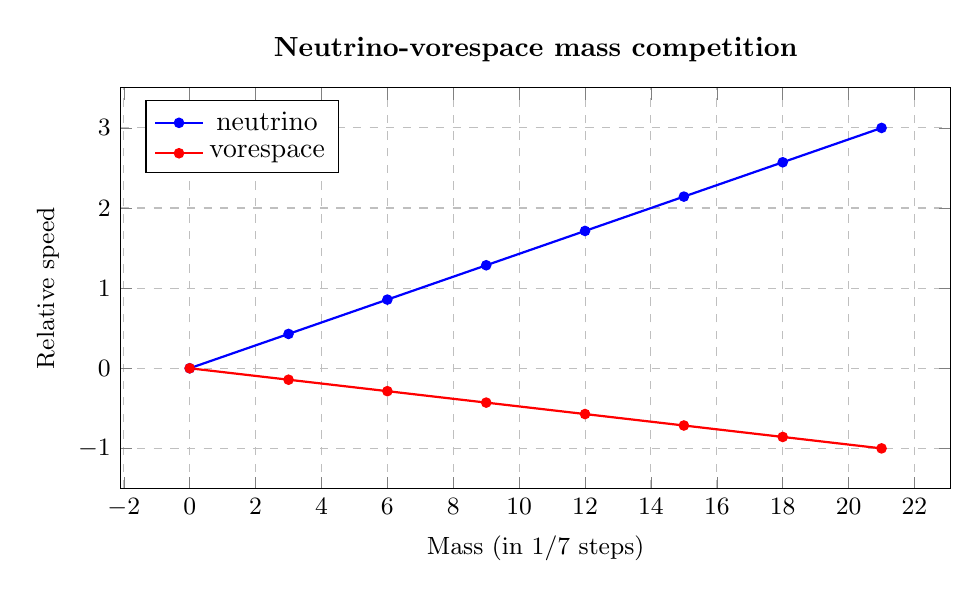
\begin{tikzpicture}
			\begin{axis}[
				width=\columnwidth,
				height=0.55\columnwidth,
				xlabel={Mass (in 1/7 steps)},
				ylabel={Relative speed},
				title={Neutrino-vorespace mass competition},
				xmajorgrids=true,
				ymajorgrids=true,
				grid style=dashed,
				ymin=-1.5,
				ymax=3.5,
				xlabel style={font=\small},
				ylabel style={font=\small},
				title style={font=\bfseries},
				tick label style={font=\small},
				legend pos=north west,
				]
				
				\addplot[
				color=blue,
				thick,
				mark=*, 
				mark size=1.5pt,
				] coordinates {
					(0,0)
					(3,3/7)
					(6,6/7)
					(9,9/7)
					(12,12/7)
					(15,15/7)
					(18,18/7)
					(21,21/7)
				};
				\addlegendentry{neutrino}
				\addplot[
				color=red,
				thick,
				mark=*, 
				mark size=1.5pt,
				] coordinates {
					(0,0)
					(3,-1/7)
					(6,-2/7)
					(9,-3/7)
					(12,-4/7)
					(15,-5/7)
					(18,-6/7)
					(21,-7/7)
				};   
				\addlegendentry{vorespace}
				
			\end{axis}
		\end{tikzpicture}
	\end{center}
	
	\begin{center}
		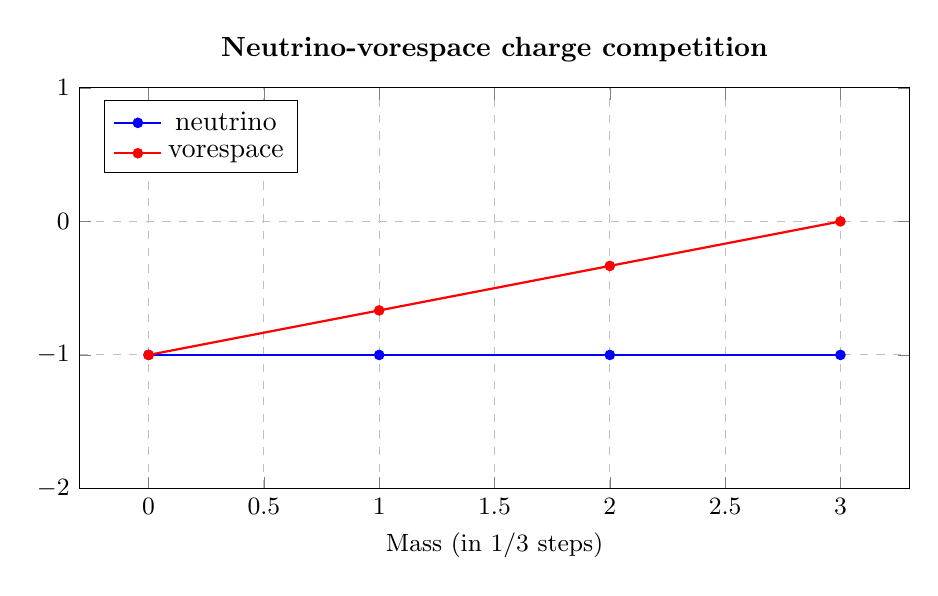
\begin{tikzpicture}
			\begin{axis}[
				width=\columnwidth,
				height=0.55\columnwidth,
				xlabel={Mass (in 1/3 steps)},
				title={Neutrino-vorespace charge competition},
				xmajorgrids=true,
				ymajorgrids=true,
				grid style=dashed,
				ymin=-2.0,
				ymax=1.0,
				xlabel style={font=\small},
				ylabel style={font=\small},
				title style={font=\bfseries},
				tick label style={font=\small},
				legend pos=north west,
				]
				
				\addplot[
				color=blue,
				thick,
				mark=*, 
				mark size=1.5pt,
				] coordinates {
					(0,-1)
					(7/7,-1)
					(14/7,-1)
					(21/7,-1)
				};
				\addlegendentry{neutrino}
				\addplot[
				color=red,
				thick,
				mark=*, 
				mark size=1.5pt,
				] coordinates {
					(0,-1)
					(7/7,-2/3)
					(14/7,-1/3)
					(21/7,0)
				};   
				\addlegendentry{vorespace}
				
			\end{axis}
		\end{tikzpicture}
	\end{center}
	
	Since a photon is an entropic revealer, it will be sensitive to the disparity of the internal states of each object and will not react in the same way depending on the states. It will cross the vorespace but will be blocked in the electron. The difference between the two is minimal—it is the fine-structure constant $\alpha$—but sufficient to change the rules of the game for the photon's interaction with $S_3$ type nodes.
	
	Now, mass is dual with the magnetic field: it is the flux $\Phi$ of electromagnetism. We can therefore see the distribution of mass values as a dual distribution of magnetic charge values of the associated monopole. By normalizing the charges to positive values, we have:
	
	\begin{center}
		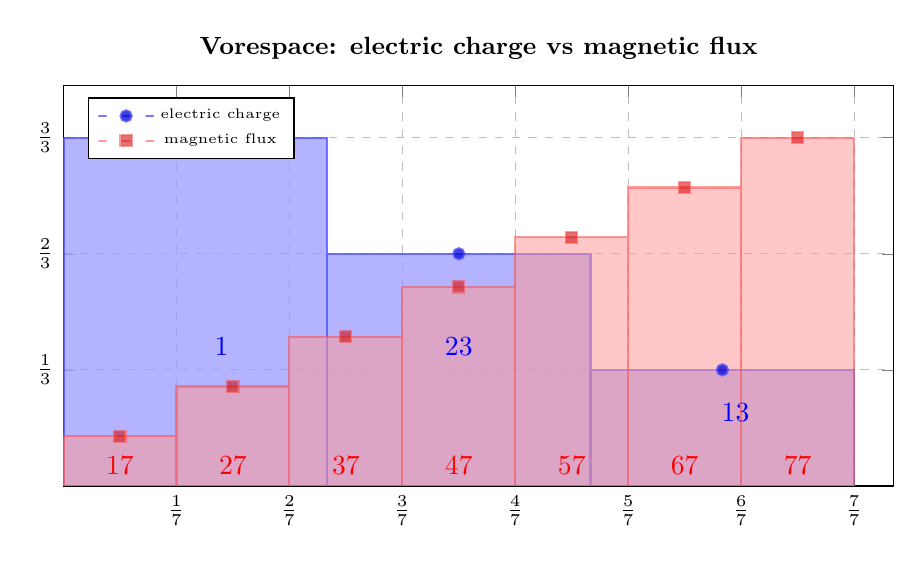
\begin{tikzpicture}
			\begin{axis}[
				width=\columnwidth,
				height=0.55\columnwidth,
				xmin=0, xmax=1.05,
				ymin=0, ymax=1.15,
				grid style=dashed,
				title={Vorespace: electric charge vs magnetic flux},
				grid=major,
				legend pos=north west,
				legend style={font=\tiny},
				title style={font=\bfseries\small},
				xtick={1/7,2/7,3/7,4/7,5/7,6/7,7/7},
				xticklabels={
					\( \frac{1}{7} \), \( \frac{2}{7} \), \( \frac{3}{7} \), 
					\( \frac{4}{7} \), \( \frac{5}{7} \), \( \frac{6}{7} \), \( \frac{7}{7} \)
				},
				xticklabel style={font=\small},
				ytick={1/3, 2/3, 3/3},
				yticklabels={
					\( \frac{1}{3} \), \( \frac{2}{3} \), \( \frac{3}{3} \), 
				},
				yticklabel style={font=\small}, 
				]
				\addplot+[ybar, bar width=1/3, fill=blue!40, draw=blue!70, thick, opacity=0.75] 
				coordinates {
					(1/6,  1)   
					(1/2,  2/3)   
					(5/6,  1/3)     
				};
				\addplot+[ybar, bar width=1/7, fill=red!40, draw=red!70, thick, opacity=0.55] 
				coordinates {
					(1/14, 1/7)
					(3/14, 2/7)
					(5/14, 3/7)
					(7/14, 4/7)
					(9/14, 5/7)
					(11/14,6/7)
					(13/14,1)
				};
				\legend{electric charge, magnetic flux};
				\node[color=red] at (2/28, 0.06) {\R{1}{7}};
				\node[color=red] at (6/28, 0.06) {\R{2}{7}};
				\node[color=red] at (10/28, 0.06) {\R{3}{7}};
				\node[color=red] at (14/28, 0.06) {\R{4}{7}};
				\node[color=red] at (18/28, 0.06) {\R{5}{7}};
				\node[color=red] at (22/28, 0.06) {\R{6}{7}};
				\node[color=red] at (26/28, 0.06) {\R{7}{7}};
				\node[color=blue] at (0.2, 0.4) {1};
				\node[color=blue] at (0.5, 0.4) {\R{2}{3}};
				\node[color=blue] at (0.85, 0.21) {\R{1}{3}};
			\end{axis}
		\end{tikzpicture}
	\end{center}
	
	\begin{center}
		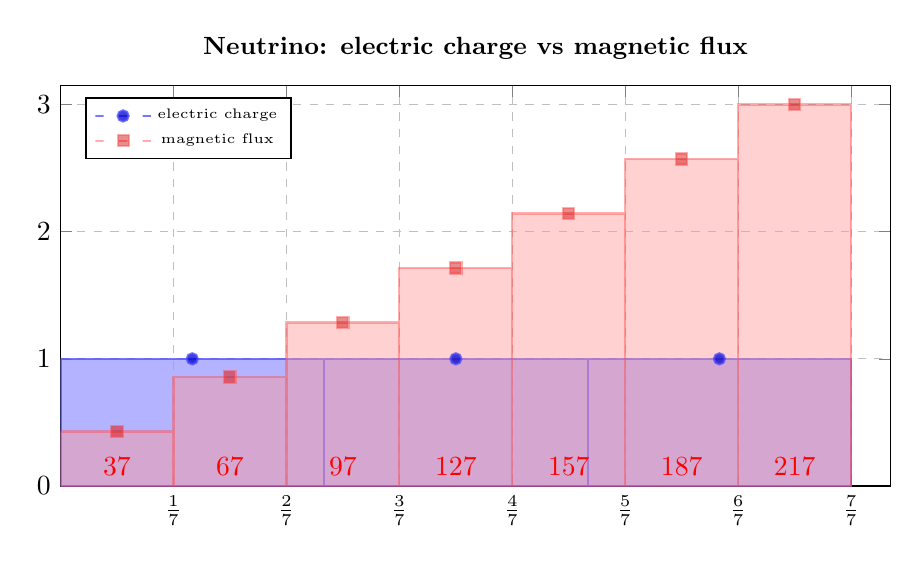
\begin{tikzpicture}
			\begin{axis}[
				width=\columnwidth,
				height=0.55\columnwidth,
				xmin=0, xmax=1.05,
				ymin=0, ymax=3.15,
				grid style=dashed,
				title={Neutrino: electric charge vs magnetic flux},
				grid=major,
				legend pos=north west,
				legend style={font=\tiny},
				title style={font=\bfseries\small},
				xtick={1/7,2/7,3/7,4/7,5/7,6/7,7/7},
				xticklabels={
					\( \frac{1}{7} \), \( \frac{2}{7} \), \( \frac{3}{7} \), 
					\( \frac{4}{7} \), \( \frac{5}{7} \), \( \frac{6}{7} \), \( \frac{7}{7} \)
				},
				xticklabel style={font=\small},
				]
				\addplot+[ybar, bar width=1/3, fill=blue!40, draw=blue!70, thick, opacity=0.75] 
				coordinates {
					(1/6,  1)   
					(1/2,  1)   
					(5/6,  1)     
				};
				
				\addplot+[ybar, bar width=1/7, fill=red!40, draw=red!70, thick, opacity=0.45] 
				coordinates {
					(1/14, 3/7)
					(3/14, 6/7)
					(5/14, 9/7)
					(7/14, 12/7)
					(9/14, 15/7)
					(11/14,18/7)
					(13/14,21/7)
				};
				\legend{electric charge, magnetic flux};
				\node[color=red] at (2/28, 0.15) {\R{3}{7}};
				\node[color=red] at (6/28, 0.15) {\R{6}{7}};
				\node[color=red] at (10/28, 0.15) {\R{9}{7}};
				\node[color=red] at (14/28, 0.15) {\R{12}{7}};
				\node[color=red] at (18/28, 0.15) {\R{15}{7}};
				\node[color=red] at (22/28, 0.15) {\R{18}{7}};
				\node[color=red] at (26/28, 0.15) {\R{21}{7}};    
			\end{axis}
		\end{tikzpicture}
	\end{center}
	
	For the vorespace, the magnetic charge is induced: it is the result of the presence of an electric charge. Conversely, for the neutrino, the magnetic charge is intrinsic and the electric charge is induced. The neutrino is the only true magnetic monopole\footnote{A new approach to capturing neutrinos would be to deflect them in a magnetic field.}.
	
	It is not necessary, as with Dirac's magnetic monopole, to invent some "Dirac string" to describe the monopole's field, because the charge (magnetic) phonon, in every respect equivalent to the mass phonon, fully describes the field.
	
	Here, the flux varies by whole steps. We thus have:
	
	\begin{equation*}
		\Phi_m = \sum_{i=1}^{7} \vec{B_i} \cdot \vec{S_i} = \mu_0 q_m
	\end{equation*}
	thus
	\begin{equation*}
		B_i S_i = \mu_0 q_{m_i}
	\end{equation*}
	
	Now, the blade surfaces vary proportionally according to a ratio of \R{1}{7}:
	\begin{equation*}
		S_i = \frac{i}{7} S_0 = \frac{i}{7} \pi \frac{L_p^2}{2}
	\end{equation*}
	
	hence
	\begin{equation*}
		q_{m_i} \mu_0 = \frac{i}{7} B_i S_0
	\end{equation*}
	
	Thus
	\begin{equation*}
		\left\{
		\begin{split}
			\mu_0  &\propto S_0  \\ 
			q_{m_i}&\propto \frac{i}{7} B_i 
		\end{split}
		\right.
	\end{equation*}
	
	The magnetic permeability is indeed proportional to the blade surface, and the magnetic charge is quantized. Unsurprisingly, we recover Dirac's quantization of magnetic charge, the measurements of the quantum Hall effect \cite{klitzing1980new}, and the solution found is close to the Chern-Simons soliton \cite{jackiw1990solitons}.
	
	\begin{center}
		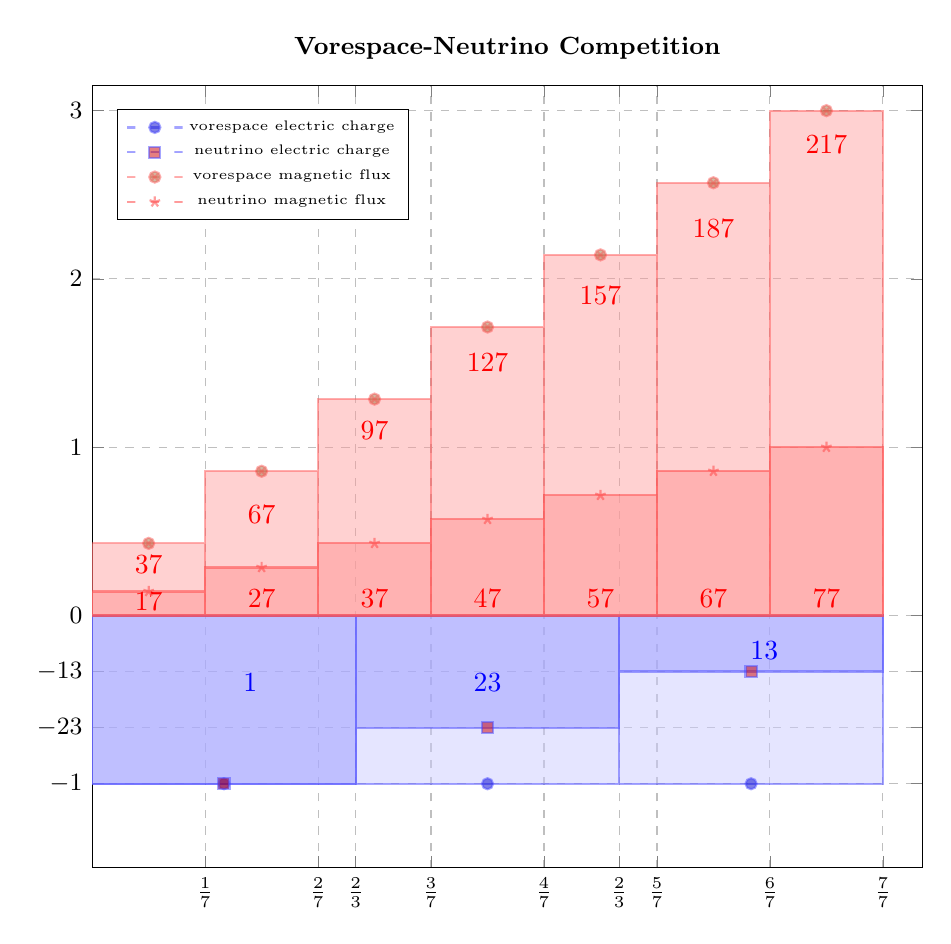
\begin{tikzpicture}
			\begin{axis}[
				width=\columnwidth,          % <-- exact page width
				height=0.95\columnwidth,     % proportional height
				xmin=0, xmax=1.05,
				ymin=-1.5, ymax=3.15,
				grid style=dashed,
				%xlabel={Position \( x \)},
				%ylabel={Height},
				title={Vorespace-Neutrino Competition},
				grid=major,
				legend pos=north west,
				legend style={font=\tiny},
				title style={font=\bfseries\small},
				xtick={1/7,2/7,1/3,3/7,4/7,2/3,5/7,6/7,7/7},
				xticklabels={
					\( \frac{1}{7} \), \( \frac{2}{7} \), \( \frac{2}{3} \), \( \frac{3}{7} \), 
					\( \frac{4}{7} \), \( \frac{2}{3} \), \( \frac{5}{7} \), \( \frac{6}{7} \), 
					\( \frac{7}{7} \)
				},
				xticklabel style={font=\small},
				ytick={-1, -2/3, -1/3, 0, 1, 2, 3},
				yticklabels={
					\( -1 \),     \( \Ru{-}{2}{3}{} \), \( \Ru{-}{1}{3}{} \),
					\( 0 \),  \( 1 \), \( 2 \), \( 3 \),
				},
				yticklabel style={font=\small},    
				]
				% ==================== Series 1/3: wide bars (width = 1/3) ====================
				\addplot+[ybar, bar width=1/3, fill=blue!20, draw=blue!70, thick, opacity=0.5] 
				coordinates {
					(1/6,  -1)   % center of the first bar
					(1/2,  -1)   % center of the second bar
					(5/6,  -1)     % center of the third bar            
				};
				\addplot+[ybar, bar width=1/3, fill=blue!40, draw=blue!70, thick, opacity=0.5] 
				coordinates {
					(1/6,  -1)   % center of the first bar
					(1/2,  -2/3)   % center of the second bar
					(5/6,  -1/3)     % center of the third bar
				};
				% ==================== Series 1/7: narrow bars (width = 1/7) ====================
				\addplot+[ybar, bar width=1/7, fill=red!40, draw=red!70, thick, opacity=0.45] 
				coordinates {
					(1/14, 3/7)
					(3/14, 6/7)
					(5/14, 9/7)
					(7/14, 12/7)
					(9/14, 15/7)
					(11/14,18/7)
					(13/14,21/7)
				};
				\node[color=red] at (2/28, 0.3) {\R{3}{7}};
				\node[color=red] at (6/28, 0.6) {\R{6}{7}};
				\node[color=red] at (10/28, 1.1) {\R{9}{7}};
				\node[color=red] at (14/28, 1.5) {\R{12}{7}};
				\node[color=red] at (18/28, 1.9) {\R{15}{7}};
				\node[color=red] at (22/28, 2.3) {\R{18}{7}};
				\node[color=red] at (26/28, 2.8) {\R{21}{7}};    
				% == vorespace ==
				\addplot+[ybar, bar width=1/7, fill=red!40, draw=red!70, thick, opacity=0.55] 
				coordinates {
					(1/14, 1/7)
					(3/14, 2/7)
					(5/14, 3/7)
					(7/14, 4/7)
					(9/14, 5/7)
					(11/14,6/7)
					(13/14,1)
				};
				\legend{vorespace electric charge, neutrino electric charge, vorespace magnetic flux, neutrino magnetic flux, };
				\node[color=red] at (2/28, 0.08) {\R{1}{7}};
				\node[color=red] at (6/28, 0.1) {\R{2}{7}};
				\node[color=red] at (10/28, 0.1) {\R{3}{7}};
				\node[color=red] at (14/28, 0.1) {\R{4}{7}};
				\node[color=red] at (18/28, 0.1) {\R{5}{7}};
				\node[color=red] at (22/28, 0.1) {\R{6}{7}};
				\node[color=red] at (26/28, 0.1) {\R{7}{7}};
				\node[color=blue] at (0.2, -0.4) {1};
				\node[color=blue] at (0.5, -0.4) {\R{2}{3}};
				\node[color=blue] at (0.85, -0.21) {\R{1}{3}};
			\end{axis}
		\end{tikzpicture}
	\end{center}
	
	How can we now determine the fine-structure constant? We note two unsettling facts. First, the value of this constant is surprisingly close to the neutrino mass ($7.2 \cdot 10^{-3}$ vs $7.6 \cdot 10^{-3}$). Furthermore, the fine-structure "constant" is not constant. It varies logarithmically, increasing for the Z boson \cite{workman2022review}. If we extrapolate the experimental measurements of the electron and Z boson constants\footnote{Taking $\alpha_{e^-}=7.297 \cdot 10^{-3}$ and $\alpha_{Z}=7.815 \cdot 10^{-3}$, we obtain the line $y=6.475 \cdot 10^{-5}\log_2{x}+5.743 \cdot 10^{-3}$, where $\log_2$ is the base-2 logarithm.} by plotting a logarithmic curve, we obtain:
	
	\begin{center}
		\begin{tikzpicture}
			\begin{axis}[
				xmode=log,
				log basis x=2,                  % log scale in base 2
				xmin=2^0, xmax=2^36,           % x range
				ymin=0.0055, ymax=0.0082,
				xlabel={Nodes},
				ylabel={},
				title={Fine-Structure Constants\\ (logarithmic scale)},
				grid=major,
				xmajorgrids=true,
				ymajorgrids=true,
				grid style=dashed,
				title style={align=center, font=\bfseries},
				width=0.95\columnwidth,          % <-- exact page width
				height=0.55\columnwidth,     % proportional height
				xtick={2^0, 2^8, 2^16, 2^24, 2^32, 2^36},
				xticklabels={
					\(\underset{neutrino}{1}\), \(8\), \(16\), 
					\(\underset{electron}{24}\), \(\underset{Z\ boson}{32}\), \(36\),
				},
				xticklabel style={font=\small},
				ytick={ 0.005, 0.006, 0.007, 0.008},
				yticklabels={
					\(0.005\), \(0.006\), 
					\(0.007\), \(0.008\),
				},
				yticklabel style={font=\small},
				scaled y ticks=false,
				]
				\addplot[blue, thick, domain=2^0:2^32] 
				{6.25e-5 * log2(x) + 0.0058};
				\addplot[blue, only marks, mark=*, mark size=1.5pt] 
				coordinates {
					(2^0, {0.0000625 * log2(2^0) + 0.0058})
					(2^8, {0.0000625 * log2(2^8) + 0.0058})
					(2^16, {0.0000625 * log2(2^16) + 0.0058})
					(2^24, {0.0000625 * log2(2^24) + 0.0058})
					(2^32, {0.0000625 * log2(2^32) + 0.0058})
				};
			\end{axis}
		\end{tikzpicture}
	\end{center}
	
	There is thus one constant per node of the plenum (with the neutrino constant being approximately $5.743 \cdot 10^{-3}$, or roughly $1/174$), which is not extraordinary in itself, as the constant measures the effect of mass (or magnetism) of a node's constituents relative to the vorespace model (which is only electrically charged). That the effect follows a logarithmic law is therefore intrinsic to \PQ.
	
	Let us look at how these constants evolve by calculating their approximate values from the experimentally determined line.
	
	%\vspace*{-0.5cm}
	\begin{center}
		\begin{longtblr}[
			caption={\footnotesize{\textbf{Calculation of approximate values of fine-structure constants}}},
			label = {tblr:5-0-3},
			]{
				colspec={Q[c,m]  Q[2.2cm,c,m] Q[3.5cm,c,m] },
				rowspec={Q[c,m]},
				row{odd}={bg=blue!10!white},
				row{1}={c,mode=text,fg=white,bg=pkcolor, cmd=\textbf},
				rowsep=2pt, colsep=3pt,
				vline{2-Y} = {1}{0.3pt,gray!50},
				vline{2-Y} = {2-Z}{0.3pt,gray!30},
				hline{Z} = {0.1pt,blue},
				rowhead = 1, 
			}        
			Nodes  &   $\alpha$               &  Ratio (approximate)   \\
			1    & 5.743$\cdot 10^{-3}$     &      1/174                  \\
			8    & 6.261$\cdot 10^{-3}$     &      1/160                  \\ 
			16    & 6.779$\cdot 10^{-3}$     &      1/148                  \\ 
			24    & 7.297$\cdot 10^{-3}$     &      1/137                  \\
			32    & 7.815$\cdot 10^{-3}$     &      1/125                  \\
			40    & 8.333$\cdot 10^{-3}$     &      1/120                  \\
			48    & 8.851$\cdot 10^{-3}$     &      1/113                  \\
			56    & 9.369$\cdot 10^{-3}$     &      1/107                  \\
			64    & 9.887$\cdot 10^{-3}$     &      1/101                  \\          
		\end{longtblr}
	\end{center}
	
	We "feel" therefore that there exists a logarithmic construction law based on $2^8$, and we also "feel" that this law acts fractally, first within the node, then in the series of nodes. Extrapolating it externally is not costly, as it is very Ockhamian.
	
	By calculating the ratios of two consecutive fine-structure constants, we realize that the value varies very little, likely due only to previous approximations. It is therefore judicious to choose the value corresponding to known variables, such as the electron and the Z boson, which yields a value of approximately $1.07$, or $1 + \R{7}{100}$. Calling this value $\Phi$, we deduce the logarithmic variation law of the fine-structure constants:
	\begin{equation}
		\label{eq:structure-fine}
		\alpha_{S_i} = \Phi^i \alpha_{S_0}, \text{ with } i \text{ varying from 0 to 8.} 
	\end{equation}
	
	Let us study the action of the vorespace and the neutrino. Dimensionally, the action of systems follows the product of the electric charge and the magnetic charge (Weber $\times$ Coulomb, i.e., $Wb\cdot C=V\cdot s \cdot A \cdot s = kg \cdot m^2 \cdot s = J \cdot s$). We can thus plot the evolution of the actions, considering that the magnetic charge is proportional to the flux (and thus that the scale of the neutrino action is not respected):
	
	%\clearpage
	\begin{center}
		\begin{longtblr}[
			caption={\footnotesize{\textbf{Actions of vorespace and neutrino}}},
			label = {tblr:10-0-2},
			note{a}  = {up to a multiplicative constant.},
			]{
				colspec={Q[c,m] Q[3.5cm, c,m] Q[3.5cm,c,m] },
				rowspec={Q[c,m]},
				row{odd}={bg=blue!10!white},
				row{1}={c,mode=text,fg=white,bg=pkcolor, cmd=\textbf},
				rowsep=2pt, colsep=3pt,
				vline{2-Y} = {1}{0.3pt,gray!50},
				vline{2-Y} = {2-Z}{0.3pt,gray!30},
				hline{Z} = {0.1pt,blue},
				rowhead = 1,
			}        
			Step       &    Vorespace     &  Neutrino \TblrNote{a}   \\
			\R{1}{7}  &    \R{1}{7}     &   \R{3}{7}  \\
			\R{2}{7}  &    \R{2}{7}     &   \R{6}{7}  \\
			\R{3}{7}  &    \R{5}{63}    &   \R{9}{7}  \\
			\R{4}{7}  &    \R{8}{21}    &   \R{12}{7} \\
			\R{5}{7}  &    \R{5}{63}    &   \R{15}{7} \\
			\R{6}{7}  &    \R{2}{7}     &   \R{18}{7} \\
			\R{7}{7}  &    \R{2}{21}    &   \R{21}{7} \\                
		\end{longtblr}
	\end{center}
	\begin{center}
		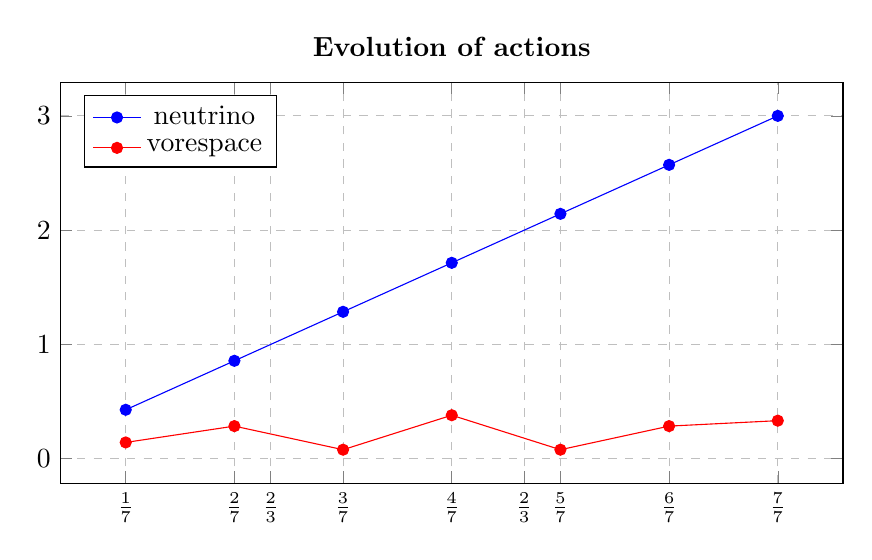
\begin{tikzpicture}
			\begin{axis}[
				xlabel={},
				ylabel={},
				title={Evolution of actions},
				grid=major,
				xmajorgrids=true,
				ymajorgrids=true,
				grid style=dashed,
				title style={align=center, font=\bfseries},
				width=0.95\columnwidth,          % <-- exact page width
				height=0.55\columnwidth,     % proportional height
				legend pos=north west,
				xtick={1/7,2/7,1/3,3/7,4/7,2/3,5/7,6/7,7/7},
				xticklabels={
					\( \frac{1}{7} \), \( \frac{2}{7} \), \( \frac{2}{3} \), \( \frac{3}{7} \), 
					\( \frac{4}{7} \), \( \frac{2}{3} \), \( \frac{5}{7} \), \( \frac{6}{7} \), 
					\( \frac{7}{7} \)
				},
				xticklabel style={font=\small},
				]
				\addplot[blue, mark=*,] 
				coordinates {
					(1/7, 3/7)
					(2/7, 6/7)
					(3/7, 9/7)
					(4/7, 12/7)
					(5/7, 15/7)
					(6/7, 18/7)
					(7/7, 21/7)
				};
				\addplot[red, mark=*,]
				coordinates {
					(1/7, 1/7)
					(2/7, 2/7)
					(3/7, 5/63)
					(4/7, 8/21)
					(5/7, 5/63)
					(6/7, 2/7)
					(7/7, 7/21)
				} ;
				\legend{neutrino, vorespace};
			\end{axis}
		\end{tikzpicture}
	\end{center}
	
	It follows that, within the framework of the magnetic monopole, the action varies by integer steps:
	\begin{equation*}
		q_e q_m \propto i, \text{ with } i \text{ varying from 1 to 7.} 
	\end{equation*}
	
	The process being fractal, its properties are scale-invariant. We can thus find the proportion factor by studying any similar node, in particular the electron. Now, we have seen that the energy over a complete cycle was a photon of energy $h$, hence an action $h$ over one cycle. Here, it is a matter of reducing the cycle to the electron alone, thus over a half-cycle. We therefore have
	\begin{equation*}
		q_e q_m = i\frac{h}{2}, \ \text{ with } i \text{ varying from 1 to 7.} 
	\end{equation*}
	
	It follows that the first magnetic dipole is the neutrino-antineutrino association. The coupling of the two charge phonons loops upon itself, creating the first bipolar magnetic field.
	
	Obviously, this structure is highly unstable and the first stable node that keeps the bipolar magnetic field invariant is the $S_1$ node. The second node of the same kind is the $S_4$, the Z boson. These two nodes are the hopfions described on page~\pageref{figure:1-hopfion} in figure~\ref{figure:1-hopfion}. We can now greatly improve their representation by drawing a torus of turbines instead of the simple torus in figure~\ref{figure:1-hopfion}. In the macroscopic world, magnetic particles are of course composite.
	
	One must clearly differentiate the magnetic fields under discussion. The magnetic monopole creates a field $\vec{H}$ with a central potential. $S_3$-type nodes, which are electric monopoles, generate induced magnetic fields $\vec{B}$. All other nodes generate magnetic fields $\vec{H}$, but these are magnetic bipoles, thus with closed field lines. All this can be summarized in table \ref{tblr:11-0-2}:
	\end{multicols}
	\vspace*{-1.0cm}
	\begin{center}
	\begin{longtblr}[
		caption={\footnotesize{\textbf{Electromagnetic structure of nodes}}},
		label = {tblr:11-0-2},
		]{
			colspec={Q[2cm,c,m] Q[2.8cm,c,m] Q[2.8cm,c,m] Q[2.8cm,c,m] Q[2.8cm,c,m]},
			rowspec={Q[c,m]},
			row{odd}={bg=blue!10!white},
			row{1}={c,mode=text,fg=white,bg=pkcolor, cmd=\textbf},
			rowsep=2pt, colsep=3pt,
			vline{2-Y} = {1}{0.3pt,gray!50},
			vline{2-Y} = {2-Z}{0.3pt,gray!30},
			hline{Z} = {0.1pt,blue},
			rowhead = 1,
		}        
		Node        &Electric monopole &Magnetic monopole&Magnetic dipole& Magnetic field \\
		$S_0(-1,0)$ &    \vraiV          &   \fauxR          &    \fauxR       &       $\vec{B}$  \\
		$S_0(0,1) $ &    \fauxR          &   \vraiV          &    \fauxR       &       $\vec{H}$  \\
		$S_1(0,1) $ &    \fauxR          &   \fauxR          &    \vraiV       &       $\vec{H}$  \\
		$S_2(0,1) $ &    \fauxR          &   \fauxR          &    \vraiV       &       $\vec{H}$  \\
		$S_3(-1,1)$ &    \vraiV          &   \fauxR          &    \fauxR       &       $\vec{B}$  \\
		$S_4(0,1) $ &    \fauxR          &   \fauxR          &    \vraiV       &       $\vec{H}$  \\
		$S_5(0,1) $ &    \fauxR          &   \fauxR          &    \vraiV       &       $\vec{H}$  \\
		$S_6(-1,1)$ &    \vraiV          &   \fauxR          &    \fauxR       &       $\vec{B}$  \\
	\end{longtblr}
	\end{center}
	
	\begin{multicols}{2}
	Since
	\begin{equation*}
		\begin{split}
			[q_e q_m] &= [ \text{Action} ]                         \\
			&= [\text{Angular momentum}]                 \\
			&= [\text{Rotational angular}              \\
			&\phantom{= [} \ \text{momentum}] \\
		\end{split}
	\end{equation*}
	and by bringing together the action of the nodes and magnetism, it follows that spin is \textit{the expression of the magnetic moment of $S_3$-type nodes}. It is therefore linked both to the presence of electric charge and to the shape of the blades, their width (the bi-vector), and their thickness (tri-vector).
	
	
	\begin{mybox}[breakable,colback=blue!10, colbacktitle=pkcolor]{Spin}
		Spin is not a property that emerged \textit{ex nihilo} from the quantum dimension. It is the expression of the magnetic moment induced by the excitation of the electric charge of an $S_3$-type node.
	\end{mybox}
	
	We thus have
	\begin{equation*}
		S = q_e q_m = n \frac{h}{2}, \text{ with } n \text{ varying from 1 to 7.} 
	\end{equation*}
	
	Finally, spin being both collinear and proportional to the flux, and a multiple of electric and magnetic charge, it is therefore the \textit{Poynting vector} at the level of the $S_3$ node:
	\begin{equation*}
		\vec{S} = \vec{E} \wedge \vec{H} 
	\end{equation*}
	
	Spin is thus the \textit{magnetic flux density}, that is, \textit{the power of magnetic radiation}, whose origin can be electric (vorespace, electron) or purely magnetic as with the magnetic dipole that is the neutrino. Regardless, it arises from the rotation of a node and is thus closely linked to this movement. We will call the angular momentum due to rotation the \textit{orbital} angular momentum $\vec{L}$. $\vec{S}$ and $\vec{L}$ are thus the two sides of the same movement: on one side the electric charge, on the other the induced magnetic field.
	
	The orbital angular momentum $\vec{L}$ corresponding to the charge, it necessarily rotates by integer values of a turn. It thus varies by natural integer steps. We will call $l$ the value of this momentum.
	
	One can be convinced of this by returning to the definition of angular momentum:
	\begin{equation*}
		\vec{L} = \vec{r} \wedge \vec{p} 
	\end{equation*} 
	or
	\begin{equation*}
		l = m r^2 \omega = 2n \pi m r^2 
	\end{equation*}
	with $n$ the number of turns and $r$ the radius of the blade, which therefore depends on the size of the $S_i$ node: $r=r(i)$.
	
	The rotation of the blades also induces a purely magnetic angular momentum $\vec{\mathcal{M}}$, collinear with the orbital angular momentum, of which it is in some sense the dual. $\vec{\mathcal{M}}$ is thus proportional to $\vec{L}$. It is trivial to show that the proportionality factor corresponds to the gyroscopic ratio $\gamma = q_e/2m$, with the classical calculation and approach being applicable here.
	
	We therefore have
	\begin{equation*}
		\vec{\mathcal{M}} = \frac{q_e}{2m} \vec{L} 
	\end{equation*} 
	\vfill\strut
	
	\begin{figure}[H]
		\label{figure:Moment-0}
		\centering
		
\includegraphics[width=0.8\columnwidth]{moments-cinetiques.pdf}
		\caption{\footnotesize{\textbf{Angular momenta of the blades.} The blade (in light brown) makes an angle with the vertical (represented by the $(Oz)$ axis), a mark of electric charge. The orbital angular momentum $\vec{L}$ is perpendicular to the blade, while the magnetic angular momentum, assimilated to the magnetic moment, in green, is collinear to it. In orange, the flux at a given location therefore depends on the radius. Spin is the magnetic flux density -- the Poynting vector -- thus the average of the flux over the blade's surface. The flux, as well as the spin, is perpendicular to the surface. The figure is not to scale.}}
	\end{figure}
	
	One must remember that the blade is a helicoid blade and that it is better represented as follows (up to variable thickness):
	\begin{center}
		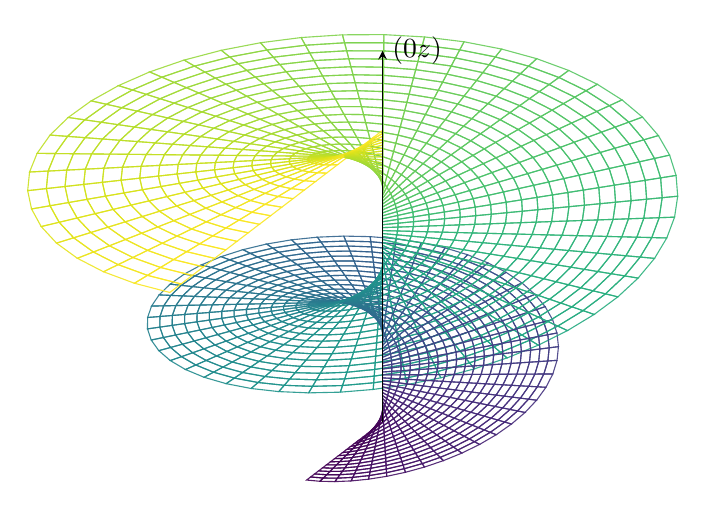
\begin{tikzpicture}
			\def\a{0.2}
			\def\b{0.25}
			\begin{axis}[
				view={120}{30},     % View angle
				width=\columnwidth, height=\columnwidth,
				axis lines=none,    % Hide axes
				xmin=-8, xmax=2,
				ymin=-7, ymax=5,
				zmin=-1, zmax=4,
				colormap/viridis,
				]
				\addplot3 [
				mesh,               % wireframe
				shader=interp,      
				opacity=0.9,        
				domain=0:4*pi,      
				domain y=0:2.5,     
				samples=100,         
				samples y=20,
				] (
				{(1 + (1/7)*x)*y*cos(deg(x))},    
				{(1 + (1/7)*x)*y*sin(deg(x))},    
				{\b*x}
				);
				\draw[thin, -stealth] (axis cs:0,0,0) -- (axis cs:0,0,4) node[right] {$(0z)$};
			\end{axis}
		\end{tikzpicture}
	\end{center}
	
	\MQ\ has chosen to consider the set $\vec{S}+\vec{L}$ as characteristic of the quantum object. In reality, spin is not totally independent of the intrinsic magnetic angular momentum, as it is the sum of it over 2 turns.
	
	Indeed, if we consider the node from an energetic point of view, thus of work, we have
	\begin{equation*}
		\left\{
		\begin{split}
			\delta W &= P(t) dt = S dt \\
			\delta W &= \mathcal{M} d\theta
		\end{split}
		\right.
	\end{equation*}
	or
	\begin{equation*}
		S = \mathcal{M} \frac{d\theta}{dt} = \mathcal{M} \omega
	\end{equation*}
	
	As the rotation speed of the vorespace is half that of the neutrino, we obtain for any massive particle:
	\begin{equation*}
		S = 2  \mathcal{M} \omega = 2 \frac{q_e}{2 m} = g \frac{q_e}{2 m}
	\end{equation*}
	
	The \textit{Lande factor}, emerged somewhat miraculously from the Dirac equations \cite{dirac1928quantum}, is in reality only the expression of the mass (and thus magnetism) of the particles being measured, i.e., massive particles.
	
	However, the measurement of the Lande factor shows that it is not rigorously equal to 2, but to 2 "plus one \R{2}{1000}." The neutrino thus rotates slightly faster than twice the speed of the vorespace. If the factor were exactly 2, it would be a fractal factor that would not change the properties of the vorespace, namely that the photon "passes through" the vorespace. But since the factor is very slightly larger, the geometry of the blade is very slightly modified, and the photon can no longer "pass through" the massive node: it will strike it, transferring its momentum, creating the electromagnetic interaction.
	
	Note that we could have directly intuited this result by simply saying that the vorespace flux is half that of the neutrino.
	
	Note finally that by choosing the projection of $\vec{L}$ as the magnetic quantum number, \MQ\ creates a confusion of genres. Certainly, orbital angular momentum is related to magnetism, in the sense that the latter is induced by rotation, but it would have been much more fortunate to name the quantum numbers $m_l$ as the projections of $\vec{\mathcal{M}}$. It may be very difficult to restore order due to habit. But the ease of understanding the underlying domains would have gained enormously...
	\medskip
	
	We can now link the Lande factor with the fine-structure constant. Consistent with \MQ\ calculations, the Lande factor corresponds to the enlargement of the magnetic circle. It is therefore the part of the excess radius, and we thus classically find that it is proportional to the fine-structure constant and that its proportion factor is the turn of a complete circle:
	\begin{equation*}
		g = \frac{\alpha}{2\pi}
	\end{equation*} 
	
	Mass, or magnetism, therefore induces a more subtle transformation than a simple widening of the blade surface and its thickness: it induces a swelling of the thickness that rounds off, somewhat on the model of an inner tube. This elongation, relative to the thickness, is exactly the Lande factor, roughly \R{2}{1000}.
	
	This surplus makes the passage of the photon impossible. Where it once passed by brushing against the vorespace, the extra thickness of the massive nodes blocks it, mechanically inducing an interaction between photons and $S_3$-type nodes.
	
	Furthermore, the blade radius being proportional to the node size, we find the logarithmic law of the fine-structure constant \eqref{eq:structure-fine}.
	
	Finally, the apparent speed of the neutrino, double that of the vorespace, should not hide that only the magnetic blade carries the real speed, i.e., triple that of the vorespace. The excess speed consequently applies only to this blade, which therefore rotates slightly faster than 3. For the electron, it rotates at $3.002\,319\,304$, or slightly more than 7\,\% over the theoretical speed. We find the jump of slightly more than \R{7}{100} stated in the fractal law.
	\medskip
	
	Unfortunately, I have not been able to calculate the exact value of $g$ (or $\alpha$). Either this requires a more astute mind, or this constant is intrinsic to the plenum, and is therefore the only true fine constant of the universe. The Big Bang model proposed below may lean in favor of this hypothesis: it would be the exact setting corresponding to the amount of energy necessary for the creation of the neutrino which allows for the development of the electromagnetic interaction in the universe.\footnote{The fact that this is the only rigorously undemonstrable "anomaly" bothers the author. All \PQ\ is structurally mechanical and explainable, and this should also be the case here. If it is true that it is impossible to calculate this constant, then it would indeed be the only fine-tuning of the universe.}
	
	\subsubsection{Other constants of physics}
	
	One should take the time to reconstruct all the constants of physics, even if, at this stage, one can very well reconstruct everything mechanically with those already found, as this is \textit{grosso modo} what current physics does.
	
	It should be noted that one constant has no real meaning: the Planck charge. It is a simple side effect of extrapolating Planck units to all characteristics of physics: by postulating a Planck charge and defining it as the elementary charge carried by a Planck particle—a particle of Planck size. We thus have a physical impossibility of representing such a particle, unless it is associated with two vorespaces or two neutrinos. The previous definition refers to the Schwarzschild radius, i.e., to the maximum mass of an object; therefore, it would rather be an assembly of neutrinos. However, by definition, neutrinos have no charge!
	
	\section{Equivalence of Quantum Plenodynamics with current physics}
	
	\subsection{Introduction} 
	
	It is necessary to ensure that \PQ\ is compatible with all of physics if it is to claim to be a physics of everything. It was built on mechanics and thermodynamics, as well as on electromagnetism. It is already compatible with these theories. However, it must still pass the test of the three great theories of physics: special and general relativity, and quantum mechanics.
	
	\subsection{Special Relativity}
	
	Regarding special relativity, this is the easiest part, because \PQ\ was built precisely by respecting the foundations of special relativity, namely a transfer of information based on the speed of light as the maximum speed.
	
	In a way, \PQ\ can be seen as the real counterpart of special relativity, which usually happens to be a general framework, valid everywhere. \PQ\ therefore embodies special relativity.
	
	It is easy to find the Lorentz factor in a moving particle. Its "caterpillar-like" evolution marks a difference between the start of its displacement and the end, which can be triangularized in a right-angled triangle, allowing the extraction of the Lorentz factor.
	
	Time does not dilate strictly speaking, but the re-attachment time of the caterpillar lengthens, as the path to be traveled becomes increasingly large.
	
	Similarly, the tension in the caterpillar increases with speed, which in return results in an increase in mass, proportional to this tension.
	
	\PQ\ is therefore fully compatible with special relativity: one can even say that \PQ\ \textbf{is} special relativity.
	
	\subsection{General Relativity}
	
	Part of the work has also already been carried out within the framework of general relativity. Thus, in Einstein's theory, a mass curves spacetime; in \PQ, a mass acts on the plenum by imprinting a shear wave upon it, the mass phonon.
	
	Where Einstein shows that light follows a geodesic of spacetime, the photon of the plenum follows the mass phonon as an entropic surfer. It moves up the entropy thalwegs, which lead toward the masses.
	
	In Einstein's spacetime, near a mass, time slows down. In the plenum, the mass phonon decreases the entropic transfer capacities, penalizing the transfer time: the more massive the phonon, the more the transfer time is penalized. Mass indeed acts as a time retarder around itself.
	
	Finally, general relativity postulates the equivalence between inertial mass and gravitational mass. In \PQ, gravitational mass is the mass of the vorespace, the tension that can be applied to a turbine. Inertial mass is that generated by the inertia of this vorespace. By construction, they are identical.
	
	\PQ\ is therefore fully compatible with general relativity.
	
	\subsection{Quantum Mechanics}
	
	\subsubsection{Introduction}
	
	We now enter the final stage. If we can prove the equivalence between \PQ\ and quantum mechanics, we will then have united the three great physics, and \PQ\ will definitively be compatible with a physics of everything.
	
	We will conclude this part with the construction of the atomic model according to the point of view of \PQ—a model that will allow not only for the modeling of the atom but also for explaining why it functions this way.
	
	\subsubsection{Wave-particle duality}
	
	It goes without saying that the phonon of mass and charge (if needed) around a particle constitutes the famous wave of quantum particles. It is no longer mysterious at all, since it is simply the interaction of a mass—a corpuscle, then—with the plenum.
	
	
	
	This wave nevertheless has interesting properties. It is a composite heptagonal standing wave, in the sense that it is simultaneously the sum of the waves of each of the particle's sub-nodes and the rotation of the particle itself.
	
	Thus, in the case of the electron for example, composed of $2^{24}$ neutrinos, it is the composition of $2^{24}$ heptagonal mini-waves mixed with a heptagonal wave of the electron itself. \textit{Technically, the wave is therefore not composed of an infinite number of waves, but of a finite number.} Of course, the composition makes this number "large enough," which makes the "infinite" approximation acceptable as a first step.
	
	Note that the wave entirely defines the position of the particle. One could study only the wave and account for the characteristics of the particle. From this point of view, the wave indeed "pilots" the particle, which was Louis de Broglie's point of view.\cite{debroglie1924recherches}
	
	However, it is indeed the particle that gives rise to the wave, and it is more accurate to say that \textit{the particle pilots the wave}. It is therefore not \textit{stricto sensu} a pilot-wave, but rather a \textbf{pilot-particle}, if we want to keep Louis de Broglie's terminology.
	
	Note a major difference between the two theories: determinism is absolute in \PQ. It "suffices" to calculate what the wave looks like to determine what the particle looks like, and vice versa: since one and the other are in a relationship of total equivalence—in bijection, mathematicians would say—knowing one is enough to know everything about the other.
	
	This equivalence answers the great quantum question of what exactly the wave function represents. The Copenhagen school asserts that it contains the seeds of everything that can be known about the properties of the quantum particle. This is correct, in the sense that it is generated by the quantum particle in question, according to a deterministic relationship that takes into account all its states. Quantum mechanics takes this wave function as the reference for information, whereas the real reference is the particle. In a way, quantum mechanics follows an object lit by the sun by following its shadow. When quantum mechanics measures the shadow, it then turns its gaze toward the object and claims that the shadow has transformed—collapsed—into the object. In reality, \textit{quantum measurement is just a change of point of view.}
	
	Finally, we saw earlier that wave-particle duality and the quantization of momentum mechanically led to de Broglie's formula.
	
	\subsubsection{The case of the photon}
	
	The photon, our entropic surfer, poses a real problem. By construction, it is only a wave. Duality does not apply to its case, which is bothersome, to say the least, for Albert Einstein, who received his Nobel Prize after explaining the threshold of the photoelectric effect by the presence of light corpuscles!
	
	Indeed, \PQ\ fully assumes changing the status of the photon in physics. Just as it explained the real nature and the origin of the photon, it assumes that the photon is only a pure wave.
	
	The question that then immediately arises is: how to explain that thousands of physics experiments over recent years highlight the dual nature of the photon? The answer is contained in the question: it is not the nature of the photon that the experiments measure, but... the instruments themselves. Thus, when a photon approaches a physical detector, the latter, by its atomic composition, influences the plenum by creating a mass phonon, and sometimes even a charge phonon. The photon, as a phonic surfer, immediately "obeys" the change in the plenum, creating the illusion that it too is endowed with a dual nature.
	
	This is perhaps the biggest revolution brought by \PQ: physicists have actually been measuring their instruments for years when they implement photons!
	
	\subsubsection{The role of measurement}
	
	This is a perfect transition to examine the role of measurement. Independently of the particular case of the photon, which is nonetheless the privileged actor of current experimental physics, one must look at the notion of measurement in general.
	
	In \MQ, measurement impacts the state of the system, reducing it to an eigenstate—the one measured. \MQ\ postulates that some state out of all the superimposed states was drawn by lot, according to true chance. The system is then irremediably reduced to the measured state.
	
	We saw above that, in reality, quantum measurement is a change of point of view. There is no collapse of the wave function, for the good reason that nature reveals the real, and the real is the object, not its relationship with the ether, even if this relationship can indirectly define it. It goes without saying that when physicists measure an electron, it is indeed the \node{$S_3(-1,1)$} object they expect to see and measure, not the heptagonal wave surrounding it, even if the latter is not without consequence for the measurement.
	
	We have indeed seen that measurement is not without impact at the level of \PQ. Indeed, measuring instruments, macroscopic by essence, have a direct impact on the plenum. \textit{They are therefore not neutral}. To truly experiment, the physicist must remove the bias introduced by the instrument itself. It will be complicated to completely free oneself from this bias when measuring quantum-sized objects.
	
	Take, for example, the classic case of electron interference through two slits. The electron possesses a wave, certainly. It can very advantageously interfere between two openings, forcing the electron's passage through one rather than the other.
	
	But what is the part of the mass phonon of each opening in this story? Around the two openings, two phonon corridors are created... Are we certain that each opening is atomically and rigorously the mirror of the other (otherwise, their mass phonon might differ and, thus, favor one measurement over another)? Furthermore, one must be certain to "hit right in the middle of the slits," because electron launching is deterministic in \PQ. That is to say, in theory, by launching the electrons identically, they should follow exactly the same trajectory and all pass through the same hole. Of course, any small thing along the trajectory is enough to change a micro-parameter and change the final result. And the surrounding air is full of interference!
	
	Of course, statistics often come to save the experiment: given the large number of uncontrollable parameters, it is reasonable to estimate that they statistically annihilate each other. One should therefore find experimental accuracy via statistics.
	
	Regardless, the question arises of what we are really measuring today in physics... at least at the quantum level when working on interference.
	
	It goes without saying that as soon as the mass or charge phonon can have an impact on any measurement, it must be taken into account, if only to gain some distance from the result.
	
	\subsubsection{Entanglement: the lure of chance}
	
	The famous EPR article\cite{einstein1935can} by Einstein, Podolsky, and Rosen launched a debate that ended recently, but which \PQ\ proposes to restart, with an unexpected conclusion. The experiment postulates that if \MQ\ is correct, then there exists a state of entanglement between two particles and that this state violates special relativity, since the information circulating between the two particles would circulate faster than the speed of light. Aspect's experiment\cite{aspect1982experimental} showed that this assertion was verified.
	
	Yet, \PQ\ asserts that determinism exists and that, in fact, entanglement does not exist. It is simply a side effect of quantum mechanics theory, which is not the simplest representation of reality, but a more complex theory, as mentioned by Poincaré\cite{poincare:1902:sh}.
	
	Quantum mechanics thus takes an indirect path to express quantum effects. The path of \PQ, being more direct, does not possess the side effects of quantum mechanics.
	
	Indeed, quantum mechanics hides what it does not know under the name of quantum chance. Not being able to calculate the real characteristics of a quantum particle, it has developed a divinatory technique—excellent, for that matter—to explain the behavior of quantum objects. But this technique postulates the idea of irreducible chance, therefore structural indeterminism, which is not a reflection of reality.
	
	Take the example of two electrons in a helium atom. They are entangled, in the sense that each has a spin opposite to the other. \MQ\ asserts that only measurement lifts this indeterminacy. In reality, there is no indeterminacy: each electron really possesses a spin opposite to the other. If you measure one, you do not change the value of the other. Entanglement is a consequence of the structure (which will be explained in the atomic model), not of measurement. Entanglement therefore does not exist from the point of view of quantum plenodynamics. You can move two entangled objects each to one end of the universe and measure one; no information will circulate to the other: both values are determined before the measurement.
	
	Thus, the EPR article, which supposed quantum mechanics was correct to postulate what followed, remains accurate: it is just that the starting hypothesis—the accuracy of \MQ—is not conformable to the real. Quantum mechanics uses a non-realistic chance that has consequences within quantum mechanics, not in reality. Entanglement exists in quantum mechanics, not in reality, because quantum mechanics does not represent the real, but a mathematical and complicated way to describe the real. This is a superb illustration of the dangers of using mathematics to describe physics, as stated by de Broglie\cite{debroglie1976physique}.
	
	So, how is it that Aspect's experiment is correct? For exactly the same reason that experiments on photons are correct: they do not measure entanglement \textit{in se}, but the interaction of photons with the instruments. To compensate for this interference from the sensors—here, waveplates—one would have to measure the photons with objects of the same nature as the photon itself. Quite a challenge!
	
	Regardless, this in no way detracts from Alain Aspect having achieved this extraordinary experiment.
	
	\subsubsection{The Pauli Exclusion Principle}
	
	The Pauli exclusion principle postulates that two fermions in the same place cannot have identical characteristics. This principle follows naturally from the $S_3$ structure of fermions which, to be together, must have compatible physical characteristics: for example, to assemble two $S_3$ nodes, one must be flipped, thus reversing its spin, so that the screwing directions are compatible. This principle is therefore structural in \PQ.
	
	We will see in the atomic model a finer reason for this principle, which actually results from the minimization of the energy of electrons in atomic orbits.
	
	\subsubsection{CPT Theorem}
	
	CPT conservation is structurally maintained in an $S_3$ node by the symmetry of the first 64 states and the following 64. Reversing chirality requires passing through all intermediate states. CPT symmetry is ensured by the turbine's structure.
	
	Regardless of the nodes, the 128-state structure is structurally compatible with CPT conservation.
	
	\subsubsection{The Heisenberg Uncertainty Principle}
	
	\PQ\ does not challenge the Heisenberg uncertainty principle. Indeed, the latter does not depend on the mathematical theory of quantum mechanics: it is an "obvious" observation that two linked characteristics cannot be measured at the same time, as the respective measurement times are not compatible with each other.
	
	Furthermore, the spatio-temporal quantization of the plenum makes the uncertainty principle trivial.
	
	\subsubsection{Conclusion on compatibility}
	
	\PQ\ and \MQ\ are therefore fully compatible. \PQ\ simply allows for a slight correction of \MQ, whose intrinsic chance led to conclusions that were sometimes... hazardous. Determinism regains its full rights in the quantum world, which is no longer bizarre, as quantum particles have regained a determined trajectory.
	
	\subsection{The atomic model}
	
	\subsubsection{Introduction}
	
	Until today, physics has observed that the atom exists and has deduced a model based on purely experimental data. It is a classic case of a "law" extrapolated from experimental observations\cite{poincare:1902:sh}. While the model is correct because it fits the experiment, it offers no explanation for "why" things function this way; in particular, it provides no answer to the \textbf{big question}: "why doesn't the electron fall into the nucleus?", a question that could be posed via its contrapositive version: "why does the electron orbit without spending energy?" \PQ\ proposes to resolve this enigma and to provide, for the first time, a consistent answer.
	
	Without going into details, the general idea of atomic construction is to find a natural stable state from elementary particles. The latter are only a step before the final stabilization, which is the atom. Stabilization in the plenum is always ensured by a node self-similar to $S_3$; thus, unsurprisingly, we will find this structure in the atom. The electron and the nucleus will play the role of the blades and "tangle" to form an $S_3$-type node. Of course, at this advanced stage of the particles, fusion will no longer be physically possible, and the $S_3$ node will be strongly distended: the electron and the nucleus will therefore no longer be stuck together.
	
	On the other hand, this spacing leaves free room to form a complex entanglement of $S_3$ nodes, where each added node will correspond to an atom in Mendeleev's table. Nature so much needs to embrace this $S_3$ node shape to stabilize itself that the entire set of electron shells itself forms an $S_3$-type node!
	
	So, ready for the journey to the heart of the atom? Let's go...
	
	\subsubsection{Foundations of the atomic nucleus}
	
	We saw that quarks, to converge toward a stable $S_3$-type node structure, associated in triplets to form a neutron and a proton.
	
	Technically, nature could have stopped there, but the presence of electrons will force neutrons and protons to find a common node shape for even more stability.
	
	One might be surprised to include the neutron in the problem, as a simple proton-electron association is enough, for example, to ensure electrical neutrality. But this association alone does not allow the entire set of possible nodes to unfold—only to initiate it. The neutron will provide the "glue" allowing for the construction of this set. For now, let us admit the necessity of including the neutron to build the nucleus and study what happens.
	
	The only stable form for a proton and a neutron is to form an $S_3$-type node, thus a winding of three quarks. This is a slightly hybrid model compared to the standard plenum model which requires only a double helix. Here, we have a triple helix, and it is reasonable to admit that the double helix composed of the same quarks plays a unique role, that of the second helix in the standard model (of \PQ!). Indeed, if there are three helices, the resulting object is no longer a spinor. A doubt persists as to which of the two helices will work in concert with the other. It is more "Ockhamian" to choose identical quarks to play a similar role.
	
	The proton and the neutron are therefore technically $S_3$ nodes—that is, turbines, like the vorespaces of the plenum. To associate, they must therefore follow the rules of turbines, and thus allow the interlocking of the screw threads. A neutron and a proton must therefore present themselves head-to-tail, in order to rotate in opposite directions, so as not to repel each other. The general appearance forms a torus. The spin of the whole is 0.
	
	Note that in nature, this is a poorly stable node, hence the need to unite with a third party to form a more stable node. We will stop there for now to build our first model of the atom, as the structure of the nucleus itself will later deserve a dedicated section.
	
	\subsubsection{Foundations of the atomic model}
	
	Let us take the example of the hydrogen atom to begin with: its apparent simplicity will powerfully help us understand what follows. Until today, physics considers the hydrogen atom as being composed of a positive charge, the proton, and a negative charge, the electron. This is correct, but only in appearance.
	
	In reality, the proton is not the opposite charge of the electron: we have seen that the opposite is the positron, which is an \node{$S_3(1,1)$}. The proton, for its part, possesses the \textbf{apparent charge} of the positron, but its distribution is totally different: it is composed of two \Ru{+}{2}{3}{e} charges and one \Ru{-}{1}{3}{e} charge. If one were to compare the "protonic turbine" to the "positronic turbine," they would not look alike at all. The latter is an inverted electron turbine—therefore, an upside-down conical screw rotating in the opposite direction of the electron—whereas the proton likely resembles a screw with two throats: a wide one well below its midpoint and a smaller one just above it. Most importantly, there is a massive difference:
	
	\textit{The two helices of the proton rotate simultaneously.}
	
	It follows that the classical model of the hydrogen atom based on a pure negative electric charge and a pure positive electric charge is false. The positive charge is composite: it emits two charge phonons corresponding to the \Ru{+}{2}{3}{e} charge and one charge phonon corresponding to the \Ru{-}{1}{3}{e} charge. If the \Ru{+}{2}{3}{e} helices work in concert, we can reduce the first two phonons to a single double phonon of \Ru{+}{4}{3}{e}.
	
	Since the helices are entangled, the phonons are as well. There is therefore interference, and a phonic field is created around the nucleus—a composition of the previous heptagonal waves, with peaks at \Ru{+}{4}{3}{e}, peaks at \Ru{-}{1}{3}{e}, and peaks at $e$. Of course, all combinations exist. Globally, pseudo-circular zones will exist around the proton in which one charge will be privileged.
	
	When the electron arrives in such a field, it is guided by the thermodynamics of the plenum. It follows the paths of low energy, i.e., the valleys of negentropy. Its negative charge does not change: it is a true $-e$ charge. It will therefore follow an equilibrium path between the \Ru{+}{4}{3}{e} thalwegs and the \Ru{-}{1}{3}{e} thalwegs. This is a low-energy path that consumes none: the electron orbits effortlessly.
	
	However, it passes in front of charge peaks and is forced to adapt to each of them: \textit{it must therefore flip itself over to present a charge opposition that naturally maintains it in the low-energy valley}. The electron oscillates, and its spin alternates each time it presents itself before a new charge, the charges being distributed uniformly around the trajectory. The electron thus oscillates regularly throughout its satellite trajectory.
	
	
	
	We can once again pay tribute to the vision of de Broglie, who proposed a very similar model of electron oscillation during its trajectory, giving it a specific wavelength.\cite{debroglie1956tentative} In reality, once again, the model must be inverted: it is the trajectory that imposes the oscillation; the electron does not oscillate on its own, at least not in this case.
	
	What happens when a neutron is added? The hydrogen atom becomes deuterium, and the neutron espouses the proton according to the process mentioned previously. Once again, current physics "sees" a zero charge in the neutron, but if that were the case, it would be an \node{$S_3(0,1)$} node—a pure mass, i.e., a neutrino. The neutron is composed of two negative \Ru{-}{1}{3}{e} charges and one positive \Ru{+}{2}{3}{e} charge. By a reasoning analogous to the previous one, a "gagged" double helix is formed, where both work in concert, those of the same charge being synchronized. To the previous field must be added a new one, which is the superposition of the two aforementioned phonons. Fortunately, this is a near-field that changes the existing field very little. It merely "tightens" the trajectory very slightly.
	
	We can measure this difference through ionization energies by adding tritium, with one more neutron:
	
    \end{multicols}
	\begin{center}
		\begin{longtblr}[
			caption={\footnotesize{\textbf{First ionization energy of the first three atoms}}},
			label = {tblr:5-0-4},
			]{
				colspec={Q[c,m]  Q[c,m] Q[c,m] Q[c,m] },
				rowspec={Q[c,m]},
				row{odd}={bg=blue!10!white},
				row{1}={c,mode=text,fg=white,bg=pkcolor, cmd=\textbf},
				rowsep=2pt, colsep=3pt,
				vline{2-Y} = {1}{0.3pt,gray!50},
				vline{2-Y} = {2-Z}{0.3pt,gray!30},
				hline{Z} = {0.1pt,blue},
				rowhead = 1, 
			}
			
			Isotope               & Composition                  & Ionization Energy & Difference/Protons only  \\
			Hydrogen (\ce{^1H}) H & 1 proton                     & 13.59844 eV       & --                       \\
			Deuterium (\ce{^2H}) D& 1 proton + 1 neutron         & 13.60215 eV       & $+0.00371\,eV$           \\
			Tritium   (\ce{^3H}) T& 1 proton + 2 neutrons        & 13.60338 eV       & $+0.00494\,eV$           \\
		\end{longtblr}
	\end{center}

	\begin{multicols}{2}
	This is a confirmation. The trajectory generally does not change and undergoes a slight corrective effect with each addition of a neutron.
	\medskip
	
	What happens now when a proton is added? The atom becomes helium with two protons and one neutron. We will see in the next section how the nucleus arranges itself to validate this association. At this stage, we only admit that the neutron separates the two protons so as to isolate them from each other, avoiding their repulsion as much as possible. The double interlocking of proton + inverted neutron + proton is mechanically stable.
	
	From the point of view of electric charge, a second protonic field is added to the deuterium field. As these are harmonic fields, the consequences are not catastrophic: a field similar to the previous one is built, shifted in one direction or another. Atomic radius measurements show that this field actually shifts toward the nucleus.
	
	For the desired electrical equilibrium, a second electron must be added. For the same reasons as before, the electron follows the same trajectory as the first and thus orbits in the same place.
	
	The presence of a first electron is, however, disruptive for two reasons:
	\begin{itemize}
		\item The first is that it has the same charge, so the two electrons repel each other;
		\item The second is that the first created a phonic wave, and the second will enter it.
	\end{itemize}
	
	Let us study the first consequence. The second electron will seek a location that minimizes the energy between the two due to electrical repulsion. \textit{The two electrons will therefore naturally try to place themselves at the antipodes of each other.}
	
	The second consequence is even more impactful. The phonic wave—the "de Broglie wave"—created by the passage of the first electron is an oscillating wave that propagates throughout the trajectory. The second electron, even placed at the antipodes, has two choices: fight against this wave or surf on it. Since it naturally follows the trajectory of least energetic effort, it will place itself in phase opposition. The two electrons will alternate in an opposite manner: \textit{this is the topological explanation of the Pauli rule.} Note that this is only valid because the electrons follow the same trajectory.
	
	We will stop the model there for now and return to see what is happening in the nucleus.
	
	\subsubsection{The fine model of the atomic nucleus}
	
	While we know that neutrons and protons are added to the nucleus, we do not know how they are physically structured. The model that dominates today is the shell model of the nucleus, which limits itself to structuring the nucleus into shells on the model of electrons, without explaining the physical relationships between the objects.
	
	The problem to be solved is knowing how to distribute neutrons and protons according to atomic order. Of course, the first idea that comes to mind—and it is a good one—is to separate the protons with neutrons to ensure electrical isolation and prevent a breakup due to repulsion. This is the basic rule:
	
	\begin{mybox}[breakable,colback=blue!10, colbacktitle=pkcolor]{Postulate 13}
		Every pair of protons in the atomic nucleus must be connected by a neutron.
	\end{mybox}
	\medskip
	
	Furthermore, by "screwing" a proton into an inverted neutron, one can "screw" again, adding the same pair each time.
	
	One can try many association possibilities, but nothing quickly resembles the periodic table model. One must return to the root of stability in the plenum and think that the arrangement will mimic an $S_3$ node—a growing spiral. But inter-proton repulsion will force the "tinkering" of the spiral during formation to add additional "insulating" neutrons to stabilize the structure due to the protonic overlaps that appear.
	
	To properly understand the 3D model, it suffices to project it in 2D. Everything is summarized in figure \ref{fig:6-0}.
	
	The idea is to associate a neutron with the previous proton by shifting it by $2\pi/7$ to gradually form a logarithmic spiral specific to the geometry of the plenum. Hydrogen initiates the chain, and it is deuterium that truly engages the spiral by shifting its neutron. Then, helium is formed by the addition of a proton. The overlap of the protons is sufficiently partial and does not counter the emerging spiral.
	
	However, the next atom is impossible to construct by the simple addition of a proton. Indeed, the lithium proton would then overlap with the hydrogen proton, and the electrical repulsion would force the spiral open. It is therefore necessary to simultaneously introduce a neutron with the proton, which will not only electrically isolate the two concerned protons but also mechanically link them. The spiral is thus "screwed" and must follow the path of minimal energy.
	\vfill\strut
	
	\begin{figure}[H]
		\centering
		
\includegraphics[width=0.8\columnwidth]{construction-noyaux-atomiques.pdf}
		\caption{\footnotesize{\textbf{Step-by-step construction of atomic nuclei.} The proton in green is linked with a neutron in yellow. The association is made by a shift of $2\pi/7$ (traceable via the red dots), creating a spiral. To prevent the spiral from bursting due to electrical repulsion, it is necessary to shift the placement of a proton (light yellow) to link two non-consecutive protons. The first neutronic link is between the lithium proton and the hydrogen proton, the second between beryllium and hydrogen.}}
		\label{fig:6-0}
	\end{figure}
	
	One can thus construct the entire periodic table. The 2D figure extended to calcium is figure \ref{fig:7-0}.
	
	Note that, although the figure was not perfectly realized (as oxygen and calcium should "meet"):
	\begin{itemize}
		\item the magic numbers \cite{goeppert1949magic} appear as completion cycles of the screw thread;
		\item we solve the jump of potassium, which requires two neutrons and breaks the series of increments of 1 in the periodic table. Indeed, it is not topologically possible to join potassium without adding a linking neutron (in blue), and it is also necessary to protect the potassium proton from the nitrogen one (in light).
	\end{itemize}
	
	The model of the nucleus is thus a spiral with 7 screw threads.
	\vfill\strut
	
	\begin{figure}[H]
		\centering
		
\includegraphics[width=0.8\columnwidth]{noyau-atomique-Calcium.pdf}
		\caption{\footnotesize{\textbf{2D projection of a calcium nucleus.}
				The red dots allow for tracking the rotation of the spiral ($2\pi/7$ phase shift), the light neutrons are those that must be added with a proton to balance the helix (the atom is then marked in orange). In red, the cycle ends. The projection, or more surely my imperfect spiral drawing skills, skewed the figure: oxygen and calcium should be vertically aligned.}}
		\label{fig:7-0}
	\end{figure}
	
	\subsubsection{The weak force}
	
	We have seen that the strong force is due to the interlocking structure of the $S_3$ nodes that are protons and neutrons. What about radioactivity—the weak interaction?
	
	The previous model of the nucleus allows us to imagine what happens when it enters rotation. Elements at the top of the spiral, those on the highest screw threads, mechanically have a higher rotational speed because they are on a wider disk.
	
	There exists a moment where the size of the disk, and thus the speed of the neutron-proton pairs, is sufficient to compete with the mechanical bond. One only needs to find the spot where there are few neutronic links—those that "screw" the pairs to the spiral.
	
	The pairs at the end of the helix are the ones that will tear away. The reason why they separate in doubles is not necessarily clear without calculation. It is probable that the kinetic energy of the double-pair is exactly what is needed to break a neutron-proton screw bond. It is thus a helium-4 nucleus that is ejected, causing $\alpha$ radiation.
	
	\subsection{Electronic orbits}
	
	This (too brief) overview of the atomic model must conclude with a word on atomic orbitals.
	
	The $S_3$-type model for the nucleus imposes an external field that is quite complex to calculate. While it could be relatively intuited for the first two atoms, exponential complexity makes any "hand-wavy" explanation for the following ones futile.
	
	However, at this stage, while awaiting a mathematical modeling of \PQ, we can extrapolate the results of atomic physics to introduce them into the \PQ\ model. We will therefore recover the orbitals of quantum mechanics, changing their probability perspectives to a trajectory perspective.
	
	The question that immediately arises is: why can't we put three electrons in an $s$ orbital? Simply because there is not enough room to meet all conditions simultaneously: namely, equidistance of the electrons and spin opposition by energy minimization. Introducing a third electron would force a "120° placement" of the three electrons, which would prevent an electron from being at an energy minimum. It would increase the tension of the "de Broglie wave" phonon, disrupting the balance of the system. It is simpler for this electron to place itself in another negentropy thalweg, in the orbit above.
	
	Now, let us bring the number of electronic shells closer to that of the nucleus layers. They respond to each other, obviously, because the association of electron shell and nucleus shell constitutes, in reality, a degenerate form of an $S_3$ node, the spacing between the two layers marking the degeneracy.
	
	This degeneracy is actually intrinsic to our universe, "non-finite" as we will see in the Big Bang model. It clearly indicates the final path the universe will take at its end: the undoing of all nodes...
	
	Finally, it can be added that the photon emission of the electron changing orbits finds its full utility in this model. Each orbit corresponds to a given rotation speed of the electron, hence an exergy. To change orbits, the electron must gain or lose the energy quanta necessary to increase or decrease the exergy. If the orbitals are close enough, the electron seems to jump immediately from one to the other, whereas it is actually accelerating (or decelerating) during a time that is a multiple of the number of quanta used. It would be interesting to observe the actual trajectory of the electron and the way it finds a path between the negentropy thalwegs "perpendicular" to the orbit it previously occupied.
	
	\subsection{Conclusion}
	
	\PQ\ is formally compatible with all physics, solving in the process a quantity of physical problems such as the actual functioning of the atom, the nature of the photon, or the "hoax" of quantum entanglement. It is now necessary to formalize its mathematical status to complete the theory. The next section will limit itself to giving a brief overview.
	
	In any case, at this stage, \PQ\ is a physical theory of everything.
	
	\section{Mathematical formalism of quantum plenodynamics}
	
	\subsection{Introduction}
	
	To be exhaustive, \PQ\ must also adopt a rigorous formalism. The previous qualitative approach has at least the merit of expressing in simple, concrete words and images the underlying mathematical formalism, which is much less obvious.
	
	However, and by chance, this formalism is already known and has been implemented many times to give substance to all physical theories. This is one of the reasons why it will not be developed extensively. The second reason is that the author is too weak in mathematics to do so in a reasonable timeframe.
	
	\subsection{Mathematical foundations}
	
	The space of \PQ\ is that of the Clifford algebra $Cℓ_{7,0}(\mathbb{R})$, i.e., a Euclidean space of dimension 7. It generates a series of sub-algebras of dimensions 1 to 7 which will be the foundations of the \PQ\ nodes.
	
	$Cℓ_{7,0}(\mathbb{R})$ alone is not enough to define \PQ: one must add a rotation direction, a rotation speed—the speed being the medium of energy—and a constrained dimension (norm). This quartet forms the mathematical model of \PQ.
	
	To this must be added the principle of fractality based on the sub-algebras of $Cℓ_{7,0}(\mathbb{R})$.
	
	Note that the spatial constraint does not change the algebra $Cℓ_{7,0}(\mathbb{R})$ \textit{stricto sensu}, which remains a $Cℓ_{7,0}(\mathbb{R})$ algebra with a "constant radius."
	
	Finally, the sub-algebras of $Cℓ_{7,0}(\mathbb{R})$ are very "telling" for physics, as they are already widely used to define and manipulate the underlying objects—namely, the \PQ\ nodes.
	
	Thus, to summarize briefly, we have:
	
	\begin{center}
		\begin{longtblr}[
			caption={\footnotesize{\textbf{List of $Cℓ_{7,0}(\mathbb{R})$ spinors according to dimension}}},
			label = {tblr:5-0-4},
			]{
				colspec={Q[c,m]  Q[5cm, c,m]},
				rowspec={Q[c,m]},
				row{odd}={bg=blue!10!white},
				row{1}={c,mode=text,fg=white,bg=pkcolor, cmd=\textbf},
				rowsep=2pt, colsep=3pt,
				vline{2-Y} = {1}{0.3pt,gray!50},
				vline{2-Y} = {2-Z}{0.3pt,gray!30},
				hline{Z} = {0.1pt,blue},
				rowhead = 1,
			}
			dimension   & spinor type                      \\
			2        & Dirac, Weyl, Majorana, Majorana–Weyl \\
			3        & Dirac, Majorana \\ 
			4        & Dirac, Weyl, Majorana \\
			5        & Dirac, symplectic-Majorana \\
			6        & Dirac, Weyl, symplectic-Majorana-Weyl \\
			7        & Dirac, symplectic-Majorana \\
		\end{longtblr}
	\end{center}
	
	It is therefore probable that the neutrino is a Majorana spinor (since the \node{$S_3(0,1)$} is its own anti-particle) and that the electron is a Dirac spinor (since the \node{$S_3(-1,1)$} is not its own anti-particle).
	
	There is thus nothing "new" from a mathematical point of view in \PQ. \PQ\ only reuses the mathematical concepts that physics has been using for nearly a century. \cite{hestenes1966space, lounesto2001clifford}
	
	\subsection{The propagation equation}
	
	All physical mechanics have their propagation equation, and it would be pleasant to provide one for \PQ.
	
	Of course, in theory, the previous section would have to be developed to demonstrate it. But it may be possible to provide it, as there is a high chance that the work has—there too—already been done.
	
	We seek an equation that is as compatible as possible with that of quantum mechanics, the physics that is ultimately closest to \PQ. We must therefore take the Schrödinger equation and "correct" it to account for the physical reality it ignores and that quantum mechanics bypasses with its probabilistic vision.
	
	This correction must account for the fractal law of the plenum: it is therefore a logarithmic correction.
	
	As it turns out, this equation already exists: it is that of the \textbf{gausson}, a soliton that has all the properties of the plenum nodes.\cite{bialynicki1976gaussons}
	
	The propagation equation of a node could thus be, in one dimension:
	\begin{equation*}
		i \hbar {\frac {\partial \psi} {\partial t}}=-\frac {\hbar^2}{2m} \frac {\partial ^{2}\psi }{\partial x^{2}}-\alpha\ln |\psi |^{2}\psi
	\end{equation*}
	
	or, in 3 dimensions:
	\begin{equation*}
		i \hbar {\frac {\partial \psi} {\partial t}}=-\frac {\hbar^2}{2m} \nabla^2 \psi  -\alpha\ln |\psi |^{2}\psi
	\end{equation*}
	
	This is, of course, a non-linear equation, which will not make future calculations easy at all!
	
	On the other hand, it is probable that $\alpha$ is the fine-structure constant or one of its multiples.
	
	\subsection{Conclusion}
	
	The author will not go any further mathematically for the time being. To be honest, he will need help to get there! But he remains confident, as the underlying foundation has been extensively practiced for decades.
	
	\section{The challenges of science and quantum plenodynamics}
	
	\subsection{Introduction}
	
	It may be pleasing, to further validate the \PQ\ model, to attempt to resolve certain problems encountered by current physics. \PQ\ has already resolved a number of them during this presentation. We will add only three problems, among the most emblematic, due to lack of space and time in this article. A later version could present others.
	
	\subsection{The Big Bang Model}
	
	\subsubsection{Introduction}
	
	The Big Bang is the absolute headache of physics, being a sort of squaring of the circle. Who is born from what and how? We will see that not only does \PQ\ resolve the problem elegantly, but its resolution brings a large number of related answers to questions posed by astrophysics: it is, in a way, the "cosmological finale."
	
	\subsubsection{The model}
	
	We have seen that \PQ\ is based on a fractal law and that the photon originates from a lower dimension. It is therefore practically obvious that the plenum is also only a fractal step of a unfolding at a lower scale.
	
	If the plenum is an intermediate scale of a fractal law following the Clifford algebra of dimension 7, with constrained radius, then the plenum is necessarily step~3 (i.e., $Cℓ_3(\mathbb{R})$). There exists, therefore, still at a constrained radius, a $Cℓ_2$ step, a $Cℓ_1$ step, and a $Cℓ_0$ step.
	
	The $Cℓ_0$ step is that of the "pure" Clifford bivector. It "defines" a delimited radius, current space, and engages a left-handed rotation at a speed corresponding to the total energy of the current universe. This levorotatory movement finds its confirmation by observation of the current universe: fractality does not change the fundamental characteristics of an object when passing through scales.
	
	From the point of view of an "external" observer, the universe is a point, in which all energy is concentrated. This is the initial singularity.
	
	Very quickly, at time $T_1$, probably on the order of $10^{-512}\,s$ (it should be possible to calculate this exactly by extracting the system's normal law), the first node is created: one circle contains two circles, each containing two circles, to a depth of 7, all being shifted by $2\pi/7$. There are therefore $2^8$ circles in total.
	
	The initial rotational energy still applies to the system which, in 7 turns of the screw, totally "saturates" the energy storage capacities of each of the circles. The system has no choice but to change scale and move up to the higher node.
	
	Just before the switch, an external observer saw the previous point move from a fixed state to an oscillating state (on the dimension of space). The point oscillated 7 times.
	
	
	
	It is now time $T_2$, probably around $10^{-128}\,s$. The fractal process applies, and each of the previous circles has no choice but to grow by one dimension, still following a 7-step process: there are therefore $2^{16}$ double circles. But as the process is multiplied in dimensions, there are $2^{16} \times 2^{16}$, i.e., $2^{32}$. The universe begins to be populated, but with a relatively small quantity of objects compared to its size.
	
	The energy of the previous $2^8$ circles is distributed into the newly created proto-photons by conservation of energy. The photons are in rotation but without displacement: they light up. Light bursts forth for the first time in the universe.
	
	The excess initial energy continues to spread. Still at the center of the universe, rotation occurs and, in 7 steps, spreads into all the proto-photons. They saturate with energy and have no choice but to undergo a fractal transformation to evacuate the overflow. At the moment of transformation, the proto-photon leaves its status as a photon and no longer emits light. The light of the universe goes out.
	
	The same observer, if they could exist, noted before the lights went out that space is now flat and that it is swept by two synchronized points, each on an axis.
	
	It is Planck time, where our current physics begins, and above all, our universe. The third dimension appears, and thermodynamic equilibrium leads to the exact construction of the plenum.
	
	Each of the $2^{32}$ proto-photons gives birth to $2^8$ vorespaces, i.e., $2^{256}$ vorespaces. But since there is an additional dimension, the number grows by $2^{256} \times 2^{256}$, i.e., $2^{512}$ vorespaces.
	
	We can already calculate the size of space at this stage. Indeed, we have:
	\begin{equation*}
		L_{space} = 2^{512} \times \frac{1}{2} L_p = 1.08 \cdot 10^{119}\,m
	\end{equation*}
	
	We note that this size justifies why the mass of the photon, about $10^{-57}\,eV/c^2$, is invisible because it is unmeasurable.
	
	We also note that the rotation of vorespaces, and therefore of neutrinos, in a unique left-handed sense, confirms the hypothesis of the initial rotation direction.
	
	The fractal process continues, and the overflow of energy "pours in," still at the center of the universe.
	
	The way the energy screws in, still in the initial left-handed direction, is important to understand. In $Cℓ_1$, it screwed according to an $S_1$ node; in $Cℓ_2$, according to an $S_2$ node; and thus in the plenum, according to an $S_3$ node.
	\medskip
	
	There are, at this stage, two scenarios:
	\begin{itemize}
		\item either the energy is sufficient to push through to the $Cℓ_4$ stage;
		\item or there is not enough energy.
	\end{itemize}
	
	If we were in case 1, then the story would already be over and we would already be at the next stage, which is visibly not the case. Even making the (very hazardous) hypothesis that the process of energy diffusion is very slow—several billion years—it would not be possible to create anything else in this model than a continuous production of neutrinos, gradually saturating the plenum. The simple fact that this is clearly not the case invalidates this hypothesis.
	
	There is therefore not enough energy to complete an additional fractal step: the universe stops definitively at step 3, that of our universe.
	
	So what happens at $t_3$, i.e., at Planck time, $10^{-43}$ seconds after the start of the universe creation process?
	
	The previous energy of the photons was distributed among the vorespaces to give them their mass energy $\omega_v$, the energy of the system at equilibrium. The excess energy "screws" into the center of the universe, still according to the same procedure, here in the form of an $S_3$ node.
	
	All the vorespaces contained in this giant node rotate at the same speed, the maximum speed, i.e., that of a neutrino. This is a gigantic concentration of neutrinos, and as the screwing also screwed the vorespaces rotating in the other direction, there are as many neutrinos as anti-neutrinos.
	
	Suddenly, the screwing stops. All we can say is that it stopped between screw turn number 1 and number 6, because if it had reached turn 7, the plenum would have been saturated and, by fractality, would have shifted into $Cℓ_4$. Since the size of the visible universe is very small compared to the size of the plenum, we can legitimately suppose there were very few screw turns—even suppose there was only one.
	
	Be that as it may, the $S_3$ node is abruptly released without pressure at that instant. This is the furnace of the Big Bang. The neutrinos furthest on the outside are much faster than those stuck near the central axis. They undergo a Coriolis force: this is the mysterious \textbf{dark energy.} The node thus relaxes in a mixture of distancing and cooling, each neutrino and antineutrino then being able to fuse together according to the model mentioned in \PQ. It is hot enough for all nodes $S_1$ to $S_7$ to be created, the latter capturing all the mass. There is a profusion of photons and pseudo-particles.
	
	Then, the temperature cools, relaxing the $S_7$ node and allowing the inverse process to unfold, leading to the elementary particles of our universe. We find our good old electron, although it briefly appeared during the previous step.
	
	\subsubsection{The future of the universe}
	
	One may wonder about the future of the universe. The cooling process clearly undoes the mass nodes of the plenum. The famous stability of the electron is in fact only an equilibrium stability, and it is to be feared that in a very distant future, where the temperature will be much lower, the electron will unravel into an $S_2$ node, which will itself unravel into an $S_1$ node, and then into a neutrino.
	
	The finale of the universe resembles an equilibrium neutritronic soup where each neutrino will occupy the cell of a giant crystal. It is possible that if their number is small enough compared to the number of vorespaces, the neutrinos will simply dilute, increasing the mass energy of each vorespace by a fraction.
	
	\subsubsection{The astrophysics of the universe}
	
	The visible universe is thus a giant $S_3$ node in the process of unfolding. It is therefore not flat, and its curvature varies according to a double helix. A central axis exists, which explains the famous "axis of evil" where celestial objects seem absent. The Hubble tension comes from the fact that, on one side we measure the cosmic microwave background close to us and, on the other, stars, without taking into account the rotation effect of the visible universe's helix—something recent work postulates by giving a rotation to the universe\cite{lodha2024hubble}. This hypothesis is not new, as it was postulated in the Gödel model\cite{godel1949example}.
	
	\subsubsection{Conclusion}
	
	For the first time, a model is exposed that takes into account the zero instant and the steps preceding Planck time. Furthermore, from this model emerges a new vision of the functioning of our universe, and it should be possible, with the fantastic mass of astronomical survey data, to confirm this model fairly quickly.
	
	\subsection{The Black Hole}
	
	The black hole is a singularity resulting from the model of gravity according to general relativity. Since Einstein's space-time has no essence, its mathematical folding fatally converges toward a geometric point, without dimension, forcing gravity to become infinite.
	
	\PQ\ of course resolves this singularity, proof of the limits of general relativity. Through gravity, in the plenum, one can undo all nodes and converge toward a maximum density—that where all the vorespaces in a zone are neutrinos\footnote{Nothing prevents the process from scrupulously respecting the ordering of particles: therefore a soup of neutrons, then a soup of quarks, before ending in a neutrino soup.}. The dimension of space of course remains finite, as does the value of gravity.
	
	The black hole can also be modeled as an enormous neutrino, imposing a gigantic heptagonal wave and "sucking in" all objects within its reach. The black hole's horizon is therefore its surface. Sucked-in objects do not disappear, and for those not capable of transforming into neutrinos, they remain stuck in the black hole's wake. No entropy is, of course, lost.
	
	The question arises regarding the future of the black hole in the universe at the end of time. There are two models: the first models the small black hole. It remains compact until the end of time, creating a wart in the plenum. The second model deals with the large black hole. Its gigantic mass creates a different rotational speed between the neutrinos at the core and the peripheral neutrinos. The black hole ends up bursting, as in the Big Bang model. But there are no more anti-neutrinos, only neutrinos, and the fusion process no longer operates. The neutrinos are expelled and will wander infinitely, creating a neutrino crystal. This is the equivalent of the Hawking radiation from black holes.\cite{hawking1975particle}
	
	\subsection{The vacuum catastrophe}
	
	The vacuum catastrophe is the discrepancy between the low observed value of vacuum energy density (limited by the value of the cosmological constant) and the large theoretical value of zero-point energy suggested by quantum field theory, which can reach $10^{120}$.
	
	If we calculate the structural energy of the universe, we find:
	\begin{equation*}
		\begin{split}
			E_{struct} &= m_v \cdot 2^{512} \\
			&= 3.8 \cdot 10^{-3} \cdot 2^{512} \\
			&= 5.1 \cdot 10^{151}\,eV/c^2
		\end{split}
	\end{equation*}
	
	Dark matter would represent about 27\% of total matter and baryonic matter about 5\%. This is the only matter available, therefore the only energy at disposal. The latest measurement consensus gives about 0.05 atoms per cubic meter of baryonic matter, which represents only 20\% of total matter. We must therefore be around 0.25 atoms/m³, with "atom" taken in a broad sense, since this includes dark matter, which cannot reach the atomic stage.
	
	Planck satellite surveys (2018) give a vacuum density on the order of 3.3\,GeV/m³, or practically 3 protons per cubic meter. This measurement includes dark energy, which represents about 70\% of the whole. Roughly 1\,GeV/c² remains for matter, or less than one atom per cubic meter.
	
	In a cubic meter, there are $(1/2L_p)^3$ vorespaces, i.e., $1.9 \cdot 10^{105}$ vorespaces. This makes a structural energy of $7.22 \cdot 10^{102}\,eV/c^2$, or about $7.22 \cdot 10^{111}\,eV/c^2$ when adding the average baryon.
	
	\subsection{Why spirals everywhere?}
	
	Omnipresent logarithmic spirals are found everywhere in the universe and on Earth, at all scales. This is explained by the natural fractal convergence toward stable $S_3$-type nodes. Here are some examples:
	
	\begin{figure}[H]
		%\captionsetup{width=5cm}
		\centering
		
\includegraphics[width=0.7\columnwidth]{Whirpool_Galaxy-1.jpg}
		\caption{\footnotesize{\textbf{M51 Galaxy.} Crédit: Wikipédia.}}
	\end{figure}
	
	\begin{figure}[H]
		%\captionsetup{width=5cm}
		\centering
		
\includegraphics[width=0.8\columnwidth]{Low_pressure_system_over_Iceland-1.jpg}
		\caption{\footnotesize{\textbf{Low pressure system over Iceland.} Crédit: Wikipédia}}
	\end{figure}
	
	\begin{figure}[H]
		%\captionsetup{width=5cm}
		\centering
		
\includegraphics[width=0.9\columnwidth]{NautilusCutawayLogarithmicSpiral-1.jpg}
		\caption{\footnotesize{\textbf{Nautilus cutaway logarithmics spiral.} Crédit: Wikipédia}}
	\end{figure}
	
	\begin{figure}[H]
		%\captionsetup{width=5cm}
		\centering
		
\includegraphics[width=0.9\columnwidth]{Close_up_Helianthus_annuus-2.jpg}
		\caption{\footnotesize{\textbf{Close up Helianthus annuus.} Crédit: Wikipédia}}
	\end{figure}
	
	
	Naturally, representations of the electron, neutrino, or atomic nuclei should be added later!
	
	But as much as nature tends toward the $S_3$ node — Bernoulli’s "admirable node" of the \textit{spira mirabilis} — it does not always succeed. The model sometimes deviates toward the Archimedean spiral, whose radius in this case has a constant increment. This form is found in some plants or certain vortex phenomena.
	
	In any case, nature is well managed by a Fibonacci-type fractal law of dimension 7, which could be named a "heptanacci" sequence, with a Pisano period of 7. As for the "Lucas sequence," it could represent the energy states of each of the nodes.
	
	It is therefore normal to find logarithmic spirals at all scales—the ultimate proof of the validity of \PQ.
	
	\subsection{Why life?}
	
	The question of the birth of life in a fundamental physics article may at first seem surprising, even absurd. But it is only so in appearance. Indeed, the Big Bang model of \PQ, and \PQ\ in general, puts determinism back at the center of physics. Given a specific condition (a cause), only one possible answer exists (the finality).
	
	Thus, the way the initial conditions of the universe were set—namely a left-handed rotation, a given energy, a constrained radius, and 7 degrees of freedom—generated the current universe without it being possible to change anything. Thus, matter was born according to an order, and this order gave a cosmological physics where no parameter arises from chance.
	
	Our Earth was thus born from this initial movement as an inevitable consequence of everything that preceded it. It is probable that a simple change in the placement of an atom at a cosmological time preceding the creation of the Earth would have resulted in a quite different universe: this is the butterfly effect on a cosmological scale.
	
	There is therefore no trace of chance left in the creative process that led to life on Earth.
	
	However, it must be noted that chance stops at the purely mechanical aspect of the creative process: as soon as a living object is created, the latter no longer follows a fractal law—at least it is capable of moving away from it in its specific behavior, even if general behavior always proceeds from a fusion to ensure the reproduction of the species \cite{queirosconde2003entropie}. Living things therefore only have a local impact on the general process at the scale of the universe.
	
	It must also be noted that life is a rupture in the creative process. In our universe, the stable mass node is of type $S_3$, i.e., a chiral node. The human species is not chiral, as if the node were exploiting its total capacities—a sort of super-synthesis of the entire initial process. From this point of view, it is possible to see the human species as the pinnacle, in the sense of maximal exploitation, of the universe's creative capacities.
	
	\section{Metaphysics of quantum plenodynamics}
	
	In the 16th century, Newton's introduction of mathematics into physics had a side effect: physics gave up metaphysics, since everything was mechanism. It sufficed to put the world into equations to explain it.
	
	It was quantum mechanics that reversed the trend four centuries later by introducing indeterminism because of its probabilistic basis. While the physicists of old were all trained in metaphysics, this was not—and still is no longer—the case today. We have since been entitled to a whole series of somewhat bizarre interpretations where everyone offered their own theory, from multiple universes to the intervention of the observer's consciousness: everything seemed possible, provided one gave up all logical spirit and elementary common sense.
	
	\PQ\ forcibly reintroduces absolute determinism. This unexpected return of determinism has two consequences. The first is to deconstruct all metaphysics based on the "quantum blur" of the last seventy years. The second could be a formidable leap back four centuries: everything has become mechanical again, close the book!
	
	But is it true? The model seems very robust and offers for the first time a coherent physics of everything, without a real hole. It can therefore be trusted.
	
	\textit{But what does it say in substance?}
	
	That at the origin of the world, there is a bivector. And what is a bivector, if not a pair of two objects linked so strongly that they are fusional? Is this not a very precise definition of the Holy Trinity? Two persons, the Father and the Son, are so linked that they gave birth to a third person, the Holy Spirit? \cite{aleteia_trinite_ref}
	
	The coincidence could stop there. But what do the Scriptures say? God the Father, the left vector, breathed (the energy) and sent His Son, the Word, placed at His right (the right vector, which thus passes in front of him by performing a leftward rotation), according to a process carried out in seven steps (\textit{cf}. Genesis \cite{aelf_genese1}). Are these not \textbf{exactly} the initial conditions?
	
	Let us continue and observe what the book of Genesis describes—which was long decried because of the alleged inversion of the order of the moments of creation. The Father begins by sending His breath at the initial step ($Cℓ_0$), the earth and the sky are created—a figuration of the two nested circles ($Cℓ_1$)—then light bursts forth (the famous "Fiat Lux") at $Cℓ_2$. Genesis is therefore perfectly in phase with the Big Bang model if, of course, the notion of "day" is replaced with the notion of fractal time from the model.
	
	Furthermore, we can see a wink from King David in Psalm 147, verse 15, which says: "He (the Lord) sends his word to the earth: His Word runs swiftly," \cite{aelf_psaume147} which is a very poetic way of synthesizing the process of Creation.
	
	Note that by fractal construction, everything is in the image of the initial bivector, therefore in the image of God.
	
	Finally, life is an inevitable consequence of the initial conditions: there is no chance in the appearance of life. If God is associated with the starting bivector, then life is indeed an initial will of God who set up the exact conditions for its appearance.
	
	Only life generates an indeterimistic rupture in the process, and this rupture is also explained in the Scriptures by free will. \cite{vatican_libre_arbitre}
	
	The only thing that \PQ\ does not explain is the soul. But if we trust the Scriptures, the soul would be in another dimension than our universe, therefore not describable by this theory, which makes this statement reasonable. Material man would be the most evolved node of Creation and his soul a gift from God: he would therefore be doubly and fully in the image of God (\textit{imago Dei}).
	
	It would however be possible to imagine what the invisible world could look like via \PQ. Indeed, in the Scriptures, there is always an association between the invisible world and light\cite{aleteia_lumiere_ref}. Christ is the Light of the world, angels are beings of light, and Lucifer is himself the luminous being par excellence. On the other hand, the description of a tunnel of light keeps recurring in near-death experiences. The invisible world is thus associated with light and it was created before the visible world. In the process of creation via \PQ, only two states can be associated with light: $Cℓ_2$ and $Cℓ_5$, which are photonic eras. $Cℓ_2$ is the pre-Planckian era, with few generated elements ($2^{32}$), which seems insufficient to populate the invisible world with "myriads of myriads of angels," a biblical expression designating an astronomical quantity. Only the $Cℓ_5$ era seems like a good candidate for this setting of creation. Indeed, its dimensions higher than $Cℓ_3$ and the impressive number of objects constituting its "plenum" allow it to generate—probably according to a process identical to our own, namely a screwing energy not sufficient to create the switch to $Cℓ_6$—all the beings of light of Creation. As for knowing how they communicate with our $Cℓ_3$ universe...
	
	Finally, it "suffices" for the original bivector to perform two screw turns to create both worlds in the same place: the first turn, much more energetic than the second, creates the universe of the invisible world, and the second turn allows for the creation of our world. The two worlds thus overlap, without it being necessary to create two different physics...
	
	To conclude by returning to physics, the breath—i.e., the initial energy—would correspond exactly to one of the conditions necessary for the creation of the universe. The fine-structure constant—the unique fine-tuning of the universe and perfect excess neutrino energy to generate electromagnetic interaction—could thus be considered as the constant of God.
	
	\section{Conclusion} 
	
	It is time to conclude. Quantum plenodynamics aims to be a theory of everything, and it has solid arguments to put forward. It still needs to pass the fire of peer review and have a complete mathematical development added to it. But before creating this base, it might be healthy to continue exploring its purely mechanical capacities to go to the end of the model, whose objective remains to be accessible to the greatest number. And above all, to remain a physical theory!
	
	In any case, \PQ\ has already achieved its first goal: presenting its physics "simply" so that all can integrate it, while preserving an ontological sense for physics.
	
	We must not forget Louis de Broglie in the process, many of whose ideas have been confirmed throughout this presentation. De Broglie was a visionary, and it is perhaps time to pay him the tribute and place he deserves. Physics must remain physics and mathematics a tool. He who confuses the object with the means ends up losing himself. He can be cited on this subject: "[...] We must never forget that these abstract representations [mathematical models] have no physical reality. Only the displacement of localized elements in space over time has physical reality. For this reason, the use of these representations is not without some dangers." \cite{debroglie1976physique}
	
	Finally, we can marvel at the mechanical beauty of \PQ: the simplicity of the model is matched only by its elegance. The fractal law is found everywhere and at all scales, from the plenum to cosmological immensity, like a permanent wink to researchers who had the solution under their noses all along.
	
	\section{Bibliography}
	\printbibliography
	
	\section{Source}
	\section*{Source of the document}
	
	%This article was published on the HAL platform (\url{https://hal.science/}) which linked it to arXiv (\url{https://arxiv.org/}).
	\medskip
	
	Here is the link to the original repository:
	\url{https://github.com/patricekaratchentzeff/plenodynamique-quantique}
	\medskip
	
	The document was compiled under Lua\LaTeX\ with the version \TeX Live 2023.20240207-1.
	
	This article is freely accessible and distributable under the CC BY license. This means you can do whatever you want with it, provided you cite the author.
	
	\section{Table of Contents}
	\tableofcontents
	\listoffigures
	\listoftables
\end{multicols}